\documentclass[12pt,a4paper]{report}

%\includeonly{cover/cimlap, chapters/1_introduction}

\usepackage{styles/dolgozat}

% programkód beillesztéséhez
\usepackage{listings}
% listing float neve
\renewcommand{\lstlistingname}{Programkód}
%\renewcommand{\lstlistlistingname}{Programkódok listája}
%saját listings style-ok, és a style-t használó parancsok definíciói
\usepackage{styles/html}
\usepackage{styles/javascript}
\usepackage{styles/xml}
\lstset{extendedchars=true, literate={á}{{\'a}}1 {é}{{\'e}}1 {í}{{\'i}}1 {ó}{{\'o}}1 {ö}{{\"o}}1 {ő}{{\H{o}}}1 {ú}{{\'u}}1 {ü}{{\"u}}1 {ű}{{\H{u}}}1 {Á}{{\'A}}1 {É}{{\'E}}1 {Ö}{{\"O}}1 {Ő}{{\H{O}}}1 {Ü}{{\"U}}1 {Ű}{{\H{U}}}1}

%% egyéb csomagok betöltése itt, vagy a dolgozat.sty fájlban
\usepackage{adjustbox}
% kereshető, másolható szöveg a PDF-ben (ő, ű és ligatúrák helyes Unicode-megfeleltetése)
\input{glyphtounicode}
\pdfgentounicode=1
% kódszavakat tartalmazó bekezdések tördelése
\setlength{\emergencystretch}{2em}
% hosszú URL-ek tördelése az irodalomjegyzékben
\setcounter{biburlnumpenalty}{9000}
\setcounter{biburllcpenalty}{7000}
\setcounter{biburlucpenalty}{8000}
\AtBeginBibliography{\sloppy}
% ábrák rajzolásához (felület vázlata, architektúra)
\usepackage{array}
\usepackage[section]{placeins}
\usepackage{tikz}
\usetikzlibrary{positioning,arrows.meta,fit,calc}
% TypeScript kódrészletek stílusa
\lstdefinelanguage{TypeScript}[ECMAScript2015]{JavaScript}{%
  morekeywords=[1]{interface,type,readonly,keyof,as,satisfies,implements,private,public},%
  morekeywords=[2]{string,number,void,unknown,Record,Map,Set,Promise,Partial,PathNode,Point,Shape}%
}
\lstdefinestyle{TS}{language=TypeScript, style=JSES6Base, basicstyle=\ttfamily\footnotesize,%
  belowskip=\medskipamount, aboveskip=\medskipamount, frame=single, framesep=4pt,%
  rulecolor=\color{lightgray}, captionpos=b, title={}}
\usepackage{caption}
\usepackage{float}

\usepackage{hyperref}
% cleveref csomag és beállításai -- az egyetlen, amit a hyperref után kell betölteni!
\usepackage{styles/refs}

\begin{document}

\pagestyle{empty}
\pagenumbering{gobble}

\begin{titlepage}
\centering
% A Miskolci Egyetem címere
\vspace*{2cm}
\huge\textsc{\textbf{Szakdolgozat}}\\[1cm]
%\vspace*{1cm}

\includegraphics[width=4.8cm, height=4cm,keepaspectratio]{images/me_logo.png}\\
\textbf{\textsc{Miskolci Egyetem}}

\vspace*{2cm}

% A szakdolgozat címe, akár több sorban is
{\LARGE\textbf{Webalapú SVG-szerkesztő alkalmazás}}

\vspace*{2cm}
% A hallgató neve, évfolyam, szak(ok), a konzulens(ek) neve
\large
\textbf{Készítette:}\\[0.8ex]
Czibik Lóránt Patrik\\[0.8ex]
Programtervező informatikus

\vspace*{0.5cm}
\textbf{Témavezető:}\\[0.8ex]
Dr. Vadon Viktória

\vfill

% Keltezés: Hely, év
\large
\textbf{\textsc{Miskolc, 2026}}

\end{titlepage}
%Feladatkiiras
\noindent
\textsc{\textbf{Miskolci Egyetem}}\\
Gépészmérnöki és Informatikai Kar\\
Alkalmazott Matematikai Intézeti Tanszék\hspace*{4cm}\hfil \textbf{Szám:}

\vspace{0.5cm}
\begin{center}
\large\textsc{\textbf{Szakdolgozat Feladat}}
\end{center}
\vspace{0.5cm}

Czibik Lóránt Patrik (K1IFAB) programtervező informatikus jelölt részére.

\bigskip
\noindent\textbf{A szakdolgozat tárgyköre:} Webfejlesztés, vektorgrafika, SVG

\bigskip
\noindent\textbf{A szakdolgozat címe:} Webalapú SVG-szerkesztő alkalmazás

\bigskip
\noindent\textbf{A feladat részletezése:}

\medskip
Az SVG (Scalable Vector Graphics) egy XML formátumú vektorgrafikus leíró nyelv, amely széles körben használatos illusztrációk, diagramok és ikonok készítésére. A formátum jellegzetessége, hogy a grafikus elemeket matematikai leírással tárolja, így az ábrák korlátlanul nagyíthatók minőségromlás nélkül.

\medskip
A dolgozat célja egy olyan webalapú szerkesztőfelület tervezése és elkészítése, amely lehetővé teszi az SVG ábrák létrehozását és szerkesztését grafikus eszközökkel, a kimenet pedig szerkeszthető SVG fájlként vagy képként menthető el.

\medskip
A dolgozat tartalmazza a hasonló célú alkalmazások funkcióinak áttekintését és összehasonlítását, a szerkesztőfelület specifikációját, valamint annak vizsgálatát, hogy a bemeneti SVG fájlok milyen esetekben és milyen korlátozásokkal módosíthatók a szerkesztőfelületen.

\vfill

\noindent\textbf{Témavezető:} Dr. Vadon Viktória (egyetemi adjunktus)

% \noindent\textbf{Konzulens(ek):} (akkor kötelezõ, ha a témavezetõ nem valamelyik matematikai tanszékrõl való; de persze lehet egyébként is)\newline

\bigskip
\noindent\textbf{A feladat kiadásának ideje:} 2025. 09. 18.

%\noindent\textbf{A feladat beadásának határideje:}

\vspace{1.5cm}

\hfill\makebox[6cm]{\dotfill}

\hfill\makebox[6cm]{szakfelelős}

\clearpage

\vspace*{1cm}  
\begin{center}
\large\textsc{\textbf{Eredetiségi Nyilatkozat}}
\end{center}
\vspace*{2cm}  

Alulírott \textbf{Czibik Lóránt Patrik}; Neptun-kód: \texttt{K1IFAB} a Miskolci Egyetem Gépészmérnöki és Informatikai Karának végzős Programtervező informatikus szakos hallgatója ezennel büntetőjogi és fegyelmi felelősségem tudatában nyilatkozom és aláírásommal igazolom, hogy \textit{Webalapú SVG-szerkesztő alkalmazás}
című szakdolgozatom saját, önálló munkám; az abban hivatkozott szakirodalom
felhasználása a forráskezelés szabályai szerint történt.

\medskip
Tudomásul veszem, hogy szakdolgozat esetén plágiumnak számít:
\begin{itemize}
\item szószerinti idézet közlése idézőjel és hivatkozás megjelölése nélkül;
\item tartalmi idézet hivatkozás megjelölése nélkül;
\item más publikált gondolatainak saját gondolatként való feltüntetése.
\end{itemize}

Alulírott kijelentem, hogy a plágium fogalmát megismertem, és tudomásul veszem, hogy
plágium esetén szakdolgozatom visszautasításra kerül.

\vspace*{3cm}

\noindent Miskolc, \makebox[2cm]{\dotfill}. év \makebox[2cm]{\dotfill}. hó \makebox[2cm]{\dotfill}. nap

\vspace*{3cm}

\hfill\makebox[6cm]{\dotfill}

\hfill\makebox[6cm]{Hallgató}



\clearpage

\newcommand{\ki}{témavezető(k)}
\newsavebox{\alairas}
\begin{lrbox}{\alairas}
\begin{tabular}{c@{\hspace{2cm}}c}
\makebox[4cm]{\dotfill} & \makebox[5cm]{\dotfill} \\
dátum & \ki \\
\end{tabular}
\end{lrbox}
\newcommand{\dotline}{\makebox[5cm]{\dotfill}}
\newcommand{\shortdotline}{\makebox[3.5cm]{\dotfill}}

\noindent 1.
\begin{tabular}[t]{cl}
\multirow{2}{*}{A szakdolgozat feladat módosítása}
&szükséges (módosítás külön lapon) \\
& nem szükséges\\[1ex]
\end{tabular}

\begin{center}
\usebox{\alairas}
\end{center}

\smallskip

\noindent 2. A feladat kidolgozását ellenőriztem:

\begin{center}
\begin{tabular}{c@{\hspace*{2cm}}c}
témavezető (dátum, aláírás): & konzulens (dátum, aláírás):\\
\dotline & \dotline \\
\dotline & \dotline \\
\dotline & \dotline 
\end{tabular}
\end{center}

\smallskip

\noindent 3. A szakdolgozat beadható:

\begin{center}
\usebox{\alairas}
\end{center}

\noindent 4.
\begin{tabular}[t]{@{}l@{\hspace*{1mm}}l@{\hspace*{1mm}}l}
A szakdolgozat & \shortdotline & szövegoldalt\\
              & \shortdotline & program protokollt (listát, felhasználói leírást)\\
              & \shortdotline & elektronikus adathordozót (részletezve)\\
              & \shortdotline \\
              & \shortdotline & egyéb mellékletet (részletezve)\\
              & \shortdotline 
\end{tabular}
\newline tartalmaz.

\begin{center}
\usebox{\alairas}
\end{center}

\noindent 5.
\begin{tabular}[t]{ll}
\multirow{2}{*}{A szakdolgozat bírálatra} & bocsátható\\
& nem bocsátható\\
\end{tabular}

\smallskip

\noindent A bíráló neve: \makebox[8cm]{\dotfill}

\renewcommand{\ki}{szakfelelős}
\begin{center}
\begin{tabular}{c@{\hspace{2cm}}c}
\makebox[4cm]{\dotfill} & \makebox[5cm]{\dotfill} \\
dátum & \ki \\
\end{tabular}
\end{center}

\noindent 6.
\begin{tabular}[t]{lll}
A szakdolgozat osztályzata \\
& a témavezető javaslata: & \makebox[2.5cm]{\dotfill} \\
& a bíráló javaslata: & \makebox[2.5cm]{\dotfill} \\
& a szakdolgozat végleges eredménye: & \makebox[2.5cm]{\dotfill}
\end{tabular}

\bigskip\bigskip

\noindent Miskolc, \makebox[4cm]{\dotfill} \hfill \makebox[8cm]{\dotfill} 

\hfill \makebox[8cm]{a Záróvizsga Bizottság Elnöke} 


\tableofcontents

\clearpage
\pagenumbering{arabic}
\pagestyle{fancy}

\chapter{Bevezetés}
\label{ch:intro}

A Scalable Vector Graphics (SVG)~\cite{w3c-svg} XML-alapú leírónyelv kétdimenziós vektorgrafikák készítéséhez. Első változatát a W3C 2001-ben tette ajánlássá, hogy a webnek legyen szabványos vektorgrafikus formátuma~\cite{w3c-svg10}. Az SVG a képet alakzatok, szövegek és beágyazott képek matematikai leírásaként tárolja, így az minőségromlás nélkül tetszőlegesen nagyítható. A rasztergrafika~\cite{raster-graphics} ezzel szemben képpontok rácsával ábrázolja a képet, és inkább fényképekhez alkalmas. Az SVG mára a web egyik alapformátuma. A W3Techs 2026. novemberi felmérése szerint a weboldalak 68,8\%-a használ SVG-képet~\cite{w3techs-svg}, jellemzően ikonokhoz, logókhoz és diagramokhoz.

\medskip
Egy SVG-fájl szövegszerkesztővel is módosítható, de egy görbe vagy egy összetett alakzat így nehezen kezelhető, ezért a gyakorlatban grafikus szerkesztőt használnak hozzá. \Aref{ch:svg}. fejezetben vizsgált szerkesztők között van nagy tudású, de asztali vagy fizetős program, és van egyszerű, de korlátozott webes eszköz is. Szakdolgozatom célja egy olyan webalapú SVG-szerkesztő tervezése és megvalósítása, amely a böngészőben, telepítés és regisztráció nélkül fut, mégis teljes értékű útvonalszerkesztést kínál, és telefonon is kezelhető. Az elkészült alkalmazás a \textit{Solid SVG} nevet kapta. A feladatkiírás külön kérdése, hogy a beolvasott SVG-fájlok milyen esetekben és milyen korlátozásokkal módosíthatók, hiszen tartalmazhatnak szkripteket vagy a szerkesztő által nem kezelt szerkezeteket.

\medskip
Egy ilyen szerkesztő elsőre egyszerű feladatnak tűnhet, hiszen a böngésző maga is meg tudja jeleníteni az SVG ábrákat. A nehézségek a szerkesztésnél kezdődnek. Egy elforgatott alakzat átméretezésekor a szemközti saroknak a helyén kell maradnia, két alakzat egyesítésekor a görbéknek görbének kell maradniuk, az útvonallá alakított szövegnek pedig pontosan úgy kell kinéznie, mint a képernyőn, akkor is, ha a betűtípus egy másik gépen nincs telepítve. Mindezt szerver nélkül kell megoldani, úgy, hogy minden művelet visszavonható legyen. A megvalósításhoz a Svelte keretrendszert~\cite{svelte-overview} és a TypeScript nyelvet~\cite{mdn-ts} választottam.

\medskip
\Aref{ch:svg}. fejezet az SVG grafikus elemeit és a hasonló célú alkalmazásokat mutatja be, és ezek alapján megfogalmazza a célkitűzéseket. \Aref{ch:requirements}. fejezet a követelményeket és az alkalmazás tervét ismerteti, \aref{ch:implementation}. fejezet a megvalósítás érdekesebb részeit, \aref{ch:test}. fejezet a tesztelést és a használatot. \Aref{ch:evaluation}. fejezet a célkitűzések teljesülését értékeli, \aref{ch:summary}. fejezet pedig magyarul és angolul is összefoglalja a munkát.

\chapter{Az SVG és eszközkészlete}
\label{ch:svg}

A fejezet első fele az SVG azon elemeit mutatja be, amelyekkel egy szerkesztőnek dolgoznia kell, a második fele pedig öt elterjedt SVG-szerkesztőt hasonlít össze. Az összehasonlítás szempontjai adják \aref{ch:requirements}. fejezetben megfogalmazott követelmények vázát.

\section{Az SVG grafikus elemei}
\label{sec:svg_graphical_elements}

A Scalable Vector Graphics (SVG) XML-alapú nyelv kétdimenziós vektorgrafikák leírására. A dokumentum hierarchikus felépítésű, minden grafikus objektum egy közös gyökérelembe, az \lstinline[language=XML]|<svg>| kezdő és záró címkéje közé kerül, ahogyan az alábbi kódrészlet mutatja.

\begin{lstlisting}[language=XML]
    <svg xmlns="http://www.w3.org/2000/svg"
        width="100" height="100">
        <!-- SVG-elemek -->
    </svg>
\end{lstlisting}

Az SVG koordináta-rendszerének origója a bal felső sarokban van, és a matematikai ábrázolással ellentétben az y tengely lefelé mutat.

\paragraph{A \texttt{viewBox} attribútum}
Az \lstinline[language=XML]|<svg>| elem opcionális \lstinline[language=XML]|viewBox| attribútuma egy saját koordináta-rendszert határoz meg a tartalom számára, amelyet a böngésző a \texttt{width} és \texttt{height} attribútumokban megadott méretre skáláz. Az értéke négy szám: \texttt{min-x}, \texttt{min-y}, \texttt{width} és \texttt{height}. Ha hiányzik, egy koordinátaegység egy CSS-képpontnak felel meg. \Aref{fig:example_viewbox}. ábrán a \texttt{viewBox} egy 0-tól 100-ig terjedő koordináta-rendszert ad meg, a tartalom pedig kitölti a 400$\times$400 képpontos területet.

\begin{figure}[H]
    \centering
    \begin{adjustbox}{valign=m, max width=0.7\textwidth}
        \begin{lstlisting}[language=XML]
        <svg xmlns="http://www.w3.org/2000/svg"
            width="400" height="400" viewBox="0 0 100 100">
            <circle cx="50" cy="50" r="40"
                fill="lightgray" stroke="black" stroke-width="2"/>
        </svg>
        \end{lstlisting}
    \end{adjustbox}
    \hfill
    \begin{adjustbox}{valign=m, max width=0.2\textwidth}
        \includesvg{images/concept/viewbox.svg}
    \end{adjustbox}
    \caption{A viewBox attribútum hatása a koordináta-rendszerre}
    \label{fig:example_viewbox}
\end{figure}

A szakasz először a megjelenést befolyásoló attribútumokat ismerteti (\ref{sub:vis_attrs}.~alszakasz), majd az alapalakzatokat (\ref{sub:basic_shapes}.~alszakasz), az útvonalakat (\ref{sub:paths}.~alszakasz), a szöveget és a képeket (\ref{sub:other_elements}.~alszakasz), végül a csoportosítást, az újrafelhasználható definíciókat és a színátmeneteket (\ref{sub:group_defs}.~alszakasz). Az elemek használatát kódrészletek és a hozzájuk tartozó ábrák mutatják be.

\subsection{Megjelenési attribútumok}
\label{sub:vis_attrs}

Az elemek kinézetét a geometriájuk mellett a megjelenési attribútumok határozzák meg~\cite{mdn-svg-attributes,w3c-svg-painting}. Ezek CSS-tulajdonságként is megadhatók, így szerepelhetnek attribútumként az elemen, a \texttt{style} attribútumban vagy egy stíluslapon.

\subsubsection{Körvonal}

A körvonal az alakzat határvonala. Az SVG a színe és vastagsága mellett a vonal végződését, a sarkok alakját és a szaggatást is leírja.

\begin{description}
\item[\texttt{stroke}] A körvonal színe. Értéke színkód, színnév vagy hivatkozás egy színátmenetre. Alapértéke \texttt{none}, vagyis a körvonal nem látszik.
\item[\texttt{stroke-width}] A vonalvastagság az aktuális koordináta-rendszer egységében. Alapértéke 1.
\item[\texttt{stroke-opacity}] A körvonal átlátszatlansága 0 és 1 között, ahol 0 a teljesen átlátszó. A kitöltés átlátszatlanságát nem befolyásolja.
\item[\texttt{stroke-linecap}] A nyitott útvonalak végpontjainak alakja, \aref{fig:example_stroke-linecap}. ábra szerint.
\begin{description}
    \item[\texttt{butt}] A vonal pontosan a végpontban ér véget. Ez az alapérték.
    \item[\texttt{round}] A vonal végét egy félkör zárja le, amelynek sugara a vonalvastagság fele.
    \item[\texttt{square}] A vonal négyzetes véggel a vonalvastagság felével túlnyúlik a végponton.
\end{description}
\end{description}

\begin{figure}[H]
    \centering
    \includesvg[width=0.2\textwidth]{images/concept/stroke-linecap.svg}
    \caption{A stroke-linecap attribútum három értéke}
    \label{fig:example_stroke-linecap}
\end{figure}

\begin{description}
\item[\texttt{stroke-linejoin}] Két szakasz találkozásánál a sarok alakja, \aref{fig:example_stroke-linejoin}. ábra szerint.
\begin{description}
    \item[\texttt{miter}] Hegyes sarok, a külső élek a metszéspontjukig hosszabbodnak meg. Ez az alapérték.
    \item[\texttt{round}] Lekerekített sarok.
    \item[\texttt{bevel}] Levágott sarok, a két szakasz külső sarokpontjait egy egyenes köti össze.
\end{description}
Az SVG 2 két további értéket vezetett be, a \texttt{miter-clip} és az \texttt{arcs} értéket, ezeket azonban a böngészők még nem támogatják széles körben~\cite{mdn-linejoin}.
\end{description}

\begin{figure}[H]
    \centering
    \includesvg[width=0.2\textwidth]{images/concept/stroke-linejoin.svg}
    \caption{A stroke-linejoin attribútum három értéke}
    \label{fig:example_stroke-linejoin}
\end{figure}

\begin{description}
\item[\texttt{stroke-dasharray}] A szaggatott vonal mintáját adja meg vesszővel vagy szóközzel elválasztott számokkal, amelyek felváltva a vonalszakaszok és a hézagok hosszát adják meg. A hosszak az aktuális koordináta-rendszer egységében értendők, a minta tehát nem igazodik a vonalvastagsághoz.
\item[\texttt{stroke-dashoffset}] A szaggatási minta kezdőpontjának eltolása az útvonal elejéhez képest. Vele a minta megváltoztatása nélkül csúsztatható el a szaggatás.
\end{description}

\subsubsection{Kitöltés}

A kitöltés az alakzat belső területét színezi. Nyitott útvonalnál az a terület számít belsőnek, amely a végpontok egyenes összekötésével jönne létre.

\begin{description}
\item[\texttt{fill}] A belső terület színe. A körvonalhoz hasonlóan lehet szín, színátmenet vagy minta. Alapértéke fekete, a \texttt{none} érték mellett a belső terület üres marad.
\item[\texttt{fill-opacity}] A kitöltés átlátszatlansága 0 és 1 között. A körvonal átlátszatlanságát nem befolyásolja.
\item[\texttt{fill-rule}] Önmagát metsző vagy lyukas útvonalaknál azt dönti el, mely területek számítanak belsőnek. A vizsgált pontból tetszőleges irányban egy félegyenest húzunk, és az útvonallal alkotott metszéspontjait vizsgáljuk.
\begin{description}
    \item[\texttt{nonzero}] Az alapszabály. Ahol az útvonal az egyik irányban keresztezi a félegyenest, ott eggyel nő, ahol a másikban, ott eggyel csökken egy számláló. A pont akkor belső, ha a számláló végül nem nulla.
    \item[\texttt{evenodd}] A pont akkor belső, ha a metszéspontok száma páratlan. Ezzel a szabállyal egy külső és egy belső kontúrból egyszerűen készíthető lyukas alakzat.
\end{description}
\end{description}

\begin{figure}[H]
    \centering
    \includesvg[width=0.2\textwidth]{images/concept/fill-rule.svg}
    \caption{A fill-rule attribútum két értéke}
    \label{fig:example_fill-rule}
\end{figure}

\subsubsection{Átlátszóság}

Az \texttt{opacity} attribútum az egész elem átlátszatlanságát adja meg 0 és 1 között. A \texttt{fill-opacity} és a \texttt{stroke-opacity} attribútumtól abban különbözik, hogy csoportra alkalmazva a csoport tartalmát egy egységként halványítja el. Az egymást fedő tagok ezért nem látszanak át egymáson, csak a csoport egésze lesz áttetsző.

\subsubsection{Transzformációk}

A \texttt{transform} attribútum az elem koordináta-rendszerét alakítja át~\cite{mdn-transform}. Az elemet a \texttt{translate(x, y)} függvény eltolja, a \texttt{rotate(a, x, y)} az $(x, y)$ pont körül $a$ fokkal elforgatja, a \texttt{scale(x, y)} pedig a két tengely mentén méretezi. Egyetlen paraméterrel, \texttt{scale(s)} alakban mindkét irányban ugyanakkora a méretezés. A \texttt{skewX} és \texttt{skewY} függvény nyírást ír le, a \texttt{matrix} pedig hat számmal tetszőleges affin transzformációt, vagyis az eltolás, a forgatás, a méretezés és a nyírás bármely kombinációját. Több transzformáció egymás után is felsorolható.

\subsubsection{Szűrők, vágás, maszkolás és animáció}

Az SVG ennél több megjelenítési lehetőséget is kínál, ezek azonban túlmutatnak az elkészült szerkesztőn. A \texttt{filter} elem szűrőprimitívekből épít fel összetett hatásokat, például elmosást vagy árnyékot~\cite{mdn-filter}. A \texttt{clipPath} elem vágóútvonalat határoz meg, amelyen kívül az elem nem látszik~\cite{mdn-clippath}, a \texttt{mask} elem pedig a maszk világosságával vagy átlátszatlanságával fokozatosan teszi láthatóvá az elemet~\cite{mdn-mask}. Az attribútumok időbeli változása a SMIL nyelvből átvett \texttt{animate}, \texttt{animateTransform} és \texttt{animateMotion} elemekkel írható le~\cite{mdn-smil}. Ezek kezelése a továbbfejlesztési lehetőségek közé tartozik, a szerkesztő importálója figyelmeztetést ad, ha egy fájl ilyen elemeket tartalmaz.

\subsection{Alapalakzatok}
\label{sub:basic_shapes}

Az SVG hat alapalakzatot ismer~\cite{mdn-svg-elements}, amelyek egy-egy egyszerű geometriai formát néhány attribútummal írnak le. \Aref{tab:basic-shapes}. táblázat az alakzatokat meghatározó attribútumokat foglalja össze, \aref{fig:basic-shapes}. ábra pedig mind a hatot bemutatja.

\begin{table}[!ht]
\caption{Az SVG alapalakzatai és meghatározó attribútumaik}
\label{tab:basic-shapes}
\centering
\footnotesize
\renewcommand{\arraystretch}{1.2}
\begin{tabular}{|l|l|>{\raggedright\arraybackslash}p{0.5\textwidth}|}
\hline
\textbf{Alakzat} & \textbf{Elem} & \textbf{Attribútumok} \\ \hline
vonal & \texttt{<line>} & \texttt{x1}, \texttt{y1} és \texttt{x2}, \texttt{y2}: a két végpont \\ \hline
téglalap & \texttt{<rect>} & \texttt{x}, \texttt{y}: a bal felső sarok; \texttt{width}, \texttt{height}: a méret; \texttt{rx}, \texttt{ry}: a sarkok lekerekítésének sugara \\ \hline
kör & \texttt{<circle>} & \texttt{cx}, \texttt{cy}: a középpont; \texttt{r}: a sugár \\ \hline
ellipszis & \texttt{<ellipse>} & \texttt{cx}, \texttt{cy}: a középpont; \texttt{rx}, \texttt{ry}: a vízszintes és a függőleges sugár \\ \hline
sokszög & \texttt{<polygon>} & \texttt{points}: a csúcsok \texttt{x,y} párjai bejárási sorrendben \\ \hline
töröttvonal & \texttt{<polyline>} & \texttt{points}: a töréspontok, mint a sokszögnél \\ \hline
\end{tabular}
\end{table}

A sokszög utolsó csúcsát az elem automatikusan összeköti az elsővel, ezért a kezdőpontot nem kell megismételni. A töröttvonal ugyanígy írható le, de nyitva marad. A kitöltés ennek ellenére a zárt területre vonatkozik, ahogyan \aref{fig:basic-shapes}. ábra jobb alsó részén a szürke terület mutatja.

\begin{figure}[!ht]
    \centering
    \begin{adjustbox}{valign=m, max width=0.52\textwidth}
        \begin{lstlisting}[language=XML]
<line x1="10" y1="10" x2="90" y2="90"
  stroke="blue" stroke-width="2"/>
<rect x="20" y="30" width="60" height="40"
  rx="10" ry="10"/>
<circle cx="50" cy="50" r="30"/>
<ellipse cx="50" cy="50" rx="40" ry="25"/>
<polygon points="50,10 90,90 10,90"/>
<polyline
  points="10 90, 30 10, 50 70, 70 30, 90 90"/>
        \end{lstlisting}
    \end{adjustbox}
    \hfill
    \begin{adjustbox}{valign=m, max width=0.44\textwidth}
        \includesvg{images/concept/basic-shapes.svg}
    \end{adjustbox}
    \caption{A hat alapalakzat. Mindegyik a saját $100\times100$ egységes cellájában áll, a kitöltés világosszürke, a körvonal fekete.}
    \label{fig:basic-shapes}
\end{figure}

\subsection{Útvonalak}
\label{sub:paths}

A \lstinline[language=XML]|<path>| elem a legáltalánosabb alakzat, minden más alakzat leírható vele. Az alakját a \texttt{d} attribútum parancsai adják meg. Minden parancs egy betűből és a paramétereiből áll. A nagybetűs parancsok paraméterei abszolút koordináták, a kisbetűseké az aktuális ponthoz képesti eltolások. A paraméterek többnyire koordinátapárok, az ív azonban szöget és két jelzőbitet is kap.

\subsubsection{Egyenes szakaszok}

Az egyenes szakaszokat az alábbi parancsok írják le.

\begin{itemize}
\item \texttt{M}, \texttt{m}: áthelyezi az aktuális pontot rajzolás nélkül, mintha a tollat felemelnénk
\item \texttt{L}, \texttt{l}: egyenes szakasz az aktuális ponttól a megadott pontig
\item \texttt{H}, \texttt{h}: vízszintes szakasz
\item \texttt{V}, \texttt{v}: függőleges szakasz
\item \texttt{Z}, \texttt{z}: egyenes szakasszal visszazárja az útvonalat a kezdőpontjába
\end{itemize}

\Aref{fig:example_path_line}. ábra útvonala egy négyszöget rajzol, amely a $(10, 20)$ pontból indul, és a \texttt{Z} paranccsal zárul.

\begin{figure}[H]
    \centering
    \begin{adjustbox}{valign=m, max width=0.8\textwidth}
        \begin{lstlisting}[language=XML]
    <path d="M 10,20 L 80,10 L 50,90 L 20,80 Z"
        fill="lightgray" stroke="black"
        stroke-width="2"/>
        \end{lstlisting}
    \end{adjustbox}
    \hfill
    \begin{adjustbox}{valign=m, max width=0.2\textwidth}
        \includesvg{images/concept/path-line.svg}
    \end{adjustbox}
    \caption{Egyenes szakaszokból álló zárt útvonal kódja és megjelenése}
    \label{fig:example_path_line}
\end{figure}


\subsubsection{Bézier-görbék}

A Bézier-görbék alakját kontrollpontok határozzák meg~\cite{mdn-bezier,bezier-primer,farin2002}. A görbe a két végpontján áthalad, a kontrollpontokon általában nem, azok csak a görbe irányát és ívét szabják meg. A grafikus szerkesztők a kontrollpontokat fogantyúként jelenítik meg, amelyek a végpontokhoz kötött szakaszok végén mozgathatók. Az SVG a másod- és a harmadfokú Bézier-görbét ismeri.

\paragraph{Másodfokú Bézier-görbe.} Egyetlen kontrollpontja van, amely a kezdő- és a végpont érintőjének irányát egyszerre határozza meg. A \texttt{Q}, \texttt{q} paranccsal rajzolható.

\begin{figure}[H]
    \centering
    \begin{adjustbox}{valign=m, max width=0.8\textwidth}
        \begin{lstlisting}[language=XML]
    <path d="M 90,90 Q 30,80 10,10"
        fill="none" stroke="blue"
        stroke-width="3"/>
        \end{lstlisting}
    \end{adjustbox}
    \hfill
    \begin{adjustbox}{valign=m, max width=0.2\textwidth}
        \includesvg{images/concept/path-quad-bezier.svg}
    \end{adjustbox}
    \caption{Másodfokú Bézier-görbe a kontrollpontjával}
    \label{fig:example_path_quad_bezier}
\end{figure}

\paragraph{Harmadfokú Bézier-görbe.} Két kontrollpontja közül az első a görbe kezdeténél, a második a végénél határozza meg az irányt. A \texttt{C}, \texttt{c} paranccsal rajzolható.

\begin{figure}[H]
    \centering
    \begin{adjustbox}{valign=m, max width=0.8\textwidth}
        \begin{lstlisting}[language=XML]
    <path d="M 90,90 C 50,83 23,57 10,10"
        fill="none" stroke="blue"
        stroke-width="3"/>
        \end{lstlisting}
    \end{adjustbox}
    \hfill
    \begin{adjustbox}{valign=m, max width=0.2\textwidth}
        \includesvg{images/concept/path-cubic-bezier.svg}
    \end{adjustbox}
    \caption{Harmadfokú Bézier-görbe a két kontrollpontjával}
    \label{fig:example_path_cubic_bezier}
\end{figure}

\subsubsection{Ív}
\label{sub:arc}

Az \texttt{A}, \texttt{a} parancs egy ellipszis ívét rajzolja az aktuális ponttól a megadott végpontig. Ez a legtöbb paraméterrel rendelkező útvonalparancs:

\begin{itemize}
\item \texttt{rx}, \texttt{ry}: az ellipszis vízszintes és függőleges sugara
\item \texttt{x-axis-rotation}: az ellipszis x tengelyének elforgatási szöge
\item \texttt{large-arc-flag}: a kezdő- és végponton átmenő lehetséges ívek közül a legfeljebb 180 fokosat (0) vagy a nagyobbat (1) választja
\item \texttt{sweep-flag}: az ív haladási iránya, 1 esetén pozitív, 0 esetén negatív szögirányban; mivel az y tengely lefelé mutat, a pozitív irány a képernyőn az óramutató járásával egyezik meg
\item \texttt{x}, \texttt{y}: az ív végpontja
\end{itemize}

A következő négy ábra a paraméterek hatását mutatja. A kód pirossal kiemelt része az előző ábrához képest változott.

\begin{figure}[H]
    \centering
    \begin{adjustbox}{valign=m, max width=0.8\textwidth}
        \begin{lstlisting}[language=XML, escapeinside={!}{!}]
    <path d="M 25,50
        A !\textcolor{red}{29.5,50}! 0 0 0 75,50"
        fill="none" stroke="blue" stroke-width="3">
    </path>
        \end{lstlisting}
    \end{adjustbox}
    \hfill
    \begin{adjustbox}{valign=m, max width=0.2\textwidth}
        \includesvg{images/concept/path-arc-radi.svg}
    \end{adjustbox}
    \caption{Az rx és ry paraméter hatása. A kék ív egy képzeletbeli ellipszis része, a piros vonalak a sugarakat jelölik.}
    \label{fig:example_arc_radi}
\end{figure}

\begin{figure}[H]
    \centering
    \begin{adjustbox}{valign=m, max width=0.8\textwidth}
        \begin{lstlisting}[language=XML, escapeinside={!}{!}]
    <path d="M 25,50
        A 29.5,50 !\textcolor{red}{25}! 0 0 75,50"
        fill="none" stroke="blue" stroke-width="3">
    </path>
        \end{lstlisting}
    \end{adjustbox}
    \hfill
    \begin{adjustbox}{valign=m, max width=0.2\textwidth}
        \includesvg{images/concept/path-arc-rot.svg}
    \end{adjustbox}
    \caption{Az x-axis-rotation paraméter hatása}
    \label{fig:example_arc_rot}
\end{figure}

\begin{figure}[H]
    \centering
    \begin{adjustbox}{valign=m, max width=0.8\textwidth}
        \begin{lstlisting}[language=XML, escapeinside={!}{!}]
    <path d="M 25,50
        A 29.5,50 25 !\textcolor{red}{1}! 0 75,50"
        fill="none" stroke="blue" stroke-width="3">
    </path>
        \end{lstlisting}
    \end{adjustbox}
    \hfill
    \begin{adjustbox}{valign=m, max width=0.2\textwidth}
        \includesvg{images/concept/path-arc-large.svg}
    \end{adjustbox}
    \caption{A large-arc-flag paraméter hatása, a szaggatott vonal a másik érték szerinti ív}
    \label{fig:example_arc_large}
\end{figure}

\begin{figure}[H]
    \centering
    \begin{adjustbox}{valign=m, max width=0.8\textwidth}
        \begin{lstlisting}[language=XML, escapeinside={!}{!}]
    <path d="M 25,50
        A 29.5,50 25 0 !\textcolor{red}{1}! 75,50"
        fill="none" stroke="blue" stroke-width="3">
    </path>
        \end{lstlisting}
    \end{adjustbox}
    \hfill
    \begin{adjustbox}{valign=m, max width=0.2\textwidth}
        \includesvg{images/concept/path-arc-sweep.svg}
    \end{adjustbox}
    \caption{A sweep-flag paraméter hatása, a szaggatott vonal a másik érték szerinti ív}
    \label{fig:example_arc_sweep}
\end{figure}


\subsubsection{Összetett útvonalak}

Egy \lstinline[language=XML]|<path>| elemen belül az egyenes szakaszok, a Bézier-görbék és az ívek tetszőleges sorrendben követhetik egymást, így szabálytalan alakzatok is leírhatók egyetlen elemmel. \Aref{fig:example_freehand}. ábra egy másodfokú és egy harmadfokú görbét kapcsol össze.

\begin{figure}[H]
    \centering
    \begin{adjustbox}{valign=m, max width=0.8\textwidth}
        \begin{lstlisting}[language=XML]
    <path d="M10,50 Q50,120 40,20 C10,60 20,30 90,30"
        fill="none" stroke="blue" stroke-width="3"/>
        \end{lstlisting}
    \end{adjustbox}
    \hfill
    \begin{adjustbox}{valign=m, max width=0.2\textwidth}
        \includesvg{images/concept/path-freehand.svg}
    \end{adjustbox}
    \caption{Különböző parancsokból összeállított útvonal kódja és megjelenése}
    \label{fig:example_freehand}
\end{figure}


\subsection{Szöveg és kép}
\label{sub:other_elements}

Egy rajz a geometriai alakzatok mellett gyakran tartalmaz szöveget és raszteres képet is.

\subsubsection{Szöveg}

A szöveget a \lstinline[language=XML]|<text>| elem helyezi el. A szöveg karakterekként tárolódik, ezért kijelölhető, kereshető, és nagyításkor is éles marad.

\begin{itemize}
    \item \texttt{x}, \texttt{y}: az első karakter alapvonalának kezdőpontja
    \item \texttt{dx}, \texttt{dy}: eltolás az előző karakterhez képest
    \item \texttt{rotate}: az egyes karakterek elforgatása
    \item \texttt{fill}, \texttt{stroke}: a karakterek kitöltése és körvonala
\end{itemize}

A betűtípust a \texttt{font-family}, a méretet a \texttt{font-size} tulajdonság adja meg, a \lstinline[language=XML]|<tspan>| elem pedig a szöveg egy részének ad eltérő stílust vagy pozíciót. A \texttt{font-family} csak a betűtípus nevét rögzíti. Ha a fájlt megnyitó gépen nincs ilyen betűtípus, a böngésző egy másikat választ helyette, és a szöveg szélessége, tördelése és megjelenése megváltozik. Ez kétféleképpen kerülhető el. A betűtípus beágyazható a fájlba, vagy a szöveg útvonallá alakítható. Az utóbbi után a szöveg nem szerkeszthető tovább szövegként, viszont minden környezetben ugyanúgy jelenik meg.

\begin{figure}[H]
    \centering
    \begin{adjustbox}{valign=m, max width=0.8\textwidth}
        \begin{lstlisting}[language=XML]
        <text x="2" y="55" rotate="10" font-size="11"
          fill="gray" stroke="black" stroke-width="0.3">
          Szöveg <tspan fill="blue">kiemelés</tspan>
        </text>
        \end{lstlisting}
    \end{adjustbox}
    \hfill
    \begin{adjustbox}{valign=m, max width=0.17\textwidth}
        
\includegraphics{images/concept/text.JPG}
    \end{adjustbox}
    \caption{Karakterenként elforgatott szöveg egy eltérő színű \texttt{<tspan>} résszel}
    \label{fig:example_text}
\end{figure}


\subsubsection{Raszteres kép}

Az \lstinline[language=XML]|<image>| elem raszteres képet, például PNG- vagy JPEG-fájlt helyez el a rajzban.

\begin{itemize}
    \item \texttt{x}, \texttt{y}: a kép bal felső sarka
    \item \texttt{width}, \texttt{height}: a kép megjelenített mérete
    \item \texttt{href}: a kép címe
\end{itemize}

A \texttt{href} hivatkozhat külső fájlra, de tartalmazhatja magát a képet is base64 kódolású \texttt{data:} URL-ként. Az utóbbi esetben az SVG-fájl külső fájlok nélkül is teljes.

\begin{figure}[H]
    \centering
    \begin{adjustbox}{valign=m, max width=0.8\textwidth}
        \begin{lstlisting}[language=XML]
    <image href="svg-logo.png"
        x="25" y="25" width="50" height="50" />
        \end{lstlisting}
    \end{adjustbox}
    \hfill
    \begin{adjustbox}{valign=m, max width=0.2\textwidth}
        \includesvg{images/concept/image.svg}
    \end{adjustbox}
    \caption{Külső képfájl elhelyezése}
    \label{fig:example_img}
\end{figure}


\subsection{Csoportok, definíciók és színátmenetek}
\label{sub:group_defs}

Az eddig bemutatott elemek önállóan is használhatók, egy összetettebb rajzban azonban rendszerint csoportokba szerveződnek, és egyes részeik többször is előfordulnak. Ez az alszakasz a csoportosítást, az újrafelhasználható definíciókat és a definíciókra épülő színátmeneteket mutatja be.

\subsubsection{Csoportosítás}

A \lstinline[language=XML]|<g>| elem~\cite{mdn-g} összefogja a benne lévő elemeket, így például egy ikon részei egy egységként kezelhetők. A csoport transzformációja minden tagjára érvényes, a megjelenési attribútumait pedig a tagok öröklik, hacsak saját értékkel felül nem írják.

\Aref{fig:example_group}. ábrán a csoport fekete körvonalat és eltolást ad meg. A kör örökli a fekete körvonalat, a téglalap saját kék körvonalat kap, az eltolás pedig mindkettőre vonatkozik.

\begin{figure}[H] \centering
    \begin{adjustbox}{valign=m, max width=0.8\textwidth}
        \begin{lstlisting}[language=XML]
        <g transform="translate(10,10)"
            stroke="black" stroke-width="2" fill="none">
            <circle cx="30" cy="30" r="15" />
            <rect x="55" y="15" width="30" height="30" stroke="blue" />
        </g>
        \end{lstlisting}
    \end{adjustbox}
    \hfill
    \begin{adjustbox}{valign=m, max width=0.2\textwidth}
        \includesvg{images/concept/group.svg}
    \end{adjustbox}
    \caption{Transzformáció és stílusöröklés egy csoportban}
    \label{fig:example_group}
\end{figure}

\subsubsection{Definíciók}

A \lstinline[language=XML]|<defs>| elem~\cite{mdn-defs} olyan objektumokat tárol, amelyek önmagukban nem jelennek meg, csak hivatkozással használhatók fel. Egy alakzat többszöri megjelenítésére a \lstinline[language=XML]|<use>| elem szolgál, a színátmenetekre és a mintákra pedig a \texttt{fill} vagy a \texttt{stroke} attribútum hivatkozik. A fejezet ábráinak háttérrácsa is egy \lstinline[language=XML]|<defs>| elemben definiált minta. \Aref{fig:example_defs}. ábrán egy egyszer definiált kör három \lstinline[language=XML]|<use>| elemmel, három helyen jelenik meg.

\begin{figure}[H] \centering
    \begin{adjustbox}{valign=m, max width=0.8\textwidth}
        \begin{lstlisting}[language=XML]
        <defs>
            <circle id="grayCircle" r="15"
            fill="lightgray" stroke="black"
            stroke-width="2"/>
        </defs>

        <use x="20" y="20" href="#grayCircle" />
        <use x="50" y="50" href="#grayCircle" />
        <use x="80" y="80" href="#grayCircle" />
        \end{lstlisting}
    \end{adjustbox}
    \hfill
    \begin{adjustbox}{valign=m, max width=0.2\textwidth}
        \includesvg{images/concept/defs.svg}
    \end{adjustbox}
    \caption{Egy definiált elem többszöri felhasználása}
    \label{fig:example_defs}
\end{figure}

\subsubsection{Színátmenetek}
\label{sub:gradients}

A kitöltés és a körvonal egyetlen szín helyett színátmenet is lehet. A színátmenetet egyedi azonosítóval a \lstinline[language=XML]|<defs>| elemben kell definiálni, majd a \texttt{fill} vagy \texttt{stroke} attribútumban \texttt{url(\#azonosító)} formában lehet rá hivatkozni~\cite{w3c-svg-pservers}. Az SVG két színátmenetet ismer. A \lstinline[language=XML]|<linearGradient>| lineáris átmenetet ad az \texttt{x1}, \texttt{y1} és az \texttt{x2}, \texttt{y2} pont közötti egyenes mentén. A \lstinline[language=XML]|<radialGradient>| sugárirányú átmenete a \texttt{cx}, \texttt{cy} középpontból indul, és az \texttt{r} sugárig tart.

Az átmenet színeit \lstinline[language=XML]|<stop>| elemek adják meg. Mindegyiknek van egy 0 és 1 közötti \texttt{offset} értéke, amely a szín helyét jelöli az átmenet mentén, egy \texttt{stop-color} és egy opcionális \texttt{stop-opacity} értéke. A koordináták alapértelmezés szerint az alakzat határoló téglalapjához viszonyítva értendők, ezt a \texttt{gradientUnits} attribútum \texttt{objectBoundingBox} értéke jelzi. Így ugyanaz az átmenet bármekkora alakzatot ugyanúgy kitölt.

\begin{figure}[H] \centering
    \begin{adjustbox}{valign=m, max width=0.8\textwidth}
        \begin{lstlisting}[language=XML]
        <defs>
            <linearGradient id="lin" x1="0" y1="0" x2="1" y2="0">
                <stop offset="0" stop-color="white"/>
                <stop offset="1" stop-color="steelblue"/>
            </linearGradient>
            <radialGradient id="rad" cx="0.5" cy="0.5" r="0.5">
                <stop offset="0" stop-color="gold"/>
                <stop offset="1" stop-color="tomato"/>
            </radialGradient>
        </defs>
        <rect x="10" y="10" width="80" height="35" fill="url(#lin)"/>
        <circle cx="50" cy="72" r="20" fill="url(#rad)"/>
        \end{lstlisting}
    \end{adjustbox}
    \hfill
    \begin{adjustbox}{valign=m, max width=0.2\textwidth}
        \includesvg{images/concept/gradient.svg}
    \end{adjustbox}
    \caption{Lineáris és sugárirányú színátmenet definiálása és használata}
    \label{fig:example_gradient}
\end{figure}

\section{Szerkesztőeszközök}
\label{sec:svg_editors}

Az interaktív vektoros rajzolás Ivan Sutherland 1963-as Sketchpad rendszeréig nyúlik vissza, amelyben a rajz elemei már a képernyőn, fényceruzával jelölhetők ki és mozgathatók voltak~\cite{sutherland1963}. A mai SVG-szerkesztők között vannak sok funkciós, de nehezen tanulható programok, és vannak egyszerű, kész elemekből építkező eszközök is. Ebben a szakaszban öt elterjedt asztali és webes alkalmazást mutatok be, majd közös szempontok szerint hasonlítom össze őket. A leírások az alkalmazások dokumentációján, forráskódján és a saját kipróbálásomon alapulnak, és a 2026. novemberi állapotot tükrözik.

A kiválasztott öt programon kívül is léteznek böngészőben futó, nyílt forráskódú eszközök. A Penpot SVG-alapú tervezőeszköz, amely saját szerveren is futtatható, és öt logikai műveletet kínál~\cite{penpot}. A Graphite regisztráció nélkül, helyben fut, és csomópontalapú, procedurális szerkesztést ad, a dolgozat írásakor azonban még alfa állapotú~\cite{graphite}. Ezeket nem próbáltam ki olyan alaposan, mint a másik ötöt, ezért az összehasonlításban nem szerepelnek.

\subsection{Inkscape}

\begin{figure}[H]
\centering
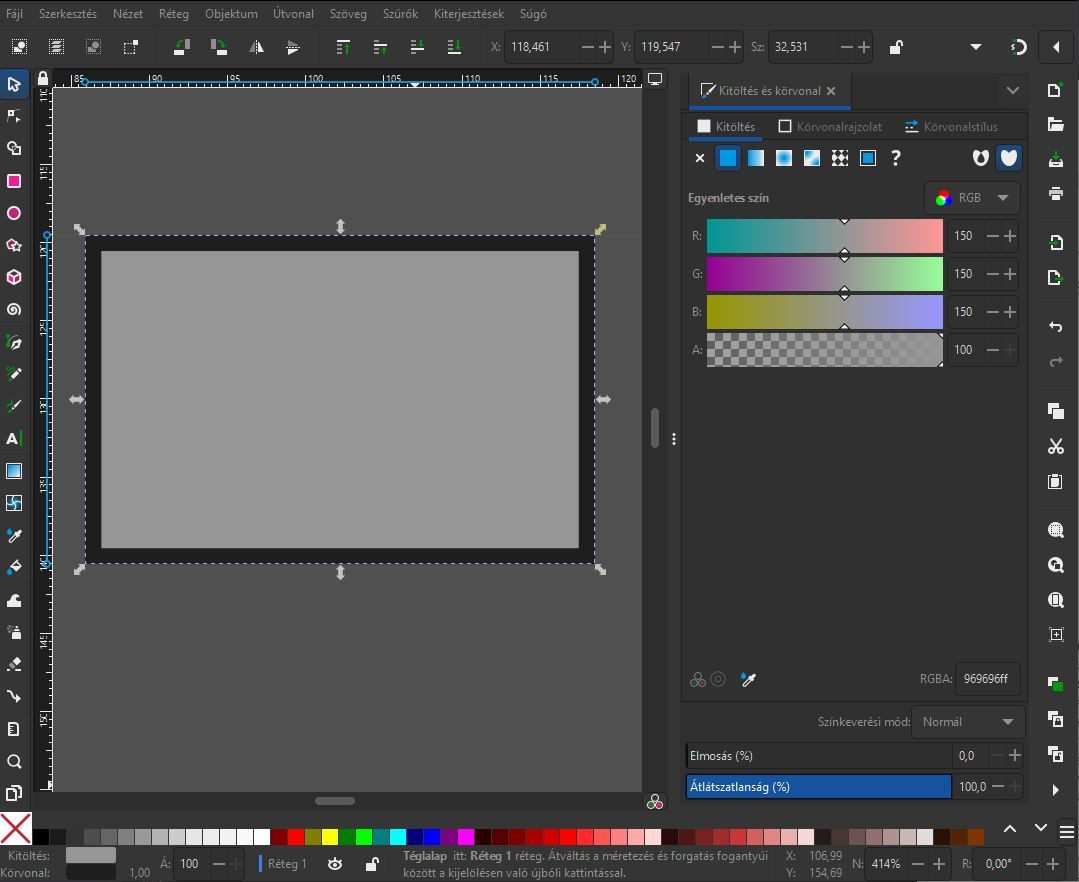
\includegraphics[width=0.8\textwidth,height=0.6\textwidth,keepaspectratio]{images/concept/inkscape.JPG}
\caption{Az Inkscape kezelőfelülete~\cite{inkscape}}
\label{fig:inkscape}
\end{figure}

Az Inkscape (\ref{fig:inkscape}. ábra) ingyenes, nyílt forráskódú asztali vektorgrafikus program Windows, macOS és Linux rendszerre~\cite{inkscape}, alapformátuma az SVG. A felülete sűrű. Bal oldalon az eszköztár, felül a menüsor és az aktuális eszköz beállításait tartalmazó sáv látható, jobb oldalon dokkolható párbeszédablakok, alul a színpaletta és az állapotsor.

Az alapalakzatok mellett csillagot, spirált és szabadkézi vonalakat is rajzol, és minden tulajdonság számszerűen is megadható a párbeszédablakokban. Az XML-szerkesztő fa szerkezetben mutatja a dokumentumot, és bármely attribútum közvetlenül módosítható benne. Az útvonalszerkesztés a program erőssége, a csomóponteszköz minden csomópontot és fogantyút elérhetővé tesz, a csomópontok típusa sarok és sima között váltható. Az útvonalakon unió, különbség, metszet, kizárás és felosztás végezhető, emellett útvonal elvágására és összevonására is van parancs~\cite{inkscape-boolean}. Az Alakzatépítő eszköz egymást metsző alakzatokból kattintásokkal állít össze új alakzatot~\cite{inkscape-1-3}.

A szöveg a vásznon és egy külön szövegablakban is szerkeszthető, útvonalra illeszthető, a betű- és sorköz és az alávágás is állítható. A színek RGB, HSL, HSV, CMYK és OKHSL színmódban adhatók meg~\cite{inkscape-1-3}. A kitöltés lehet lineáris, sugárirányú vagy hálós színátmenet és minta is. A rétegek és objektumok egy fában jelennek meg, ahol zárolhatók és elrejthetők, az illesztés pedig a rácshoz, a segédvonalakhoz és a más objektumok jellemző pontjaihoz egyaránt beállítható. Az előzmények külön panelen láthatók, az automatikus mentés pedig a beállításokban szabályozható.

\subsection{SVG-Edit}

\begin{figure}[H]
\centering
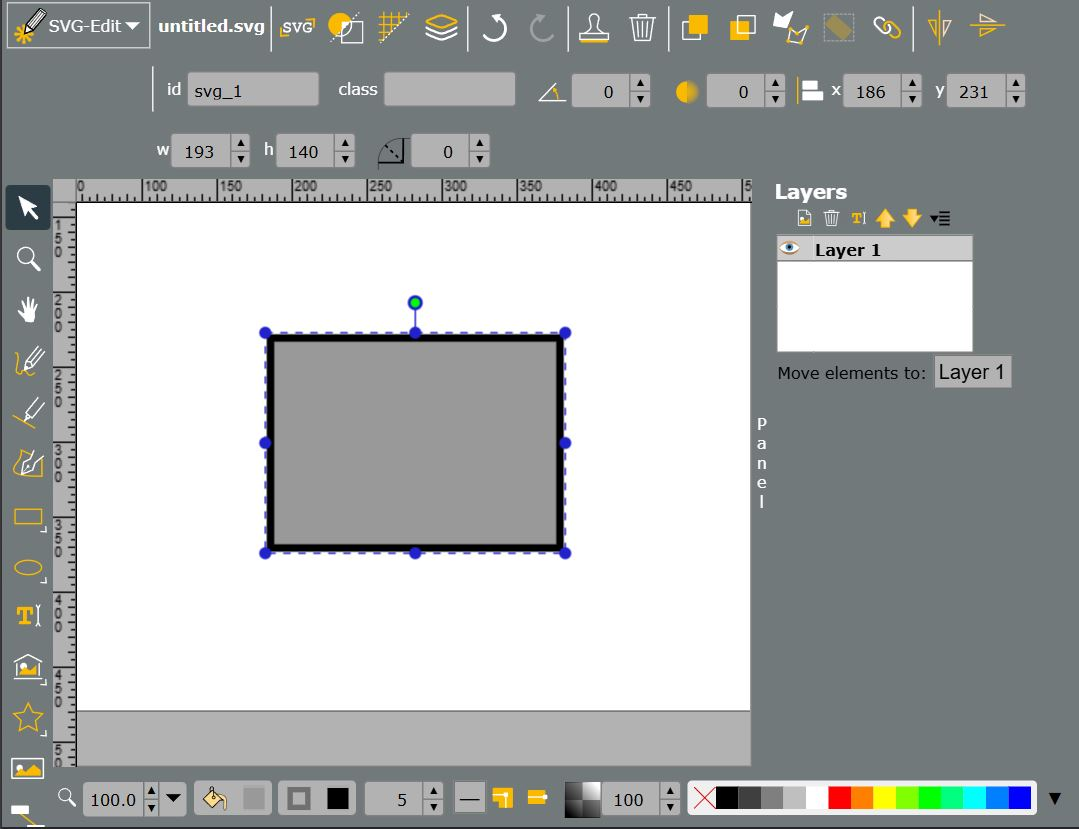
\includegraphics[width=0.8\textwidth,height=0.6\textwidth,keepaspectratio]{images/concept/svg-edit.JPG}
\caption{Az SVG-Edit kezelőfelülete~\cite{svg-edit}}
\label{fig:svg-edit}
\end{figure}

Az SVG-Edit (\ref{fig:svg-edit}. ábra) nyílt forráskódú, MIT licencű webes szerkesztő, amely regisztráció nélkül, közvetlenül a böngészőben fut~\cite{svg-edit,svgedit-github}. A felület tetején a kijelölt elem beállításai, bal oldalon az eszköztár, alul a kitöltés és a körvonal vezérlői, jobb oldalon a rétegpanel található.

Az alapalakzatok mellett egy beépített alakzatkönyvtárat is kínál. A forráskód-szerkesztő ablakban a teljes SVG-kód módosítható, a változtatások a módosítások alkalmazása után jelennek meg a vásznon. Az útvonalak csomópontjai mozgathatók, törölhetők és klónozhatók, a szakaszok típusa egyenes és görbe között váltható, a két kontrollpont pedig összekapcsolható. Logikai műveleteket nem kínál~\cite{svgedit-github}.

A szöveg a vásznon szerkeszthető, a betűstílus, a díszítővonalak, a betű- és szóköz, valamint az igazítás állítható. A beviteli mező csak egysoros szöveget fogad, és nyolc betűcsalád közül lehet választani~\cite{svgedit-github}. A színválasztó HEX, RGB és HSV értékeket fogad átlátszósággal együtt, a kitöltés egyszínű, lineáris vagy sugárirányú színátmenet lehet. Az illesztés a rácshoz kapcsolható be, az igazító parancsok több elemre is működnek. A visszavonás és a megismétlés elérhető, egy bővítmény pedig a lap bezárásakor a böngésző helyi tárolójába menti a rajzot, ha a felhasználó ezt engedélyezi.

\subsection{Boxy SVG}

\begin{figure}[H]
\centering
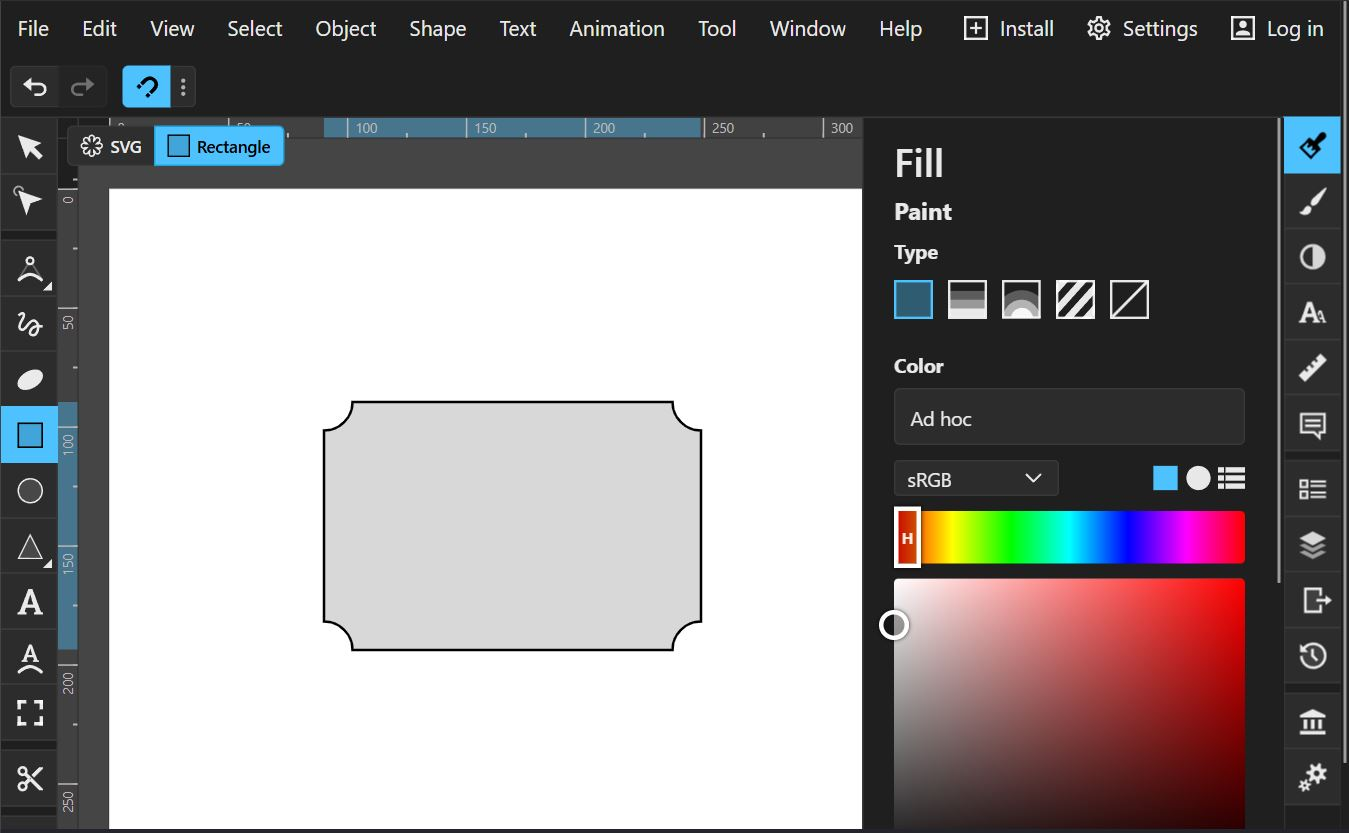
\includegraphics[width=0.8\textwidth,height=0.6\textwidth,keepaspectratio]{images/concept/boxy-svg.JPG}
\caption{A Boxy SVG kezelőfelülete~\cite{boxy-svg}}
\label{fig:boxy-svg}
\end{figure}

A Boxy SVG (\ref{fig:boxy-svg}. ábra) zárt forráskódú, freemium~\cite{freemium} vektorgrafikus szerkesztő, vagyis az alapváltozata ingyenes, a további szolgáltatásai pedig fizetősek. Webalkalmazásként és asztali alkalmazásként is elérhető. A webalkalmazás alapvető szerkesztő- és exportálási funkciói regisztráció és fizetés nélkül is használhatók, az asztali alkalmazások egy része és a haladó funkciók, például az automatikus felhőszinkronizálás és a teljes verziótörténet, viszont előfizetéshez kötöttek~\cite{boxy-svg}. A felület tetején menüsor van, alatta egy sáv a csoportosításhoz, igazításhoz, forgatáshoz és a logikai műveletekhez. A vásznat vonalzók veszik körül, a tulajdonságok a jobb oldali sávból nyíló panelekben állíthatók.

Az alapelemek mellett gyakori alakzatok, például háromszög és csillag is rajzolhatók. Az útvonalakhoz szabadkézi, másod- és harmadfokú görberajzoló eszköz tartozik, a csomópontok fogantyúkkal szerkeszthetők. Az alakzatokon unió, különbség, metszet, kizárás és felosztás végezhető. Az Elemek panel a dokumentum szerkezetét és SVG-kódját mutatja, a kód közvetlenül szerkeszthető, és az animációk kulcskockái is szerkeszthetők~\cite{boxy-svg}.

A szöveg a vásznon szerkeszthető és útvonalra illeszthető, a betűtípusok a Google Fonts gyűjteményéből, a gépre telepített vagy fájlból betöltött betűtípusok közül választhatók. A színek tizenkét színtérben adhatók meg, a szabványos és a széles színtartományú RGB-terektől az emberi színérzékelést követő CIE- és OK-modellekig, egy szöveges mezőben pedig HEX kóddal is. A kitöltés lineáris és sugárirányú színátmenet vagy minta is lehet, a gyakran használt színek, színátmenetek és minták a \lstinline[language=XML]|<defs>| elemben tárolhatók. Az elrendezést segédvonalak, intelligens segédvonalak és rács segítik, a visszavonható lépések pedig előzménypanelen láthatók.

\subsection{Figma}

\begin{figure}[H]
\centering
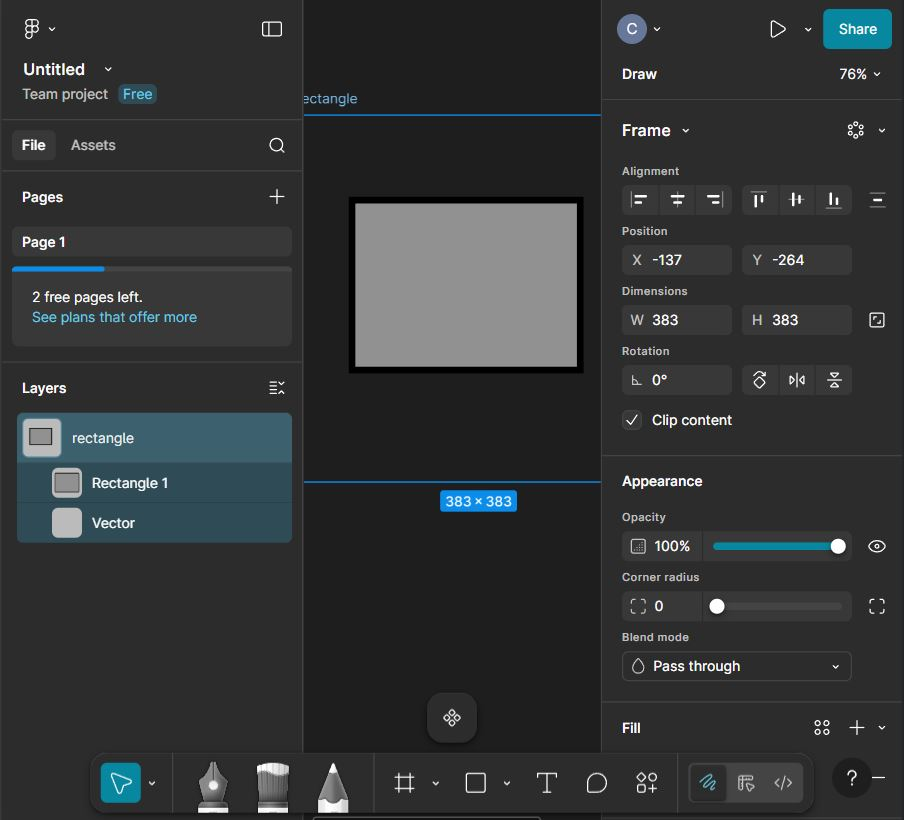
\includegraphics[width=0.8\textwidth,height=0.6\textwidth,keepaspectratio]{images/concept/figma.JPG}
\caption{A Figma kezelőfelülete~\cite{figma}}
\label{fig:figma}
\end{figure}

A Figma (\ref{fig:figma}. ábra) böngészőben és asztali alkalmazásként is futó felülettervező eszköz, amely szintén freemium konstrukcióban, ingyenes alapcsomaggal és előfizetéses csomagokkal érhető el~\cite{figma}. A rajzokat saját formátumban tárolja, az SVG számára csak importálási és exportálási formátum. A felület közepén a vászon van, bal oldalon a rétegek, jobb oldalon a tulajdonságok, az eszköztár pedig a vászon alján található~\cite{figma-ui3}.

Egy menüből téglalap, vonal, nyíl, ellipszis, sokszög, csillag és kép helyezhető el~\cite{figma-toolbar}. Az útvonalak helyett a Figma vektorhálózatokkal dolgozik, amelyekben egy csomópontból kettőnél több szakasz is indulhat~\cite{figma-vector-networks}. Az unió, a különbség, a metszet és a kizárás roncsolásmentes, az eredmény egy logikai csoport, amelynek tagjai később is módosíthatók~\cite{figma-boolean}. SVG-kódot a szerkesztő nem mutat, és az közvetlenül nem is módosítható.

A Google Fonts betűtípusai alapértelmezés szerint elérhetők, a gépre telepített betűtípusokhoz egy segédprogramra van szükség~\cite{figma-fonts}. A színválasztó HEX, HSB, HSL, CSS és RGB formátumot ismer~\cite{figma-color}, a kitöltés lehet egyszínű, színátmenet, minta, kép vagy videó. A rétegek fa szerkezetben jelennek meg. A munka folyamatosan a felhőbe mentődik, a verziótörténet az ingyenes csomagban 30 napra visszamenőleg érhető el~\cite{figma-history}.

\subsection{Mediamodifier}

\begin{figure}[H]
\centering
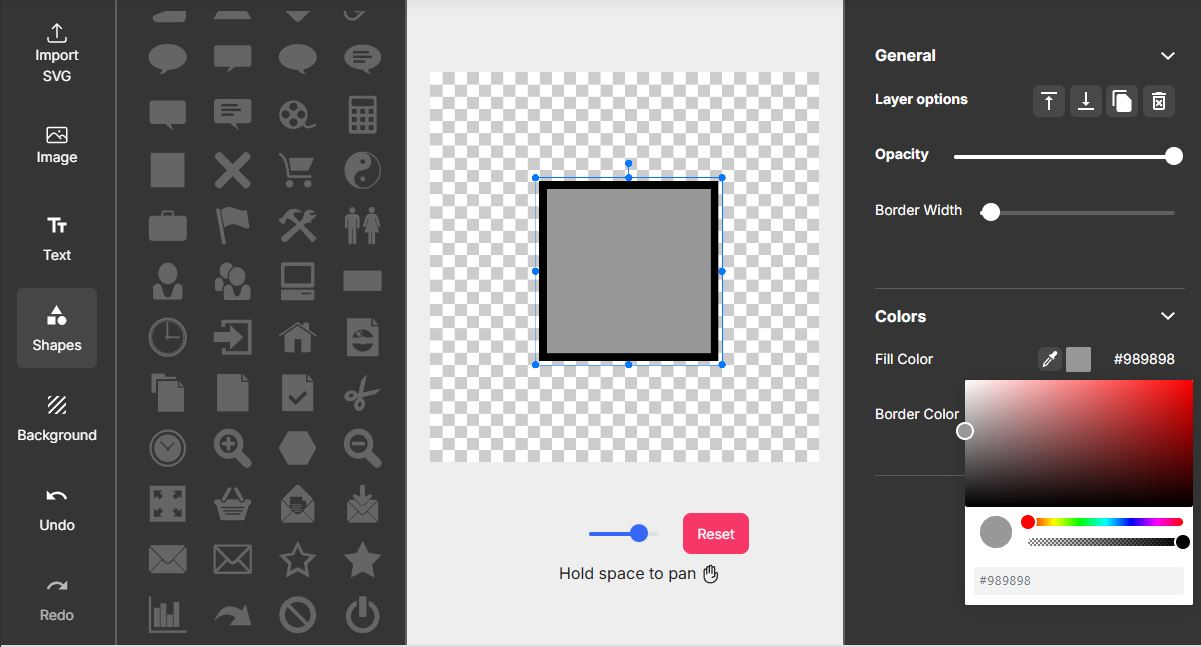
\includegraphics[width=0.8\textwidth,height=0.6\textwidth,keepaspectratio]{images/concept/mediamodifier.JPG}
\caption{A Mediamodifier kezelőfelülete~\cite{mediamodifier}}
\label{fig:mediamodifier}
\end{figure}

A Mediamodifier (\ref{fig:mediamodifier}. ábra) online grafikai és termékbemutató-készítő szolgáltatás, amely egy SVG-szerkesztőt is kínál~\cite{mediamodifier}. A szerkesztés ingyenes, a kész munka letöltéséhez azonban előfizetés szükséges. Egyszerű felületén bal oldalon az eszközsáv, jobb oldalon a tulajdonságok, középen a vászon található.

A szerkesztő kész elemek összeállítására épül. SVG-fájlok húzással helyezhetők a vászonra és kombinálhatók, az elemek csoportosíthatók, csoportbontással egyenként módosíthatók, és előrébb vagy hátrébb hozhatók~\cite{mediamodifier}. A kitöltés és a körvonal színe, valamint a körvonal vastagsága állítható. A kipróbálás során az alapalakzatok kész matricaként viselkedtek, a görbék rajzolására és az útvonalak szerkesztésére nem találtam lehetőséget, és a beimportált fájlok közül csak az egyszerű alakzatokból állók jelentek meg hibátlanul. A szöveg a vásznon szerkeszthető, de csak a betűtípus és a szín választható meg. Az SVG-kód nem érhető el.

\subsection{Összehasonlítás}
\label{sub:editor_comparison}

Az összehasonlítás szempontjait úgy választottam meg, hogy egy SVG-szerkesztő mindennapi használatát fedjék le. A felület elrendezésénél azt vizsgáltam, hogy az eszközök a megszokott helyen, logikusan csoportosítva érhetők-e el, és hogy a tulajdonságok számszerűen is megadhatók-e. Fejlesztői szempontból fontos, hogy a szerkesztő megmutatja-e az előállított SVG-kódot, és módosítható-e közvetlenül.

A rajzolás és szerkesztés szempontjai az útvonalakra összpontosítanak: hozzáadhatók és törölhetők-e a csomópontok, kényelmesen mozgathatók-e a fogantyúk, és elérhetők-e a logikai műveletek, vagyis az unió, a különbség, a metszet, a kizárás és a felosztás. Ide tartozik az illesztés a rácshoz és más objektumokhoz is. A szövegnél a többsoros bevitel, a vásznon történő szerkesztés és a betűtípusok forrása számít, a színeknél a színmegadás módjai, az átlátszóság, a színátmenetek és a minták.

A dokumentum kezelésénél a rétegek és csoportok megjelenítését, az előzményeket és a mentést vizsgáltam. A kijelölés, a nagyítás és a vágólap alapműveletei minden vizsgált szerkesztőben működtek, ezért ezeket a táblázat külön nem tünteti fel. \Aref{tab:svg-editors-comparison}. táblázat az eredményt foglalja össze.

\begin{table}[!htbp]
\caption{A vizsgált SVG-szerkesztők összehasonlítása}
\label{tab:svg-editors-comparison}
\centering
\scriptsize
\renewcommand{\arraystretch}{1.25}
\begin{adjustbox}{max width=\textwidth}
\begin{tabular}{|>{\raggedright\arraybackslash}p{2.0cm}|>{\raggedright\arraybackslash}p{2.5cm}|>{\raggedright\arraybackslash}p{2.5cm}|>{\raggedright\arraybackslash}p{2.5cm}|>{\raggedright\arraybackslash}p{2.5cm}|>{\raggedright\arraybackslash}p{2.3cm}|}
\hline
 & \textbf{Inkscape} & \textbf{SVG-Edit} & \textbf{Boxy SVG} & \textbf{Figma} & \textbf{Mediamodifier} \\ \hline
\textbf{Platform, licenc} & asztali, nyílt forráskódú & webes, nyílt forráskódú & webes és asztali, freemium & webes és asztali, freemium & webes, letöltés előfizetéssel \\ \hline
\textbf{Elrendezés} & klasszikus, dokkolható panelekkel & klasszikus, alsó stílussávval & klasszikus, beúszó panelekkel & vászon középen, eszköztár alul & egyszerű, két oldalsávval \\ \hline
\textbf{SVG-kód} & XML-szerkesztő & forrásablak, alkalmazás után frissül & Elemek panel, szerkeszthető & nincs & nincs \\ \hline
\textbf{Szöveg} & többsoros, útvonalra illeszthető & egysoros, 8 betűcsalád & útvonalra illeszthető, Google Fonts & Google Fonts, helyi betűtípusok & betűtípus és szín \\ \hline
\textbf{Színek} & RGB, HSL, HSV, CMYK, OKHSL & HEX, RGB, HSV, átlátszóság & 12 színtér (RGB, CIE, OK), HEX & HEX, HSB, HSL, CSS, RGB & színválasztó \\ \hline
\textbf{Színátmenet, minta} & lineáris, sugárirányú, hálós; minta & lineáris, sugárirányú & lineáris, sugárirányú; minta & színátmenetek, minta, kép & egyszínű \\ \hline
\textbf{Útvonalak} & teljes csomópont-szerkesztés & csomópontok, szakasztípus & csomópontok, fogantyúk & vektorhálózatok & nincs \\ \hline
\textbf{Logikai műveletek} & unió, különbség, metszet, kizárás, felosztás & nincs & unió, különbség, metszet, kizárás, felosztás & unió, különbség, metszet, kizárás & nincs \\ \hline
\textbf{Illesztés} & rács, segédvonalak, objektumok & rács & rács, segédvonalak & igazítási segédvonalak & alapszintű \\ \hline
\textbf{Rétegek} & objektumfa, zárolás & rétegpanel & elemfa & rétegfa & előre-hátra mozgatás \\ \hline
\textbf{Előzmények, mentés} & előzménypanel, automatikus mentés & visszavonás, mentés a lap bezárásakor & előzménypanel, felhőtárhely & verziótörténet, folyamatos felhőmentés & letöltés előfizetéssel \\ \hline
\end{tabular}
\end{adjustbox}
\end{table}

\subsection{Következtetések és célkitűzések}
\label{sub:editor_conclusions}

A vizsgált szerkesztők közül az Inkscape kínálja a legteljesebb SVG-szerkesztést, de asztali program, amelyet telepíteni kell. A Boxy SVG hasonlóan sokoldalú, böngészőben is fut, haladó funkciói azonban előfizetéshez kötöttek, és a forráskódja zárt. A Figma kiváló vektoros eszközei saját adatmodellre épülnek, az SVG csak be- és kimeneti formátum. A Mediamodifier kész elemek összeállítására készült, görbéket nem lehet vele rajzolni. Az SVG-Edit ingyenes és nyílt forráskódú, kódnézetet is kínál, de csak egysoros szöveget kezel, és logikai műveletek nincsenek benne.

% A vizsgált alkalmazások többsége a klasszikus elrendezést követi, amely más grafikai programokból is ismerős.

Ezek alapján a saját szerkesztővel szemben a következő célokat tűztem ki:

\begin{enumerate}
\item A szerkesztő szerver, telepítés és regisztráció nélkül, ingyenesen fusson a böngészőben, klasszikus elrendezéssel.
\item Kínáljon a vizsgált szerkesztőkhöz mérhető rajzoló és szerkesztő eszközöket, köztük teljes értékű útvonalszerkesztést és logikai műveleteket, amelyek eredménye görbékből álló, tovább szerkeszthető alakzat marad.
\item Kezeljen többsoros szöveget, és alakítsa útvonallá úgy, hogy az eredmény megegyezzen a képernyőn látottal.
\item Importáljon SVG-fájlokat, és jelezze, milyen szerkezeteket nem tud kezelni.
\item Exportáljon szabványos SVG-fájlt és raszteres képet.
\item Legyen telefonon és táblagépen is kezelhető.
\end{enumerate}

\Aref{ch:requirements}. fejezet ezeket a célokat bontja részletes követelményekre, \aref{ch:evaluation}. fejezet pedig azt értékeli, mennyiben teljesültek.

\chapter{Tervezés}
\label{ch:requirements}

A fejezet a saját szerkesztővel szemben támasztott követelményekkel kezdődik, amelyek \aref{sub:editor_comparison}. alszakasz szempontjait követik. Ezután a felület terve, a felhasznált technológiák, az alkalmazás rétegei, az adatmodell, az előzmények kezelése, az eszközök közös felülete és a tárolás következik.

\section{Követelmények}
\label{sec:requirements}

\Aref{sub:editor_conclusions}. alszakasz célkitűzései még csak az irányt jelölik ki. Ez a szakasz ezeket ellenőrizhető funkcionális és nem funkcionális követelményekre bontja.

\subsection{Funkcionális követelmények}

\Aref{tab:requirements}. táblázat a funkcionális követelményeket sorolja fel. A területek nagyrészt megegyeznek \aref{tab:svg-editors-comparison}. táblázat soraival, így szempontonként összevethető, melyik megoldást követi a saját szerkesztő. Az utolsó oszlop azt mutatja, melyik célkitűzéshez tartozik az adott követelmény. Az azonosítókra a tesztelés és az értékelés is hivatkozik.

\begin{table}[!htbp]
\caption{Funkcionális követelmények}
\label{tab:requirements}
\centering
\footnotesize
\renewcommand{\arraystretch}{1.2}
\begin{tabular}{|l|>{\raggedright\arraybackslash}p{0.19\textwidth}|>{\raggedright\arraybackslash}p{0.56\textwidth}|c|}
\hline
\textbf{Az.} & \textbf{Terület} & \textbf{Követelmény} & \textbf{Cél} \\ \hline
F1 & Elrendezés & Felül menüsor és a helyzethez igazodó parancssáv, bal oldalon eszköztár, középen vonalzós vászon, jobb oldalon tulajdonságpanel. Keskeny kijelzőn a panel alulról nyílik. & 1, 6 \\ \hline
F2 & Rajzolás & Téglalap, ellipszis, vonal, sokszög és töröttvonal, Bézier-görbéket rajzoló toll, körív, szabadkézi rajz és szöveg, csoportosítva az eszköztáron. & 2 \\ \hline
F3 & Tulajdonságok & Minden alakzat módosítható a vásznon fogantyúkkal és a panelen számszerűen, elforgatva is. Több kijelölt alakzat együtt mozgatható és méretezhető. & 2 \\ \hline
F4 & SVG-kód & Kódszerkesztő nincs, a kimenet szabványos, olvasható SVG. & 5 \\ \hline
F5 & Szöveg & Többsoros szöveg a vásznon szerkesztve. Betűtípus, méret, vastagság, dőlt stílus, díszítővonalak, betű- és szóköz, sorköz és igazítás. Útvonallá alakítás a képernyőn látottal egyező eredménnyel. & 3 \\ \hline
F6 & Színek & HEX, RGB és HSL színmegadás átlátszósággal, lineáris és sugárirányú színátmenet, szaggatás, vonalvég, sarok és kitöltési szabály. & 2 \\ \hline
F7 & Útvonalak & Csomópontok hozzáadása, törlése, mozgatása és többes kijelölése, váltás sarok és sima csomópont között, a fogantyúk mozgatása. Unió, különbség, metszet, kizárás és felosztás, alakzatok vágása, körvonal útvonallá alakítása. & 2 \\ \hline
F8 & Illesztés, igazítás & Illesztés rácshoz, más alakzatok széleihez és középvonalaihoz, a vonalzókból húzott segédvonalakhoz. Igazító parancsok több alakzatra. & 2 \\ \hline
F9 & Objektumok & Csoportosítás és belépés a csoportba, az alakzatok fája, a sorrend módosítása húzással, elrejtés és zárolás. & 2 \\ \hline
F10 & Kijelölés & Kattintás, bővítés Shift billentyűvel, területkijelölés. Érintőképernyőn a Shift helyett bekapcsolható gomb. & 2, 6 \\ \hline
F11 & Vágólap & A szokásos billentyűkombinációk, másolás más programokba és más programokból, valamint a szerkesztő böngészőlapjai között. & 2 \\ \hline
F12 & Nagyítás & Görgővel a kurzor körül, gombokkal, a lapra illesztve, érintőképernyőn két ujjal. & 2, 6 \\ \hline
F13 & Visszavonás & Minden módosítás visszavonható és megismételhető, a lépések névvel jelennek meg. Egy folyamatos állítás egyetlen lépés. & 2 \\ \hline
F14 & Mentés & Folyamatos automatikus mentés a böngészőbe és visszatöltés újranyitáskor, mentés projektfájlba. & 1 \\ \hline
F15 & Import, export & SVG-fájlok és raszteres képek importálása, a nem támogatott szerkezetekről figyelmeztetés. Exportálás SVG, PNG, JPG és WebP formátumba. & 4, 5 \\ \hline
\end{tabular}
\end{table}

Az F4 követelmény külön indoklást kíván, mert a szerkesztő nem tartalmaz kódszerkesztőt, holott \aref{sec:svg_editors}. szakaszban vizsgált programok közül három is kínál ilyet. A szerkesztő saját adatmodellel dolgozik, amelyet \aref{sec:data_model}. szakasz ír le, egy élő kódszerkesztőnek tehát minden begépelt változtatást ellenőriznie és erre a modellre kellene alakítania. Ez lényegében az importáló folyamatos futtatását jelentené, ezért a kódnézetet a továbbfejlesztési lehetőségek közé soroltam.

\subsection{Nem funkcionális követelmények}

Az első célkitűzésből következik, hogy az alkalmazás kizárólag a böngészőben futhat. A fájlok a felhasználó gépén maradnak, hálózatra csak a Google Fonts betűtípusainak letöltéséhez van szükség. A felületnek asztali gépen, táblagépen és telefonon is használhatónak kell lennie. Keskeny kijelzőn a tulajdonságpanel nem takarhatja el a rajzot, és az érintéssel használt fogantyúknak elég nagynak kell lenniük.

A felület tervezésekor Nielsen tíz használhatósági heurisztikája közül négyre figyeltem különösen~\cite{nielsen-heuristics}. A rendszer állapotának láthatóságát az elnevezett előzménylépések szolgálják, a felhasználó szabadságát pedig az, hogy bármely korábbi állapotba visszaléphet. A megszokott konvenciókhoz igazodnak a más grafikus programokéval egyező billentyűkombinációk. A felismerés előnyben részesítése az emlékezéssel szemben a parancssávban valósul meg, amely mindig az adott helyzetben elérhető műveleteket mutatja.

Egy sérült vagy szándékosan rosszul összeállított fájl nem teheti használhatatlanná a szerkesztőt, ezért a betöltött projektfájlokat mezőnként ellenőrizni kell, és a hibás részeket el kell dobni. Végül a geometriai számításokat, az előzményeket és a fájlkezelést automatikus teszteknek kell ellenőrizniük.

\section{A felhasználói felület terve}
\label{sec:ui_design}

A felület tervezésekor az elrendezésből indultam ki, amelyet \aref{fig:layout}. ábra mutat. A szerkesztő angol nyelvű, ezért az ábrán és a későbbi képernyőképeken angol feliratok láthatók, a szöveg pedig ezek magyar megfelelőit használja.

\begin{figure}[!htbp]
\centering
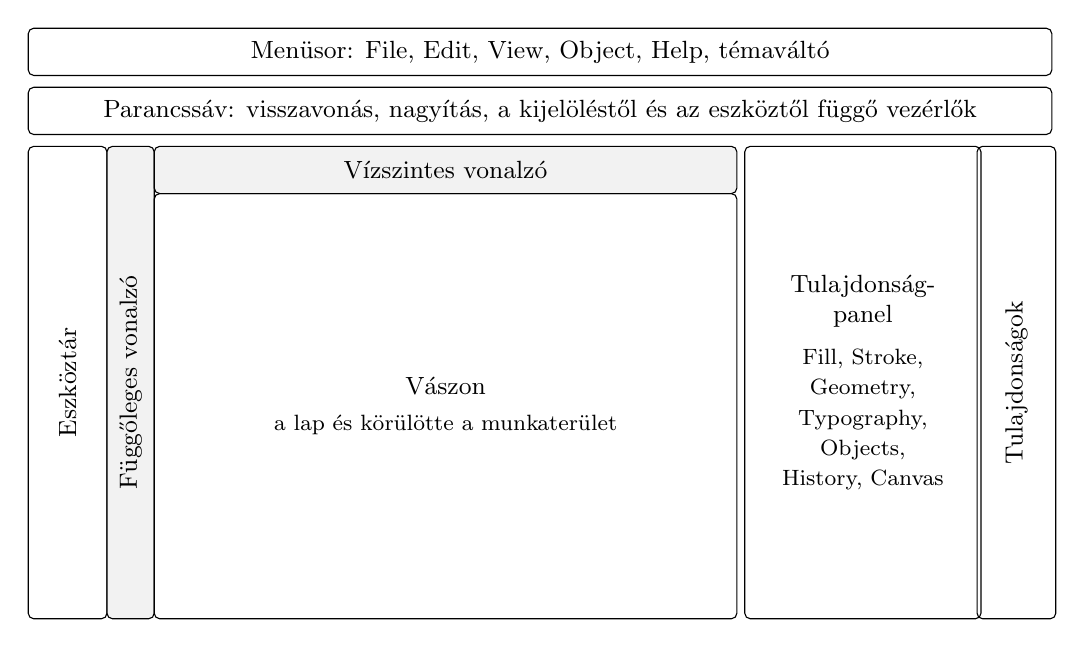
\begin{tikzpicture}[
  box/.style={draw, rounded corners=2pt, align=center, font=\small, inner sep=3pt},
  x=1cm, y=1cm]
  \node[box, minimum width=13cm, minimum height=0.6cm] (menu) at (6.5,7.3) {Menüsor: File, Edit, View, Object, Help, témaváltó};
  \node[box, minimum width=13cm, minimum height=0.6cm] (cmd) at (6.5,6.55) {Parancssáv: visszavonás, nagyítás, a kijelöléstől és az eszköztől függő vezérlők};
  \node[box, minimum width=1cm, minimum height=6cm] (tools) at (0.5,3.1) {\rotatebox{90}{Eszköztár}};
  \node[box, minimum width=0.6cm, minimum height=6cm, fill=black!5] (rulerv) at (1.3,3.1) {\rotatebox{90}{Függőleges vonalzó}};
  \node[box, minimum width=7.4cm, minimum height=0.6cm, fill=black!5] (rulerh) at (5.3,5.8) {Vízszintes vonalzó};
  \node[box, minimum width=7.4cm, minimum height=5.4cm] (canvas) at (5.3,2.8) {Vászon\\[2pt]\footnotesize a lap és körülötte a munkaterület};
  \node[box, minimum width=3cm, minimum height=6cm] (panel) at (10.6,3.1) {Tulajdonság-\\panel\\[4pt]\footnotesize Fill, Stroke,\\\footnotesize Geometry,\\\footnotesize Typography,\\\footnotesize Objects,\\\footnotesize History, Canvas};
  \node[box, minimum width=1cm, minimum height=6cm] (tabs) at (12.55,3.1) {\rotatebox{90}{Tulajdonságok}};
\end{tikzpicture}
\caption{A felület elrendezése asztali kijelzőn}
\label{fig:layout}
\end{figure}

A menüsor a ritkábban használt, de mindig elérhető parancsokat gyűjti össze: a fájlkezelést, a szerkesztési műveleteket, a nézet beállításait, az objektumokra vonatkozó műveleteket és a súgót. A parancssáv bal szélén mindig ott van a visszavonás, a megismétlés és a nagyítás, a többi vezérlője az aktuális eszköztől és a kijelöléstől függ. Egy kijelölt alakzatnál a forgatás, az átlátszóság és a tükrözés jelenik meg, több alakzatnál az igazítás és a logikai műveletek, a tollnál pedig egy rövid útmutató a használatához.

A bal oldali eszköztár tizenhárom eszköze hat csoportot alkot. Az első a kijelölés és a csomópontok szerkesztése, a második a vonalak és görbék rajzolása, a harmadik a zárt alakzatoké. Ezt követi a szöveg, majd a meglévő alakzatokon dolgozó foltecset és olló, végül a nézet mozgatása. Minden eszköznek saját billentyűje van, ezeket a súgó is felsorolja.

A jobb oldali tulajdonságsáv hét panelt nyit meg. A kitöltés és a körvonal panel a színeket és a vonal stílusát állítja. A geometria panelen a pozíció, a méret, a forgatás és a forgatási középpont adható meg, a tipográfia panelen a szöveg beállításai. Az objektumok panel a dokumentum fáját mutatja, az előzmények panel a visszavonható lépéseket, a vászon panel a lap méretét, hátterét, a rácsot és az illesztést. A panel szélessége húzással állítható, a nyitott panel fülére újra kattintva pedig a panel bezárul, és a vászon a teljes szélességet megkapja.

Keskeny kijelzőn a panel már nem férne el a rajz mellett. Ilyenkor a vászon alatt, alulról nyíló lapként jelenik meg, amelynek magassága a felső szélénél húzva állítható. Az eszköztár és a tulajdonságsáv a helyén marad, így nyitott panel mellett is elérhetők.

A műveletek többféle úton érhetők el, de egyik sem csak rejtett úton. A gyakoriak a parancssávban vannak, a helyzethez kötöttek a jobb gombbal vagy hosszú érintéssel nyíló helyi menüben, és a menüsor mindegyiket tartalmazza. A helyi menü csak az adott helyzetben végrehajtható műveleteket sorolja fel, mert a letiltott menüpontok nehezebben áttekinthetővé tennék.

\section{Technológiai választások}
\label{sec:technologies}

Az alkalmazás teljes egészében kliensoldali webalkalmazás, a technológiák kiválasztásakor ezért a böngészőben futó, szerver nélkül is használható megoldásokat kerestem. Ez a szakasz a keretrendszert, a fejlesztői eszközöket és a külső könyvtárakat mutatja be, \aref{tab:versions}. táblázat pedig a pontos verziókat is rögzíti.

\subsection{Svelte és TypeScript}

A Svelte komponensei egyetlen fájlban írják le a szerkezetet, a stílust és a viselkedést, a fordító pedig ezekből a DOM-ot közvetlenül módosító JavaScript kódot állít elő~\cite{svelte-overview}. Az alkalmazás állapotát Svelte \textit{store}-ok tárolják. A store olyan objektum, amelyre a komponensek feliratkozhatnak, és amely minden változásról értesíti őket~\cite{svelte-stores}. A származtatott store más store-ok értékéből számol, és csak akkor frissül, ha a forrása megváltozott. Egy szerkesztőben ugyanazt a dokumentumot a vászon, a panelek és az objektumlista egyszerre jeleníti meg, és ez a modell mindhármat automatikusan naprakészen tartja.

Általános komponenskönyvtárat, például a Bootstrapet, nem használtam. A szerkesztő vezérlői, a színválasztó, a csúszkák, a fogantyúk és az objektumlista, egyedi elemek, egy komponenskönyvtár pedig saját megjelenést és elrendezési szabályokat hozott volna, amelyek a sűrű szerkesztőfelülethez kevéssé illeszkednek.

A TypeScript használatát az adatmodell indokolja. Az alakzatok típusa egy közös típusmező szerint elágazó unió, angol nevén \textit{discriminated union}, és a típusellenőrzés segít észrevenni, ha egy függvény valamelyik alakzattípus kezelését kihagyja.

\subsection{Fejlesztői eszközök}

A projekt a Vite fejlesztői környezetet használja. Fejlesztés közben a Vite a forrásfájlokat natív ES modulokként szolgálja ki, ezért egy módosítás után elég az érintett modult újratölteni~\cite{vite}. Az éles változatot is a Vite csomagolja statikus fájlokká, amelyeket bármely webszerver kiszolgálhat.

A tesztek a Vitest keretrendszerrel futnak, amely a Vite beállításait használja, a komponensek teszteléséhez pedig a jsdom könyvtár ad böngészőszerű környezetet Node.js alatt~\cite{vitest,jsdom}. A böngészőben végzett ellenőrzések egy részét a Playwright eszközzel automatizáltam, amely programból vezérel egy Chromium böngészőt~\cite{playwright}.

\subsection{Geometriai és betűtípus-könyvtárak}

A geometriai algoritmusok többsége saját kód, három területen azonban külső könyvtárra támaszkodik a szerkesztő: a logikai műveleteknél és a vágásnál a paper.js, a körvonal útvonallá alakításánál és a foltecsetnél a Clipper, a szöveg útvonallá alakításánál pedig a fontkit könyvtárra. \Aref{tab:versions}. táblázat a fejlesztői eszközökkel együtt sorolja fel őket.

\begin{table}[!ht]
\caption{A felhasznált eszközök és könyvtárak}
\label{tab:versions}
\centering
\footnotesize
\begin{tabular}{|l|l|>{\raggedright\arraybackslash}p{0.55\textwidth}|}
\hline
\textbf{Név} & \textbf{Verzió} & \textbf{Szerep} \\ \hline
Svelte & 5.57.2 & felhasználói felület, állapotkezelés \\ \hline
TypeScript & 5.9.3 & programozási nyelv \\ \hline
Vite & 7.3.7 & fejlesztői szerver, éles változat csomagolása \\ \hline
Vitest & 3.2.7 & automatikus tesztek \\ \hline
jsdom & 26.1.0 & böngészőszerű környezet a tesztekhez \\ \hline
paper.js & 0.17.0 & logikai műveletek, alakzatok vágása \\ \hline
clipper-lib & 6.4.2 & körvonal útvonallá alakítása, foltecset \\ \hline
fontkit & 2.0.4 & szöveg útvonallá alakítása, OpenType-szövegszedés \\ \hline
woff2-encoder & 2.0.0 & WOFF2 betűtípusfájlok kibontása a fontkit számára \\ \hline
\end{tabular}
\end{table}

A sokszögek logikai műveleteire több klasszikus algoritmus ismert. Vatti söprővonalas algoritmusa tetszőleges, akár önmagukat metsző sokszögeket is kezel~\cite{vatti1992}, ennek továbbfejlesztése a Clipper könyvtár~\cite{clipper}. A Martínez-Rueda-Feito algoritmus $O((n+k)\log n)$ időben dolgozik, ahol $n$ a csúcsok, $k$ a metszéspontok száma~\cite{martinez2009}, ezt valósítja meg a polygon-clipping könyvtár~\cite{polygon-clipping}. A logikai műveletekhez a polygon-clipping és a clipper2-ts könyvtárat is megvizsgáltam. Mindkettő sokszögekkel dolgozik, a görbéket előbb rövid egyenes szakaszokra bontják. Két kör egyesítéséből így több száz sarokpontú alakzat lenne, amely kézzel már alig szerkeszthető. A paper.js a görbék metszéspontjait számolja ki, és az eredményt is görbékből építi fel~\cite{paperjs}. A körvonal útvonallá alakítása és a foltecset eredménye eleve sokszög, ezekhez a Clipper eltolási és egyesítési műveleteit használtam~\cite{clipper}.

\newpage

\section{Az alkalmazás rétegei}
\label{sec:architecture}

Az alkalmazás négy rétegből áll, ezeket és a köztük haladó adatfolyamot \aref{fig:architecture}. ábra mutatja.

\begin{figure}[!ht]
\centering
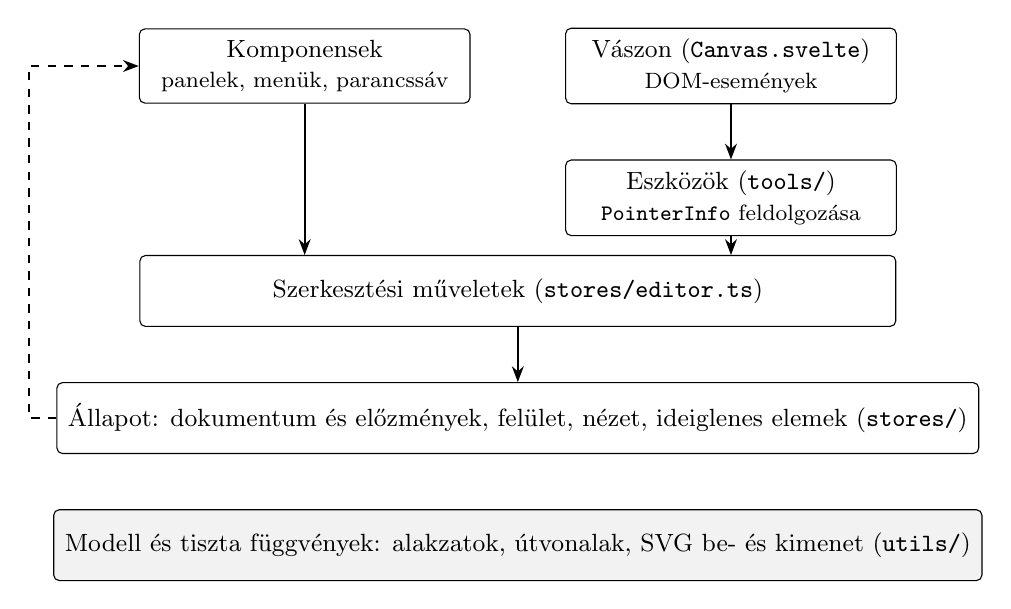
\begin{tikzpicture}[
  layer/.style={draw, rounded corners=2pt, align=center, font=\small, minimum height=0.9cm, inner sep=4pt},
  arr/.style={-{Stealth[length=2mm]}, thick},
  node distance=0.7cm and 0.8cm]
  \node[layer, minimum width=4.2cm] (ui) {Komponensek\\\footnotesize panelek, menük, parancssáv};
  \node[layer, minimum width=4.2cm, right=1.2cm of ui] (canvas) {Vászon (\texttt{Canvas.svelte})\\\footnotesize DOM-események};
  \node[layer, minimum width=4.2cm, below=of canvas] (tools) {Eszközök (\texttt{tools/})\\\footnotesize \texttt{PointerInfo} feldolgozása};
  \node[layer, minimum width=9.6cm, below=2.4cm of $(ui)!0.5!(canvas)$] (editor) {Szerkesztési műveletek (\texttt{stores/editor.ts})};
  \node[layer, minimum width=9.6cm, below=of editor] (stores) {Állapot: dokumentum és előzmények, felület, nézet, ideiglenes elemek (\texttt{stores/})};
  \node[layer, minimum width=9.6cm, below=of stores, fill=black!5] (utils) {Modell és tiszta függvények: alakzatok, útvonalak, SVG be- és kimenet (\texttt{utils/})};
  \draw[arr] (canvas) -- (tools);
  \draw[arr] (ui.south) -- (ui.south |- editor.north);
  \draw[arr] (tools.south) -- (tools.south |- editor.north);
  \draw[arr] (editor) -- (stores);
  \draw[arr, dashed] (stores.west) -- ++(-0.35,0) |- (ui.west);
\end{tikzpicture}
\caption{Az alkalmazás rétegei és az adatfolyam iránya; a szaggatott nyíl a store-ok értesítéseit jelöli}
\label{fig:architecture}
\end{figure}

A legalsó réteg az \texttt{utils} mappa. Itt van a dokumentum típusainak leírása és a mellékhatás nélküli, úgynevezett tiszta függvények: a határoló téglalapok számítása, az alakzatok mozgatása és méretezése, az útvonalak feldolgozása, az SVG importálása és előállítása. Ezek a függvények sosem módosítják a kapott alakzatot, hanem új alakzatot adnak vissza. Fölöttük a \texttt{stores} mappa store-jai tárolják a dokumentumot és az előzményeit, a felület állapotát a kijelöléssel és az aktuális eszközzel, a nézet nagyítását és eltolását, valamint az ideiglenes rajzelemeket, például a rajzolás közbeni előnézetet.

A dokumentumot csak az \texttt{editor} objektum műveletei módosítják. Ilyen az alakzat hozzáadása, a stílus módosítása, a csoportosítás, az igazítás, a logikai művelet és a beillesztés, és mindegyik egy elnevezett, visszavonható lépést hoz létre. A legfelső rétegben a rajzoló eszközök a vászontól kapják a mutató eseményeit, a komponensek pedig a felhasználó kattintásait. Mindkettő csak az \texttt{editor} műveleteit hívja, az eredményt pedig a store-okból olvassa vissza.

Ennek az egyirányú adatfolyamnak két haszna van. Egy művelet ugyanúgy viselkedik, akár a panelről, akár a menüből, akár a helyi menüből indítják. Az eszközök és a műveletek emellett böngésző nélkül is tesztelhetők, mert egy eszköz kipróbálásához elég mesterséges mutatóeseményeket átadni neki, majd megvizsgálni a dokumentumot.

\Aref{fig:move-sequence}. ábra ezt az adatfolyamot egy alakzat húzással történő mozgatásán mutatja be. A kijelölő eszköz a lenyomáskor előnézeti módba kapcsolja a dokumentumot, mozgatás közben csak az előnézetet frissíti, a felengedéskor pedig egyetlen elnevezett lépésként rögzíti a változást. A vászon a store-ra feliratkozva értesül minden módosításról, és ennek hatására rajzolja újra az alakzatokat.

\begin{figure}[!htbp]
\centering
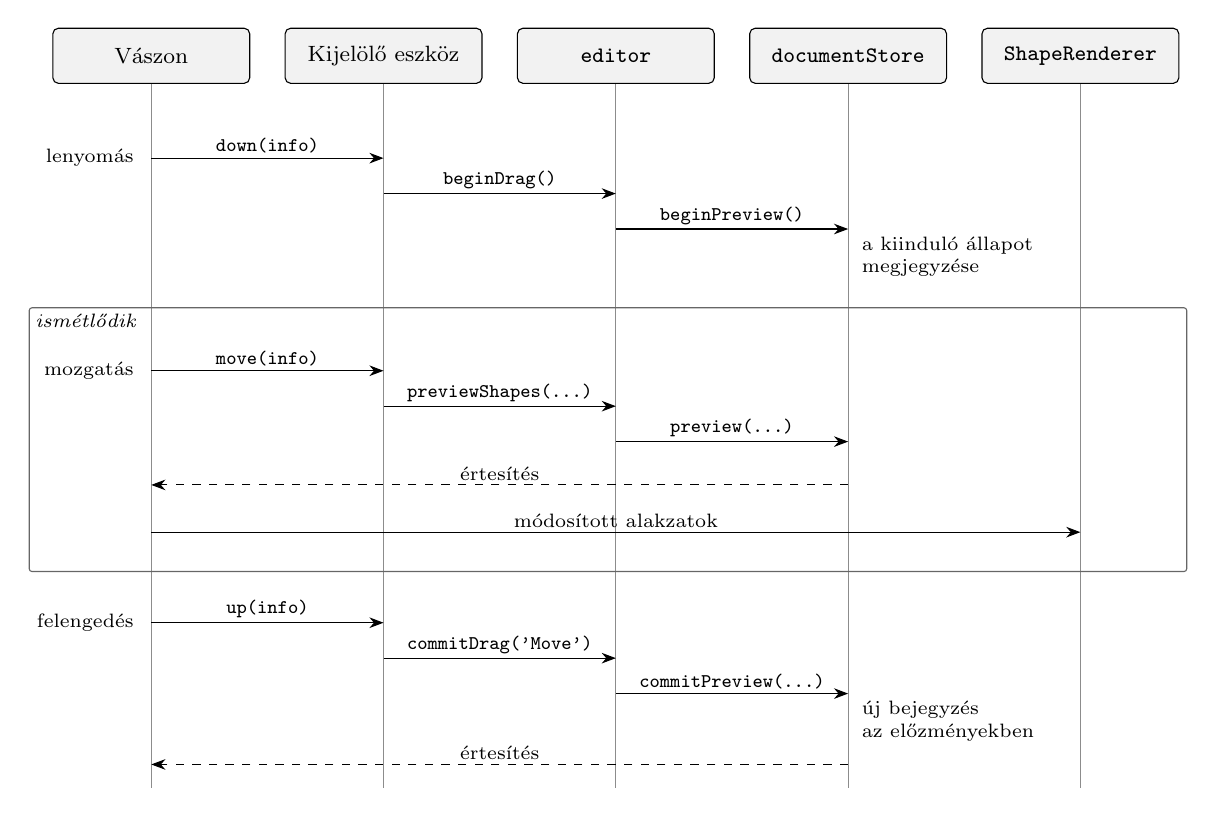
\begin{tikzpicture}[
  font=\footnotesize,
  head/.style={draw, rounded corners=2pt, fill=black!5, minimum width=2.5cm, minimum height=0.7cm, align=center},
  msg/.style={-{Stealth[length=1.8mm]}},
  ret/.style={-{Stealth[length=1.8mm]}, dashed},
  lbl/.style={above, inner sep=1.5pt, font=\scriptsize},
  note/.style={font=\scriptsize, align=left, anchor=west}]
  \foreach \x/\n/\t in {0/c/{Vászon}, 2.95/t/{Kijelölő eszköz}, 5.9/e/{\texttt{editor}}, 8.85/d/{\texttt{documentStore}}, 11.8/r/{\texttt{ShapeRenderer}}} {
    \node[head] (\n) at (\x,0) {\t};
    \draw[black!45] (\n.south) -- (\x,-9.3);
  }
  % lenyomás
  \node[font=\scriptsize, align=right, anchor=east] at (-0.1,-1.3) {lenyomás};
  \draw[msg] (0,-1.3) -- node[lbl] {\texttt{down(info)}} (2.95,-1.3);
  \draw[msg] (2.95,-1.75) -- node[lbl] {\texttt{beginDrag()}} (5.9,-1.75);
  \draw[msg] (5.9,-2.2) -- node[lbl] {\texttt{beginPreview()}} (8.85,-2.2);
  \node[note] at (8.9,-2.55) {a kiinduló állapot\\megjegyzése};
  % mozgatás ciklus
  \draw[black!60, rounded corners=1pt] (-1.55,-3.2) rectangle (13.15,-6.55);
  \node[anchor=north west, font=\scriptsize\itshape, inner sep=2pt] at (-1.55,-3.2) {ismétlődik};
  \node[font=\scriptsize, align=right, anchor=east] at (-0.1,-4.0) {mozgatás};
  \draw[msg] (0,-4.0) -- node[lbl] {\texttt{move(info)}} (2.95,-4.0);
  \draw[msg] (2.95,-4.45) -- node[lbl] {\texttt{previewShapes(\dots)}} (5.9,-4.45);
  \draw[msg] (5.9,-4.9) -- node[lbl] {\texttt{preview(\dots)}} (8.85,-4.9);
  \draw[ret] (8.85,-5.45) -- node[lbl] {értesítés} (0,-5.45);
  \draw[msg] (0,-6.05) -- node[lbl] {módosított alakzatok} (11.8,-6.05);
  % felengedés
  \node[font=\scriptsize, align=right, anchor=east] at (-0.1,-7.2) {felengedés};
  \draw[msg] (0,-7.2) -- node[lbl] {\texttt{up(info)}} (2.95,-7.2);
  \draw[msg] (2.95,-7.65) -- node[lbl] {\texttt{commitDrag('Move')}} (5.9,-7.65);
  \draw[msg] (5.9,-8.1) -- node[lbl] {\texttt{commitPreview(\dots)}} (8.85,-8.1);
  \node[note] at (8.9,-8.45) {új bejegyzés\\az előzményekben};
  \draw[ret] (8.85,-9.0) -- node[lbl] {értesítés} (0,-9.0);
\end{tikzpicture}
\caption{Egy alakzat mozgatásának lépései a rétegeken át; a szaggatott nyilak a store értesítéseit jelölik}
\label{fig:move-sequence}
\end{figure}

\section{Adatmodell}
\label{sec:data_model}

A dokumentum JSON formában tárolható adatszerkezet. Az alakzatok fáján kívül a lap méretét, a hátteret, egy opcionális háttérképet és a vonalzókból húzott segédvonalakat tartalmazza. Az alakzatok típusát a \texttt{type} mező adja meg, és ez dönti el, milyen geometriai adatok tartoznak hozzájuk. \Aref{tab:shape-types}. táblázat az alakzattípusokat és a kimenetben nekik megfelelő SVG-elemeket mutatja.

\begin{table}[!htbp]
\caption{Az alakzattípusok, geometriai adataik és SVG megfelelőjük}
\label{tab:shape-types}
\centering
\footnotesize
\begin{tabular}{|l|>{\raggedright\arraybackslash}p{0.5\textwidth}|l|}
\hline
\textbf{Típus} & \textbf{Geometria} & \textbf{SVG-elem} \\ \hline
\texttt{rectangle} & bal felső sarok, szélesség, magasság, saroksugarak & \texttt{<rect>} \\ \hline
\texttt{ellipse} & középpont, két sugár & \texttt{<ellipse>} \\ \hline
\texttt{line} & két végpont & \texttt{<line>} \\ \hline
\texttt{path} & csomópontok be- és kimenő fogantyúval, zártság, kitöltési szabály & \texttt{<path>} \\ \hline
\texttt{text} & kezdőpont, sorok, betűtípus, díszítővonalak, térközök & \texttt{<text>} \\ \hline
\texttt{image} & bal felső sarok, méret, a kép \texttt{data:} URL-je & \texttt{<image>} \\ \hline
\texttt{group} & a csoport tagjai & \texttt{<g>} \\ \hline
\end{tabular}
\end{table}

Az alakzatok közös adatai az egyedi azonosító, név, láthatóság, zárolás, átlátszóság, kitöltés, körvonal és vonalvastagság, vonalvég, sarok, szaggatási minta és forgatás.

\paragraph{Útvonalak.} A szerkesztő az útvonalat csomópontok listájaként tárolja, az SVG \texttt{d} attribútumának parancsait csak importáláskor és exportáláskor használja. Egy csomópontnak van helye, opcionális bejövő és kimenő fogantyúja, és egy jelzője arról, hogy sima-e. Két csomópont között egyenes szakasz van, ha a köztük lévő oldalon egyiknek sincs fogantyúja, különben harmadfokú Bézier-görbe. Ebben a formában minden csomópont és fogantyú közvetlenül megfogható. Az SVG másodfokú görbéit és íveit az importáló harmadfokú görbékké alakítja.

\paragraph{Színek és színátmenetek.} A kitöltés és a körvonal értéke egy karakterlánc. Lehet \texttt{none}, egy \texttt{\#rrggbb} színkód vagy átlátszósággal együtt \texttt{\#rrggbbaa}, illetve egy színátmenet leírása. Egy lineáris átmenet például \texttt{lg:90;\#1e3c72@0,\#f7b267@100} alakú. Az első szám a szög fokban, utána a színek következnek a helyükkel együtt, százalékban. A színek és a színátmenetek így ugyanazon a kódon haladnak át stílus másolásakor, összehasonlításkor vagy visszavonáskor. Ha a színátmenet külön objektum lenne, ezeket a műveleteket két változatban kellene megírni. Exportáláskor minden színátmenet egy \texttt{<defs>} elembe kerül, és az alakzat \texttt{url()} hivatkozással használja.

\paragraph{Csoportok.} A csoport forgatása és átlátszósága a csoport egészére vonatkozik, a tagok koordinátái pedig úgy értendők, mintha a csoport nem lenne elforgatva. A felhasználó beléphet egy csoportba, ekkor a kijelölés és a szerkesztés a csoport tagjaira vonatkozik.

\paragraph{Forgatás és forgatási középpont.} Az alakzat forgatása fokban, a saját, el nem forgatott határoló téglalapjának közepe körül értendő, az exportált fájlban ebből lesz a \texttt{rotate(szög cx cy)} transzformáció. Ehhez járul egy opcionális forgatási középpont, amely a határoló téglalaphoz viszonyított arányként adja meg, mely pont körül forog az alakzat a szerkesztőben. A forgatási középpont csak szerkesztési segédlet. Forgatáskor a szerkesztő a szöget és a pozíciót együtt módosítja úgy, hogy a kijelölt pont a helyén maradjon, a tárolt forgatás pedig mindig a téglalap közepe körüli marad. Erre a feltevésre épül a határoló téglalap, a méretezés, a tükrözés és az export minden számítása, egy valódi, tetszőleges forgatási középpont mindegyiket bonyolultabbá tenné.

\section{Az előzmények kezelése}
\label{sec:history_design}

A visszavonásra két elterjedt tervezési minta létezik~\cite{gof}. A \textit{Command} minta minden műveletet olyan objektumként tárol, amely a végrehajtást és a visszacsinálást is ismeri. Berlage ezt a megoldást grafikus felületekre a tetszőleges korábbi lépés visszavonásáig, a szelektív visszavonásig fejlesztette tovább~\cite{berlage1994}. A \textit{Memento} minta ehelyett az állapotról készít pillanatképet. A szerkesztő a második megoldást követi. A dokumentum adatai sosem módosulnak helyben, minden művelet új dokumentumot készít, amely a változatlan alakzatokat megosztja az előzővel. Egy pillanatkép ezért csak a megváltozott alakzatok helyét foglalja, a visszavonás pedig egyetlen hivatkozás cseréje. Ez a perzisztens adatszerkezetek elve, amelyekben a módosítás új változatot hoz létre, a régi változatok elérhetők maradnak, és a változatok a közös részeiket megosztják~\cite{driscoll1989,okasaki1998}. A legfontosabb előnye, hogy egy új művelethez nem kell külön visszacsináló kódot írni, és így ilyen kód hibájából sem állhat vissza rossz állapot.

Az előzmények a korábbi állapotokból, a jelenlegi állapotból és a visszavont, de megismételhető állapotokból álló idővonalat alkotnak. Minden bejegyzés a nevében szereplő művelet utáni állapotot tárolja. Az előzmények panelen egy bejegyzésre kattintva tehát pontosan az a rajz jelenik meg, amelyet a bejegyzés neve leír. Egy új művelet törli a megismételhető állapotokat, és a szerkesztő legfeljebb kétszáz lépést őriz meg.

Egy felhasználói művelet néha sok egymás utáni módosításból áll. Egy szín csúszkával történő állítása vagy egy szám begépelése egy közös összevonási kulccsal érkezik, és a rövid időn belül egymást követő módosítások egyetlen bejegyzésbe olvadnak. A vásznon végzett húzás közben, például egy alakzat mozgatásakor, csak egy előnézet változik, és az előzményekbe csak a felengedéskor kerül egy lépés. Ha a húzás végül semmit sem változtatott, bejegyzés sem keletkezik.

\section{Az eszközök közös felülete}
\label{sec:tool_design}

Minden eszköz ugyanazt a felületet valósítja meg, amelyet \aref{lst:tool}. programkód mutat. A vászon a böngésző mutatóeseményeit dokumentumkoordinátákká alakítja, közben figyelembe veszi a nagyítást, a belépett csoportot és az illesztést, majd az aktuális eszköznek adja tovább. A \texttt{target} mezőből az eszköz azt is megtudja, mi van a mutató alatt.

\begin{lstlisting}[style=TS, caption={Az eszközök közös felülete (\texttt{tools/types.ts}, rövidítve)}, label=lst:tool]
interface PointerInfo {
  p: Point;          // document coordinates, snapped
  raw: Point;        // document coordinates, never snapped
  shift: boolean; alt: boolean; ctrl: boolean;
  target: Element | null;   // the element under the pointer
}
interface Tool {
  down(i: PointerInfo): void;
  move(i: PointerInfo): void;
  up(i: PointerInfo): void;
  dblclick?(i: PointerInfo): void;
  key?(e: KeyEvent): boolean;  // true: the key was consumed
  escape(): boolean;           // false: the canvas deselects
  deactivate(): void;          // finish or discard pending work
  busy(): boolean;
}
\end{lstlisting}

Az eszközök nem érik el közvetlenül a DOM-ot. Rajzolás közben az előnézetet és a segédvonalakat egy ideiglenes store-ba írják, amelyet a vászon jelenít meg, a kész alakzatot pedig az \texttt{editor} műveleteivel adják a dokumentumhoz. Az eszközök nevét, ikonját és billentyűjét egyetlen katalógus tartalmazza, ebből dolgozik az eszköztár és a súgó is, ezért a kettő nem térhet el egymástól.

A toll és a körív eszköz egy közös, éppen rajzolt útvonalon dolgozik. Rajzolás közben a B és az A billentyűvel váltva ugyanaz az útvonal folytatódik, és egy alakzaton belül egyenes szakaszok, Bézier-görbék és körívek követhetik egymást. Ugyanez a közös útvonal teszi lehetővé, hogy egy kijelölt nyitott útvonal végpontjáról indított rajzolás azt az útvonalat folytassa.

\section{Tárolás és fájlformátumok}
\label{sec:storage_design}

A szerkesztő a rajzot, a beállításokat és az exportált fájlokat külön kezeli. A rajz projektfájlba menthető, amely egy formátumazonosítót, egy verziószámot és magát a dokumentumot tartalmazó JSON-dokumentum. Az SVG csak saját kiterjesztésekkel őrizhetné meg mindazt, amire a szerkesztőnek szüksége van, például az alakzatok zárolását, a segédvonalakat vagy a forgatási középpontokat. Az automatikus mentés ugyanezt a formátumot írja a böngésző helyi tárolójába.

A rács, az illesztés, a panelek mérete és a hasonló beállítások azt írják le, hogyan dolgozik a felhasználó, és nem azt, amit rajzolt. Ezek ezért a böngésző helyi tárolójába kerülnek, és egy projektfájl bárhol megnyitva ugyanúgy néz ki. Kivételt a segédvonalak jelentenek, mert azok egy adott rajzhoz tartoznak, ezért a projektfájlba kerülnek. Az exportált SVG szabványos, a szerkesztő saját adatai nem szerepelnek benne. A raszteres képek az exportált SVG-ből készülnek, amelyet a szerkesztő a böngésző vásznára rajzol.

A böngésző helyi tárolójának mérete eredetenként korlátozott~\cite{whatwg-webstorage,mdn-storage}, egy nagy beágyazott képet tartalmazó rajz el is érheti ezt a korlátot. Ha az automatikus mentés nem sikerül, a szerkesztő figyelmeztet, és a projektfájlba mentés továbbra is elérhető.

\chapter{Megvalósítás}
\label{ch:implementation}

A fejezet a terv megvalósításának azokat a részeit mutatja be, ahol a megoldás nem magától értetődő. Ilyen a találatvizsgálat, az elforgatott alakzatok méretezése, a körívek és a szabadkézi vonalak előállítása, a logikai műveletek, a szöveg útvonallá alakítása, az SVG importálása és az érintéses használat. A programkódok rövidített részletek, a megjegyzéseik a forráskódhoz igazodva angol nyelvűek.

\section{A fejlesztés menete}
\label{sec:dev_process}

A szerkesztő több fejlesztési körben, fokozatosan készült. Egy kör egy funkciócsoport megvalósításával kezdődött, például a logikai műveletekkel, a betűtípusok kezelésével vagy az érintéses vezérléssel, és az új kódhoz automatikus tesztek is készültek. Ezután a felületet böngészőben végigpróbáltam, a talált hibákat és a használat közben felmerült módosítási igényeket listába gyűjtöttem, és ezek adták a következő kör feladatait. A kézi tesztelésből származó hibák regressziós tesztjeit \aref{sec:manual_tests}. szakasz mutatja be.

A szerkesztő \aref{tab:versions}. táblázatban felsorolt könyvtárakra és a vele szállított, SIL Open Font License alatt terjesztett betűtípusokra épül. Minden más, így az adatmodell, az előzménykezelés, az eszközök, a geometriai számítások nagy része, az SVG-importáló és -exportáló, a betűtípusok kezelése, a felület komponensei és a tesztek a projekt keretében készültek.

A tervezési döntéseket és azok indoklását a forráskód mellett egy döntési napló, az alkalmazás felépítését egy architektúra-leírás rögzíti, mindkettő megtalálható a mellékelt adathordozón. A munka a dolgozat alapján megismételhető. A függőségek pontos verzióit \aref{tab:versions}. táblázat tartalmazza, a telepítés, a futtatás és a tesztek indításának lépéseit pedig az adathordozó leírása sorolja fel.

\section{A projekt felépítése}
\label{sec:project_structure}

A forráskód az \texttt{src} mappában van. A belépési pont a \texttt{main.ts}, amely az \texttt{App.svelte} gyökérkomponenst jeleníti meg az oldalon, a többi kód pedig az \texttt{src/lib} almappáiban található, \aref{sec:architecture}. szakaszban leírt rétegek szerint. A mappák tartalmát és méretét \aref{tab:source-size}. táblázat foglalja össze.

\begin{table}[!htbp]
\caption{A forráskód mappái}
\label{tab:source-size}
\centering
\footnotesize
\begin{tabular}{|l|>{\raggedright\arraybackslash}p{0.55\textwidth}|r|r|}
\hline
\textbf{Mappa} & \textbf{Tartalom} & \textbf{Fájl} & \textbf{Sor} \\ \hline
\texttt{utils} & adatmodell, geometria, útvonalak, SVG-import és -export, logikai műveletek, vágólap & 32 & 5183 \\ \hline
\texttt{stores} & dokumentum és előzmények, felület, nézet, szerkesztési műveletek & 11 & 1158 \\ \hline
\texttt{tools} & a tizenhárom eszköz és közös segédfüggvényeik & 18 & 1270 \\ \hline
\texttt{fonts} & betűtípus-katalógus, Google Fonts, helyi és beépített betűtípusok & 17 & 1429 \\ \hline
\texttt{components} & újrahasználható komponensek, például a színválasztó, az objektumlista és a párbeszédablakok & 20 & 2850 \\ \hline
\texttt{layouts} & a felület nagy egységei: vászon, menü, parancssáv, panelek & 6 & 2060 \\ \hline
\end{tabular}
\end{table}

A gyökérkomponenssel és a globális stíluslappal együtt a forráskód körülbelül 14\,300 sor. A tesztek a \texttt{tests} mappában vannak, ezeket \aref{ch:test}. fejezet mutatja be.

\section{Megjelenítés és találatvizsgálat}
\label{sec:rendering}

A vászon maga is egy SVG-elem, amelyben a \texttt{ShapeRenderer} komponens rajzolja ki az alakzatokat. A komponens ugyanazokat az attribútumokat írja ki, mint az exportáló, így a képernyőn látott kép megegyezik a mentett fájllal. Az értékeket mindig kiírja, akkor is, ha megegyeznek az SVG alapértékeivel, mert a szerkesztő alapértékei eltérnek azoktól. Az SVG alapértelmezett vonalvége például a levágott \texttt{butt}, a sarka a hegyes \texttt{miter}~\cite{w3c-svg-painting}, a szerkesztőben viszont mindkettő lekerekített.

Minden kattintásnál el kell dönteni, mi van a mutató alatt: egy alakzat, egy fogantyú, egy csomópont vagy az üres vászon. Ezt a feladatot találatvizsgálatnak, angolul \textit{hit-testing}nek nevezik. Elforgatott alakzatokra, vastag körvonalakra, görbékre és szövegekre pontosan kiszámolni sok geometriai kódot igényelne. A böngésző viszont ezt a számítást már elvégzi, mégpedig pontosan úgy, ahogyan az elemeket kirajzolja, és a szerkesztő rá bízza a feladatot. Minden kirajzolt elem egy \texttt{data-} kezdetű attribútummal jelzi, mit ábrázol, egy alakzat például \texttt{data-shape-id}, egy méretező fogantyú \texttt{data-handle} attribútummal. Az esemény célelemétől a szülők felé haladva az első ilyen attribútum megmondja, mire kattintott a felhasználó.

Két esetben a böngésző viselkedését ki kellett egészíteni. Egy vékony vonalat vagy egy kitöltés nélküli útvonalat nehéz eltalálni, mert csak a körvonala kattintható. Az ilyen alakzatok alá a szerkesztő egy láthatatlan másolatot rajzol, amelynek körvonala a képernyőn legalább tíz képpont széles, és a CSS \texttt{pointer-events} tulajdonsága szerint csak ez a körvonal fogadja a mutató eseményeit~\cite{mdn-pointer-events-css}. A zárolt alakzatok \texttt{pointer-events: none} beállítást kapnak, és a kattintások átmennek rajtuk az alattuk lévő elemekre. Egy zárolt háttér így sem kijelöléssel, sem területkijelöléssel, sem vágással, sem a foltecsettel nem módosulhat véletlenül.

\section{Nézet, nagyítás és illesztés}
\label{sec:viewport}

A rajzterületnek nincsenek görgetősávjai és szélei. A nézetet egy eltolás és egy nagyítási arány írja le, az eltolás pedig a tervezőprogramokhoz hasonlóan tetszőleges lehet. Görgetősávokkal a nézet csak a lap és egy margó területén mozoghatna, a szerkesztő viszont a lapon kívüli alakzatokat is megengedi. A nagyítás 5\% és 2000\% között állítható.

Nagyításkor a kurzor alatti dokumentumpontnak a helyén kell maradnia. Legyen $s$ a nézet eltolása, $a$ a kurzor távolsága a rajzterület szélétől, $p$ a lap előtti állandó margó, $z_0$ a régi és $z_1$ az új nagyítás. A kurzor alatti dokumentumkoordináta $(s+a-p)/z_0$, és ennek az új nagyítás mellett is $a$ távolságra kell lennie. Ebből az új eltolás:
\[
s' = \frac{s + a - p}{z_0}\, z_1 + p - a .
\]
Ugyanezt a képletet használja a görgő, a két ujjas nagyítás és a nagyító gombok is, az utóbbiak a rajzterület középpontjával.

Az illesztés a mozgatott vagy rajzolt alakzat széleit és középvonalait veti össze a többi alakzat, a lap és a segédvonalak megfelelő koordinátáival. Egy koordináta akkor illeszkedik, ha legfeljebb hat képernyőpontnyira van a céltól. A küszöb a képernyőn állandó, dokumentumegységben a nagyítással osztva kell számolni. Az illesztést jelző vonalak vékony világos szegélyen futnak, így egy rózsaszín jelzővonal egy rózsaszín alakzaton is látható marad.

\section{Az előzmények megvalósítása}
\label{sec:history_impl}

\Aref{sec:history_design}. szakaszban leírt idővonalat a \texttt{documentStore} valósítja meg. Központi függvénye a \texttt{commit}, amelyet \aref{lst:commit}. programkód mutat. A függvény egy átalakítást kap, amely a régi dokumentumból újat készít. Ha az átalakítás ugyanazt az objektumot adja vissza, a művelet semmit sem változtatott, és nem keletkezik bejegyzés. Ha a hívás összevonási kulcsot is megad, és az előző lépés egy másodpercen belül ugyanezzel a kulccsal történt, az új állapot a legutóbbi bejegyzés helyére kerül.

\begin{lstlisting}[style=TS, caption={Egy visszavonható lépés rögzítése (\texttt{stores/document.ts}, rövidítve)}, label=lst:commit]
commit(label: string, fn: (d: DocumentState) => DocumentState,
       opts?: { coalesce?: string }) {
  core.update(c0 => {
    const c = cancelled(c0);              // drop an unfinished preview
    const next = fn(c.present.doc);
    if (next === c.present.doc) return c; // nothing changed: no entry
    const now = Date.now(), key = opts?.coalesce ?? null;
    if (key && key === c.lastKey && now - c.lastTime < COALESCE_MS)
      return { ...c, present: { doc: next, label: c.present.label },
               future: [], lastTime: now };          // merge
    return { past: trim([...c.past, c.present]),     // at most 200
             present: { doc: next, label }, future: [],
             base: null, lastKey: key, lastTime: now };
  });
}
\end{lstlisting}

A vásznon történő húzáshoz a tároló előnézeti módot kínál. A \texttt{beginPreview} megjegyzi a húzás előtti állapotot, ezután a \texttt{preview} hívások bejegyzés nélkül módosítják a jelenlegi állapotot, a \texttt{commitPreview} pedig egyetlen lépésként rögzíti a húzás eredményét. A \texttt{cancelPreview} visszaállítja a megjegyzett állapotot, ezt hívja például az Esc billentyű húzás közben. Az előzmények panelen egy bejegyzésre kattintva a \texttt{goTo} függvény az idővonalat a kiválasztott pontnál osztja ketté, és onnan a visszavonás és a megismétlés ugyanúgy folytatható.

Mivel a modell függvényei a változatlan részekre a régi hivatkozást tartják meg, két dokumentumállapot összehasonlítása egyetlen hivatkozás-összehasonlítás. Erre épül a fenti üres műveletek kiszűrése, és ugyanígy dönti el a szerkesztő azt is, hogy van-e mentetlen változás.

\section{Rajzoló eszközök}
\label{sec:drawing_tools}

A rajzoló eszközök közül a téglalap, az ellipszis, a vonal és a sokszög egyszerű húzásokból és kattintásokból állítja elő az alakzatot. A toll, a körív és a szabadkézi rajz megvalósítása több számítást igényel, ezért ez a szakasz ezekkel foglalkozik.

\subsection{Toll és körív}

A toll a tervezőprogramokban megszokott módon működik. Egy kattintás sarokpontot helyez el, egy húzás sima csomópontot, amelynek fogantyúit a húzás iránya és hossza adja meg. Az útvonalat dupla kattintás, az Enter vagy az Esc billentyű fejezi be, az első pontra kattintás pedig bezárja.

A körív eszköz három ponttal dolgozik, a két végponttal és egy harmadikkal, amelyen az ívnek át kell haladnia. Ez a mozdulat egérrel és ujjal is ugyanúgy végrehajtható. A három pont meghatározza a köréjük írható kört. Ha a pontokat a harmadik ponthoz, $P$-hez viszonyítva $\mathbf{a} = A - P$ és $\mathbf{b} = B - P$ jelöli, a kör középpontja
\[
C = P + \frac{1}{d}\Bigl(b_y |\mathbf{a}|^2 - a_y |\mathbf{b}|^2,\; a_x |\mathbf{b}|^2 - b_x |\mathbf{a}|^2\Bigr),
\qquad d = 2\,(a_x b_y - a_y b_x).
\]
Ha $d$ közel nulla, a három pont egy egyenesre esik, és az eszköz egyenes szakaszt rajzol. A Shift billentyű lenyomásakor az ív középponti szöge tizenöt fokos lépésekben változik, így negyed- és félkör is pontosan beállítható.

A modell csak harmadfokú Bézier-görbéket ismer, ezért a körívet közelíteni kell. Egy $\varphi$ középponti szögű, $r$ sugarú ív egyetlen harmadfokú görbével akkor közelíthető jól, ha a két fogantyú az ív érintőjének irányába mutat, és a hosszuk
\[
h = \frac{4}{3}\tan\frac{\varphi}{4}\; r .
\]
Negyedkörre ez a sugár körülbelül 0{,}5523-szorosa, a közelítés legnagyobb eltérése pedig a sugár 0{,}027\%-a~\cite{goldapp1991,bezier-primer}. Nagyobb szögeknél a hiba gyorsan nő, ezért az eszköz az ívet legfeljebb 90 fokos darabokra bontja, ahogyan \aref{lst:arcnodes}. programkód mutatja.

\begin{lstlisting}[style=TS, caption={Körív felbontása Bézier-csomópontokra (\texttt{utils/arc.ts}, rövidítve)}, label=lst:arcnodes]
export function arcNodes(arc: Arc): PathNode[] {
  const k = Math.max(1, Math.ceil(Math.abs(arc.sweep) / (Math.PI / 2) - 1e-9));
  const phi = arc.sweep / k;                        // at most 90 degrees
  const h = (4 / 3) * Math.tan(phi / 4) * arc.r;    // handle length
  const nodes: PathNode[] = [];
  for (let i = 0; i <= k; i++) {
    const ang = arc.start + phi * i, p = at(ang), tg = tangent(ang);
    nodes.push({ x: p.x, y: p.y,
      hin:  i > 0 ? { x: p.x - tg.x * h, y: p.y - tg.y * h } : null,
      hout: i < k ? { x: p.x + tg.x * h, y: p.y + tg.y * h } : null,
      smooth: i > 0 && i < k });
  }
  return nodes;
}
\end{lstlisting}

A toll és a körív egy közös, éppen rajzolt útvonalon dolgozik, amelyet a \texttt{pathDraft} modul tárol. Minden új ív ott kezdődik, ahol az előző szakasz véget ért, így a körív eszköz a tollhoz hasonlóan használható. A szakaszok egymást követik, a rajzolást dupla kattintás vagy az Enter billentyű zárja le. Ha a rajzolás egy kijelölt nyitott útvonal végpontján kezdődik, a közös vázlat ezt az útvonalat veszi át. Az új szakaszok hozzá kerülnek, az alakzat megtartja azonosítóját, nevét és stílusát, a másik végpontjára kattintva pedig bezárul. Ugyanezt a végpontkeresést használja a szabadkézi eszköz is.

\subsection{Szabadkézi rajz}

Az egér vagy az ujj mozgása sok mintát ad, amelyekből közvetlenül egy töröttvonal is készülhetne. Ez azonban sok száz csomópontot jelentene, és a kéz remegését is megőrizné, ezért az eszköz két lépésben dolgozza fel a mintákat.

Az első lépés a Ramer-Douglas-Peucker algoritmus~\cite{ramer,douglas-peucker}. Az algoritmus a két végpontot összekötő szakasztól legtávolabbi mintát keresi. Ha ez a távolság egy tűréshatárnál nagyobb, a pontot megtartja, és a két keletkező részre megismétli a keresést, különben a köztes pontokat elhagyja. A megvalósítás rekurzió helyett saját vermet használ, hogy egy hosszú vonal se tölthesse meg a hívási vermet. A tűréshatár a képernyőn nagyjából másfél képpont, így erősebb nagyításnál a vonal részletesebb marad.

A második lépés a megmaradt pontokból sima görbét készít. A $P_i$ csomópont fogantyúi a szomszédos pontokat összekötő irányba mutatnak, a Catmull-Rom spline-ok mintájára~\cite{catmull1974}:
\[
\mathbf{t}_i = \frac{P_{i+1} - P_{i-1}}{6}, \qquad
H^{\mathrm{be}}_i = P_i - \mathbf{t}_i, \qquad H^{\mathrm{ki}}_i = P_i + \mathbf{t}_i .
\]
Az eredmény néhány tucat sima csomópont, amely a csomóponteszközzel kényelmesen tovább alakítható.

\section{Alakzatok szerkesztése}
\label{sec:editing}

A már megrajzolt alakzatokat a kijelölő eszköz mozgatja, méretezi és forgatja, a csomóponteszköz pedig az alakjukat módosítja. Mindkettőnél az okozza a nehézséget, hogy az alakzatok el lehetnek forgatva.

\subsection{Elforgatott alakzatok méretezése}

Egy elforgatott alakzat méretezésekor a megfogott fogantyúval szemközti saroknak vagy élnek a helyén kell maradnia. Az alakzat forgatása a határoló téglalap közepe körül értendő, a méretezés viszont elmozdítja ezt a középpontot, és egy egyszerű méretezés után az alakzat elcsúszna. A \texttt{resizeShape} függvény ezért három lépésben dolgozik.

\begin{enumerate}
\item A mutató helyét a forgatás középpontja körül $-\theta$ szöggel visszaforgatja, így a mutató az alakzat saját, el nem forgatott koordináta-rendszerébe kerül.
\item Ebben a rendszerben a megfogott fogantyú szerint új határoló téglalapot számol, Shift billentyűvel az arányokat megtartva, és az alakzatot ebbe a téglalapba méretezi.
\item A rögzített pont helyét a régi és az új téglalapban is kiszámolja, mindkettőt a saját középpontja körül $\theta$ szöggel elforgatva. A két pont különbségével eltolja az alakzatot, és a rögzített pont a képernyőn ugyanott marad.
\end{enumerate}

Több kijelölt alakzat a közös, tengelyekkel párhuzamos határoló téglalap szerint méreteződik. Minden alakzat középpontja a téglalappal együtt mozog, a mérete ugyanolyan arányban változik, a forgatása pedig megmarad. Ez eltolásra és arányos méretezésre pontos, egy elforgatott alakzat nem arányos méretezése viszont csak közelítés, mert a modell nem ismeri a nyírást. Ugyanez a szabály érvényes a csoportok tagjaira is.

\subsection{A forgatási középpont}

\Aref{sec:data_model}. szakasz szerint az áthelyezett forgatási középpont csak a forgatás végrehajtását befolyásolja. Ha egy alakzatot $\Delta$ szöggel egy tetszőleges $O$ pont körül kell elforgatni, a szerkesztő a tárolt szöghöz hozzáadja $\Delta$-t, a téglalap $C$ középpontját az $O$ pont körül elforgatja, és az alakzatot az új középpontba tolja. Az eredmény ugyanaz, mintha az alakzat valóban az $O$ pont körül fordult volna el, az exportált fájlban azonban továbbra is egyetlen \texttt{rotate} transzformáció szerepel. A geometria panel is ezt a műveletet végzi, amikor a felhasználó számmal adja meg a szöget.

\subsection{Csomópontok szerkesztése}

A csomóponteszköz, a felületen \textit{Edit Nodes}, minden alakzattípushoz szerkeszthető pontokat kínál. Útvonalnál ezek a csomópontok és a fogantyúk, téglalapnál a saroksugarak, ellipszisnél a két sugár, vonalnál a végpontok. A pontok az alakzat saját, el nem forgatott koordináta-rendszerében értendők, és ugyanaz a kód kezeli az elforgatott és a nem elforgatott alakzatokat.

Több csomópont is kijelölhető Shift-kattintással vagy egy téglalap húzásával, akár az alakzat belsejéből indítva. A kijelölt csomópontok együtt mozognak, a nyílbillentyűkkel léptethetők, együtt törölhetők, és mindegyik fogantyúja látszik. Dupla kattintás az útvonalon új csomópontot illeszt be, egy csomóponton pedig a sarok és a sima típus között vált. \Aref{fig:edit-nodes}. ábra egy kulcslyuk alakú útvonalat mutat két kijelölt csomóponttal.

\begin{figure}[!htbp]
\centering
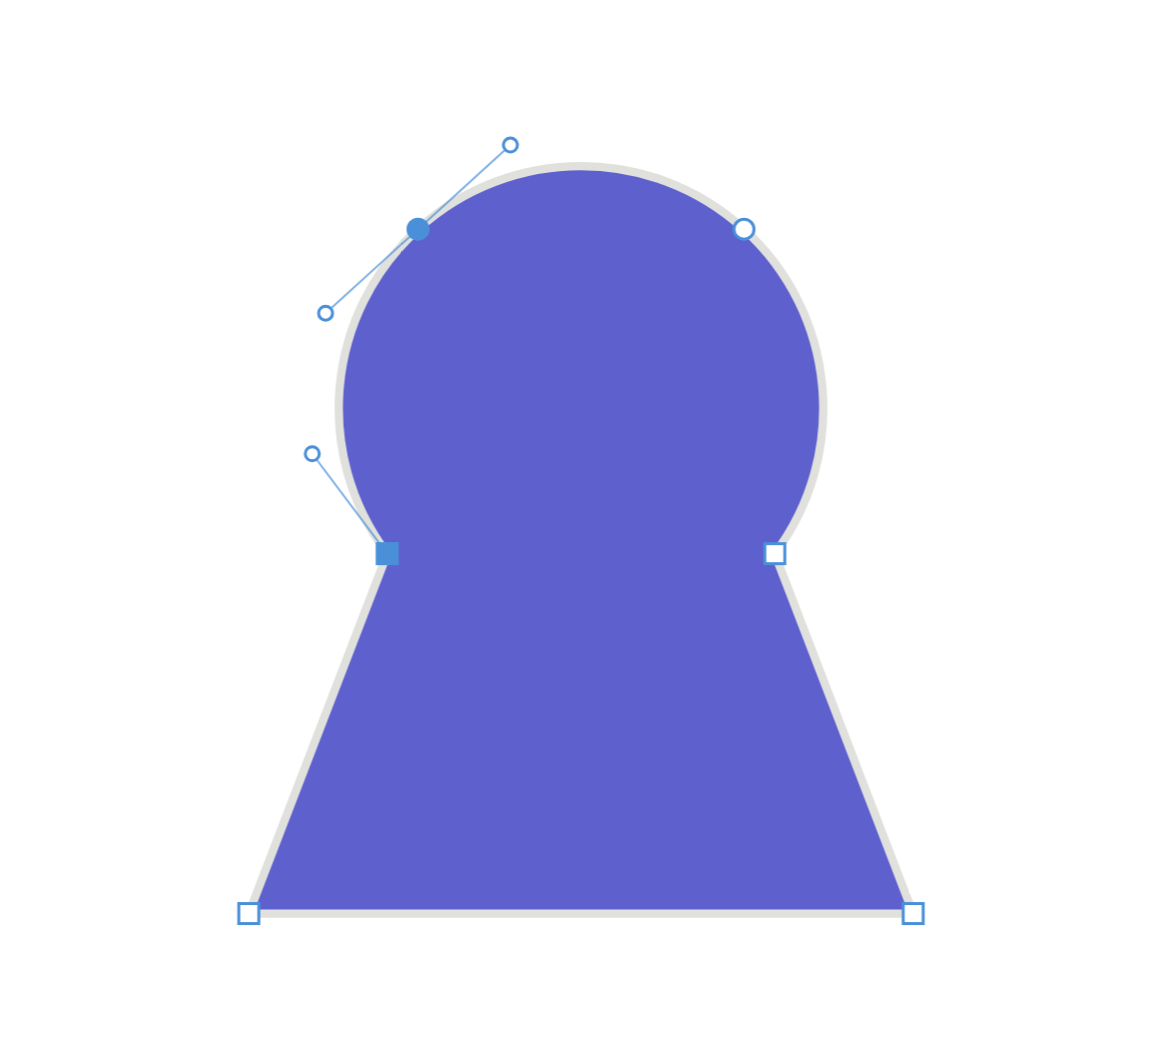
\includegraphics[width=0.5\textwidth]{images/editor/edit-nodes.png}
\caption{Két kijelölt csomópont a fogantyúival}
\label{fig:edit-nodes}
\end{figure}

A fogantyúk abszolút koordinátákként tárolódnak, nem a csomóponthoz viszonyított eltolásként. Az eltolás, a méretezés és a tükrözés emiatt minden pontra ugyanaz a leképezés, a csomópontokat és a fogantyúkat nem kell külön kezelni. Sima csomópontnál az egyik fogantyú mozgatása a másikat az ellenkező irányba igazítja, és a görbe törés nélkül halad át a csomóponton.

\section{Logikai műveletek és vágás}
\label{sec:boolean_impl}

A logikai műveletek a paper.js könyvtár \texttt{unite}, \texttt{subtract}, \texttt{intersect} és \texttt{exclude} metódusaira épülnek~\cite{paperjs}. A szerkesztő a kijelölt alakzatokat előbb paper.js útvonalakká alakítja. A téglalapok, ellipszisek és vonalak ehhez útvonallá válnak, a forgatás beépül a csomópontok koordinátáiba, a fogantyúk pedig a csomóponthoz viszonyított értékekre alakulnak, mert a paper.js ezt a formát várja. Az eredményt ugyanígy alakítja vissza.

A műveletek a halmozási sorrendet követik. Az unió, a metszet és a kizárás eredménye a legfelső alakzat stílusát kapja. A különbség a legalsó alakzatból vágja ki az összes többit, és a legalsó stílusát tartja meg. A felosztás minden alakzatot a körvonalaik által kijelölt darabokra bontja, és minden darab annak az alakzatnak a stílusát kapja, amelyik legfelül fedi. A paper.js dokumentációja szerint a felosztás egy különbség és egy metszet együttese~\cite{paperjs}. Több alakzatra a szerkesztő ezt lépésenként terjeszti ki. Minden következő alakzat az eddigi darabokat egy rajta kívüli és egy vele közös részre vágja, saját magából pedig az eddig le nem fedett rész lesz új darab. A felületen a műveletek \textit{Unite}, \textit{Subtract}, \textit{Intersect}, \textit{Exclude} és \textit{Divide} néven érhetők el. \Aref{fig:boolean}. ábra két egymást fedő alakzaton mutatja az öt műveletet.

\begin{figure}[!htbp]
\centering
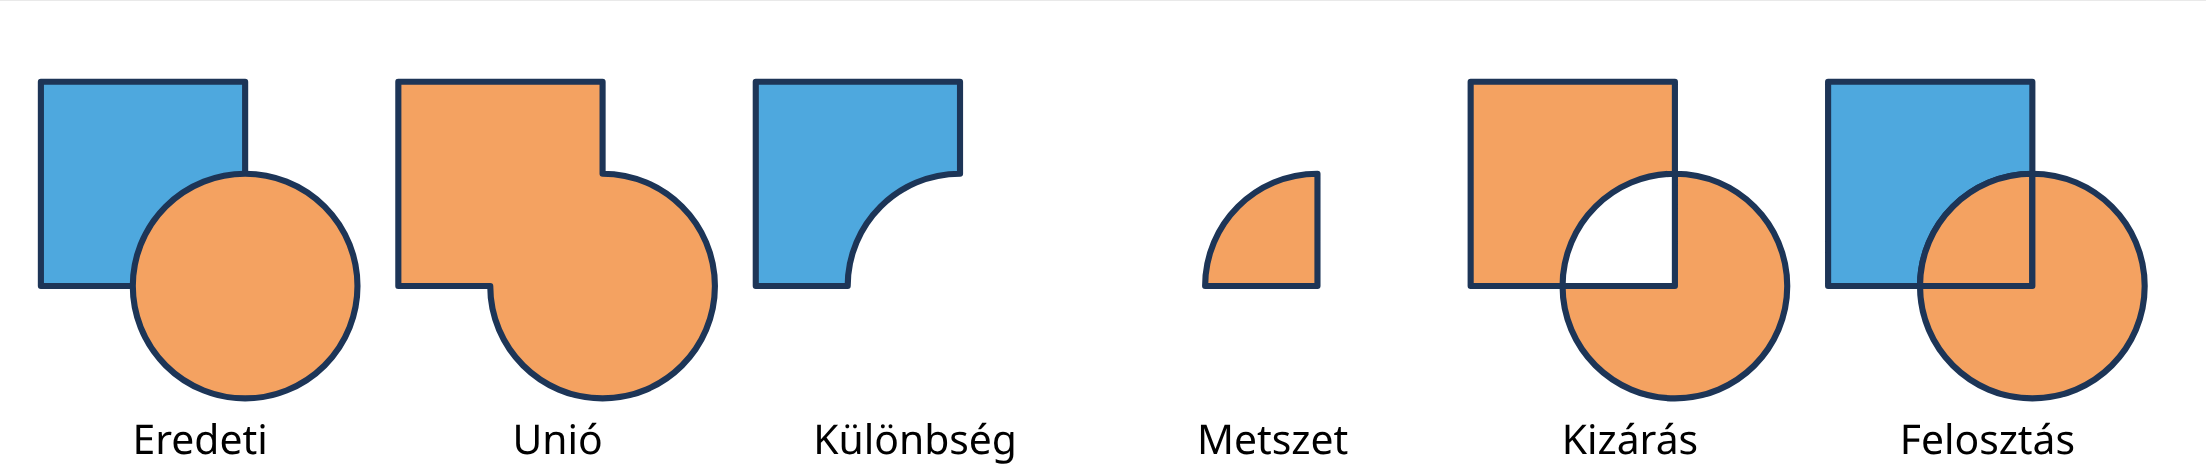
\includegraphics[width=\textwidth]{images/editor/boolean.png}
\caption{Két alakzat és a rajtuk végzett öt logikai művelet eredménye}
\label{fig:boolean}
\end{figure}

Az olló eszköz kétféleképpen vág. Egy kattintás az útvonal körvonalán csak abban a pontban vágja el az útvonalat: egy nyitott útvonal két részre esik, egy zárt útvonal pedig ott kinyílik. A vágás helyére új csomópont kerül, amelyet a de Casteljau-algoritmus számol ki~\cite{farin2002}, így az alakzat alakja nem változik. Egy húzás ezzel szemben kést rajzol, amely mentén minden eltalált alakzat kettéválik. Zárt alakzatnál a darabok is zártak, vagyis a körvonal a vágás mentén is végigfut.

Egy vonalnak nincs területe, ezért közvetlenül nem lehet logikai művelet operandusa. A szerkesztő a késből egy területet épít, ahogyan \aref{lst:knife}. programkód mutatja. A kés két végét az érintő irányában messzire meghosszabbítja, és a vonalat az egyik oldalán körbezárja. A darabok ezután egy metszet és egy különbség eredményeként állnak elő. Ha a felhasználó a kést a kiindulópontjáig visszahúzza, az lasszóként működik, és maga a zárt vonal lesz a vágó terület.

\begin{lstlisting}[style=TS, caption={A késből épített vágó terület (\texttt{utils/boolean.ts})}, label=lst:knife]
export function knifeRegion(paper: Paper, knife: Item, far: number): Item {
  const first = knife.firstSegment.point, last = knife.lastSegment.point;
  const t0 = knife.getTangentAt(0).normalize();
  const t1 = knife.getTangentAt(knife.length).normalize();
  const start = first.subtract(t0.multiply(far)), end = last.add(t1.multiply(far));
  const dir = end.subtract(start).normalize();
  const side = new paper.Point(-dir.y, dir.x).multiply(far * 2);
  const region = knife.clone({ insert: false });
  region.insert(0, start);
  region.add(end, end.add(side), start.add(side));
  region.closed = true;
  return region;
}
// the two pieces:  target.intersect(region)  and  target.subtract(region)
\end{lstlisting}

\section{Körvonalak}
\label{sec:strokes}

A körvonal beállításai közül a szaggatás és a körvonal útvonallá alakítása igényelt saját megoldást. Ez a szakasz ezeket és a velük rokon foltecsetet tárgyalja.

\subsection{Szaggatott vonalak}

Az SVG \texttt{stroke-dasharray} tulajdonsága abszolút hosszakat ír le~\cite{w3c-svg-painting}. Egy \texttt{6 4} minta vékony vonalon szaggatottnak látszik, egy 12 egység vastag, lekerekített végű vonalon viszont már folytonosnak, mert a vonalvégek kitöltik a hézagokat. A szerkesztő ezért a mintákat a vonalvastagsághoz viszonyítva kezeli. A szaggatott minta szakaszai a vastagság háromszorosai, a hézagai a kétszeresei, a pontozott minta pontjai pedig pontosan olyan hosszúak, amilyen vastag a vonal.

A lekerekített és a négyzetes vonalvég mindkét irányban a vastagság felével túlnyúlik a szakaszokon~\cite{w3c-svg-painting}. A szerkesztő ezt úgy egyenlíti ki, hogy a szakaszok hosszából levonja a vastagságot, a hézagokhoz hozzáadja, és a látható minta minden vonalvégnél ugyanolyan lesz. A pont ennek megfelelően egy majdnem nulla hosszú szakasz, amelyet a vonalvég tesz láthatóvá. Ha a felhasználó a vastagságot vagy a vonalvéget módosítja, a minta újraszámolódik. A kézzel beírt vagy importált minták viszont az SVG-hez hasonlóan abszolút értékek maradnak. Az exportált fájlban minden minta szabványos \texttt{stroke-dasharray} érték, amelyet bármely megjelenítő ugyanúgy rajzol ki.

\subsection{Körvonal útvonallá alakítása és a foltecset}

A körvonal útvonallá alakítása a kirajzolt körvonal területét kitöltött alakzattá teszi. Ehhez a görbét mindkét oldalán a vastagság felével el kell tolni, egy Bézier-görbe eltoltja azonban általában már nem Bézier-görbe, ezért csak közelíthető~\cite{elber1997}. A szerkesztő az útvonalat sűrűn, körülbelül másfél képpontonként mintavételezi, majd a Clipper könyvtár sokszögeltolásával a vonal mindkét oldalára kiterjeszti a vastagság felével, a vonalvég és a sarok beállítását is figyelembe véve~\cite{clipper}. Szaggatott vonalnál minden szakasz külön sokszög lesz. Az eredmény sokszögközelítés, amelyben az átfedések és a lyukak helyesen oldódnak fel. Egy apró eltérés azért marad, mert a hegyes sarkok korlátját túllépő csúcsokat a Clipper derékszögben vágja le, az SVG pedig ferdén.

A foltecset ugyanezt a technikát használja festésre. A húzás nyomvonalát az ecset méretére terjeszti ki, majd egyesíti azokkal a zárt alakzatokkal, amelyeket érint, és amelyeknek ugyanaz a kitöltése és körvonala. Az egyesített körvonalat a Ramer-Douglas-Peucker egyszerűsítés és a Catmull-Rom fogantyúk néhány sima csomóponttá alakítják, a hegyes sarkok azonban sarokpontok maradnak.

\section{Szövegek és betűtípusok}
\label{sec:text_impl}

A szöveg a szerkesztő legösszetettebb alakzata, mert a megjelenése a betűtípustól függ, amely a felhasználó gépén, a Google Fonts gyűjteményében vagy a szerkesztővel együtt szállítva is elérhető lehet. Az alábbiakban sorra veszem a szöveg szerkesztését, a betűtípusok forrásait és a szöveg útvonallá alakítását.

\subsection{Szövegszerkesztés és mérés}

A szöveg közvetlenül a vásznon szerkeszthető. Szerkesztés közben a szerkesztő egy \texttt{<textarea>} elemet helyez el egy \texttt{<foreignObject>} elemben, pontosan ott, ahol a szöveg megjelenik. Az Esc vagy a Ctrl+Enter billentyű, illetve egy máshová történő kattintás befejezi a szerkesztést.

A szöveg határoló téglalapjához ismerni kell a sorok szélességét. Ezt a böngésző vásznának \texttt{measureText} metódusa adja meg ugyanazzal a betűtípussal, amellyel a szöveg megjelenik, a betű- és szóközöket hozzászámolva. Egy webes betűtípus betöltése után a mérés eredménye megváltozhat, ezért a szerkesztő minden betöltött betűtípus után növel egy számlálót. A mérést végző reaktív kifejezések ettől a számlálótól függenek, és a kijelölő keret mindig a valódi szöveghez igazodik.

\subsection{Betűtípusok forrásai}

A betűtípusok három forrásból származhatnak. Az első a Google Fonts teljes gyűjteménye, amelyet a szerkesztő a CSS2 API-n keresztül ér el. Az API \texttt{text} paramétere esetén csak a felsorolt karaktereket tartalmazó, akár 90\%-kal kisebb fájlt ad vissza~\cite{google-fonts-css2}. A betűtípus-választóban ezért minden sor csak a betűtípus nevének betűit kéri le, és a lista görgetése néhány száz bájtos kérésekkel jár. Ha a kért stílus nem létezik a családban, az API az egész kérést elutasítja~\cite{google-fonts-css2}. A szerkesztő ezért a Fontsource metaadatai alapján csak a ténylegesen létező stílusokat kéri le~\cite{fontsource}, és ha mégis hiba történik, egy rövid visszalépési láncot követ, például félkövér dőltről félkövérre, majd normál dőltre.

A második forrás a felhasználó gépe. A Local Font Access API a felhasználó engedélyével felsorolja a telepített betűtípusokat, és hozzáférést ad a fájljaikhoz~\cite{mdn-local-fonts}. Ezt az API-t csak a Chromium-alapú böngészők valósítják meg. Más böngészőkben a szerkesztő néhány gyakori betűtípust a vásznon mért szélesség alapján ismer fel. Ezek megjeleníthetők, de útvonallá nem alakíthatók.

A harmadik forrás a szerkesztővel együtt szállított betűtípusok köre. A \texttt{serif}, a \texttt{sans-serif} és a többi általános CSS betűcsalád mögött minden böngészőben más betűtípus áll. A szerkesztő ezekhez nyílt licencű betűtípusokat tartalmaz~\cite{ofl}, és ezekkel jeleníti meg őket. A képernyőn látott szöveg és az útvonallá alakított változat így ugyanabból a betűtípusból készül. A fájlok írásrendszerenként külön részekre bontva töltődnek be, csak akkor, ha a szöveg tartalmazza az adott karaktereket.

\subsection{Szöveg útvonallá alakítása}

Az útvonallá alakításhoz a betűket ugyanúgy kell elrendezni, ahogyan a böngésző, vagyis azonos sorközzel, igazítással, betű- és szóközzel, alávágással és ligatúrákkal. Erre a fontkit könyvtár szolgál, amely teljes OpenType-szövegszedést végez~\cite{fontkit}. Az előbb kipróbált opentype.js könyvtár egyes betűtípusok alávágási tábláit nem tudta beolvasni, így a betűpárok távolsága eltért a böngészőben látottól. Egy Inter betűtípussal szedett mintaszövegen a képpontok mintegy 40\%-a eltért, ezért esett a választás a fontkit könyvtárra, amelynek pontosságát \aref{sec:text_accuracy}. alszakasz méri. Változó betűtípusoknál a szerkesztő a vastagság és az optikai méret tengelyét a szöveg beállításaira állítja. Ha a kért vastagság vagy dőlés nincs meg a betűtípusban, a böngészőkhöz hasonlóan mesterségesen állítja elő.

Az útvonallá alakításhoz szükség van a betűtípus fájljára. Google Fonts-betűtípusnál ez egy \texttt{text} paraméteres kérés, amely pontosan a szövegben szereplő karaktereket tartalmazó, kis méretű WOFF2-fájlt ad~\cite{google-fonts-css2,w3c-woff2}, helyi betűtípusnál pedig a Local Font Access API adja a fájlt. Ha a betűtípus egyik forrásból sem érhető el, a szerkesztő nem helyettesíti egy hasonlóval, hanem az okát megadva elutasítja az átalakítást. Egy csendes helyettesítés a felhasználó tudta nélkül változtatná meg a rajzot. A vegyesen jobbról balra és balról jobbra haladó szövegek kétirányú átrendezése nincs megvalósítva, ilyenkor az átalakítás figyelmeztet.

\section{SVG-importálás és -exportálás}
\label{sec:svg_io}

Az importálás egy idegen, akár hibás vagy rosszindulatú fájlt alakít a szerkesztő modelljére, az exportálás pedig a modellből szabványos fájlt készít. Az importálás dönti el, milyen fájlok és milyen korlátozásokkal szerkeszthetők, ezért ezt tárgyalom részletesebben.

\subsection{Importálás}

Az importálás a böngésző \texttt{DOMParser} objektumával kezdődik, amely az SVG-szöveget XML-dokumentummá alakítja. Ha az elemzés hibát jelez, vagy a gyökérelem nem \texttt{svg}, a szerkesztő elutasítja a fájlt. Az importáló ezután bejárja az elemfát, és minden támogatott elemből a szerkesztő saját alakzatát állítja elő. Közben nyilvántartja az egymásba ágyazott transzformációkat és az öröklődő stílusokat, mind a megjelenési attribútumokból, mind a \texttt{style} attribútumból. \Aref{tab:import}. táblázat összefoglalja, mit támogat az importáló, és mit nem.

\begin{table}[!htbp]
\caption{Az SVG-importáló által támogatott és nem támogatott szerkezetek}
\label{tab:import}
\centering
\footnotesize
\begin{tabular}{|>{\raggedright\arraybackslash}p{0.44\textwidth}|>{\raggedright\arraybackslash}p{0.44\textwidth}|}
\hline
\textbf{Támogatott} & \textbf{Nem támogatott vagy közelített} \\ \hline
\texttt{svg}, \texttt{g}, \texttt{a}, \texttt{use} a \texttt{defs} és \texttt{symbol} elemekkel; egymásba ágyazott transzformációk tetszőleges mátrixszal &
minták, amelyek szürke kitöltést kapnak \\ \hline
\texttt{switch}, amelyből az első olyan ág kerül át, amelynek feltételei, például a \texttt{systemLanguage}, teljesülnek &
\texttt{<style>} stíluslapok szabályai \\ \hline
\texttt{rect}, \texttt{circle}, \texttt{ellipse}, \texttt{line}, \texttt{polyline}, \texttt{polygon}, \texttt{path} minden paranccsal, \texttt{text} és \texttt{tspan} &
vágóútvonal, maszk, szűrő, jelölők (például nyílhegyek), keverési módok \\ \hline
megjelenési attribútumok és \texttt{style} attribútum öröklődéssel és az SVG alapértékeivel; \texttt{fill-opacity}, \texttt{stroke-opacity} &
útvonalra illesztett szöveg (\texttt{textPath}), \texttt{tref}, SVG-betűtípusok, animációk \\ \hline
\texttt{viewBox} méretezés; csoportok átlátszósága és forgatása &
nyírt képek és szövegek, amelyeket csak forgatás és méretezés közelít \\ \hline
lineáris és sugárirányú színátmenetek, \texttt{gradientTransform}, \texttt{href} láncok &
színátmenetek fókuszpontja és ismétlési módja \\ \hline
kitöltött összetett útvonalak nyitott és zárt részútvonalakkal &
körvonalas útvonal vegyes részútvonalai, amelyek külön alakzatokra válnak \\ \hline
\texttt{<image>} \texttt{data:} vagy \texttt{http(s)} címmel &
külön fájlra hivatkozó képek \\ \hline
\end{tabular}
\end{table}

A táblázat jobb oldali oszlopában szereplő szerkezetek közül egyik sem tűnik el szó nélkül. Minden kihagyott vagy közelített szerkezetről érthető üzenet szól, amelyet a szerkesztő az importálás után megjelenít, a felhasználó így pontosan tudja, mi változott a fájlon. Hogy ez valós fájlokon mennyire teljesül, azt \aref{sec:import_study}. alszakasz méri. A \texttt{script} és a \texttt{foreignObject} elem soha nem kerül át a szerkesztőbe, így egy importált fájl nem futtathat kódot. A bejárás legfeljebb negyven szint mélyre halad, és legfeljebb ötezer alakzatot hoz létre, egy szándékosan túlméretezett fájl így sem teheti használhatatlanná az oldalt. Ha a korlát miatt alakzatok maradnak ki, erről is figyelmeztetés szól.

A téglalapok, ellipszisek, vonalak és szövegek megtartják a típusukat, ha a rájuk ható transzformáció csak eltolás, méretezés és forgatás. Nyírás vagy tükrözés esetén útvonallá alakulnak, mert a modell ezeket csak útvonalként tudja pontosan ábrázolni. Az útvonalak elliptikus íveit az importáló az SVG implementációs függeléke szerint előbb középponti paraméterezésre alakítja~\cite{w3c-svg-implnote}, majd a körívekhez hasonlóan legfeljebb 90 fokos harmadfokú szakaszokkal közelíti.

\subsection{Exportálás}

Az exportált SVG szabványos dokumentum. A színátmenetek egy közös \texttt{<defs>} elembe kerülnek, az alakzatok pedig \aref{tab:shape-types}. táblázatban felsorolt elemekként jelennek meg. A koordináták két tizedesjegyre kerekítve íródnak ki, ami a képernyőn nem látható eltérést okoz, de jelentősen csökkenti a fájl méretét.

A szöveg háromféleképpen hagyhatja el a szerkesztőt. Maradhat egyszerű \texttt{<text>} elem, ekkor a megjelenítő gépen is telepítve kell lennie a betűtípusnak. A Google Fonts-betűtípusok \texttt{data:} URL formában be is ágyazhatók a fájlba~\cite{mdn-fontface}, mert egy URL-lel hivatkozott betűtípus nem töltődik be, ha az SVG képként vagy hálózat nélkül nyílik meg. Végül a szöveg útvonallá is alakítható, és akkor a fájlhoz semmilyen betűtípus nem kell. A helyi betűtípusok beágyazása külön választható, és figyelmeztetéssel jár, mert az ilyen betűtípusok licence gyakran tiltja a terjesztést.

A raszteres kép a dokumentum SVG változatából készül, amelyet a szerkesztő képként betölt, egy vászonra rajzol, majd PNG, JPG vagy WebP formátumban ment. A raszteres kép alapértelmezés szerint legalább 4000 képpont széles, hogy egy kis méretű lapról készült kép is éles legyen nagyobb kijelzőn vagy nyomtatásban. Az exportálás beállításaiban helyette méretarány vagy pontos szélesség is megadható. A vászon legnagyobb mérete böngészőnként és eszközönként eltér~\cite{mdn-canvas}, a szerkesztő ezért oldalanként legfeljebb 16\,384, összesen legfeljebb 268 millió képpontos képet készít, és ennél nagyobb méret kérésekor hibaüzenetet ad. Rajzolás előtt a szerkesztő a szövegeket útvonallá alakítja, hogy a kép ne függjön attól, hogy a képként betöltött SVG-ben a betűtípusok betöltődnek-e. Ha egy szöveg betűtípusa nem érhető el, például hálózat nélkül, a szöveg a böngésző betűtípusaival készül, és erről figyelmeztetés szól. Az SVG eleve a célméretben készül, a böngésző tehát a vektoros rajzot teljes felbontásban rajzolja ki, és nem egy kis képet nagyít fel.

\section{Vágólap és tárolás}
\label{sec:clipboard_storage}

A másolás egyszerre két helyre ír. A rendszer vágólapjára SVG-szövegként kerül a kijelölés, így más programokba, például az Inkscape-be vagy egy szövegszerkesztőbe is beilleszthető~\cite{mdn-clipboard}. Emellett a szerkesztő a kijelölt alakzatokat a böngésző helyi tárolójába is elmenti, amelyet ugyanannak az oldalnak minden lapja elér, az SVG-szöveget pedig egy erre a bejegyzésre hivatkozó XML megjegyzéssel jelöli meg. Beillesztéskor a következő sorrendben dönt:

\begin{enumerate}
\item a saját jelölésével ellátott SVG-szöveg esetén a tárolt alakzatok kerülnek vissza minden adatukkal, akár egy másik lapról is;
\item más programból származó SVG-szöveget az importálón keresztül, szerkeszthető alakzatokként illeszt be;
\item a vágólapon lévő kép képként kerül a rajzba;
\item ha a rendszer vágólapján nincs használható tartalom, a szerkesztő legutóbbi saját másolatát illeszti be.
\end{enumerate}

A projektfájl betöltésekor a szerkesztő minden alakzatot mezőnként ellenőriz. Az ismeretlen típusú vagy hiányos alakzatokat eldobja, a számokat, például a betűméretet, a megengedett tartományra szorítja, az ismétlődő azonosítókat lecseréli, és a csoportok mélységét is korlátozza. Egy kézzel szerkesztett vagy sérült fájl így nem okozhat hibát a szerkesztő többi részében. Az automatikus mentés a dokumentum minden változása után 800 ezredmásodperc szünettel írja a projektet a böngésző helyi tárolójába~\cite{whatwg-webstorage}. A betöltéskori állapotot nem menti, nehogy egy üres dokumentum felülírjon egy visszaállított munkát. Ha a tároló megtelt, a szerkesztő figyelmeztet, hogy a munkát fájlba kell menteni.

\section{Reszponzív felület és érintés}
\label{sec:touch}

A keskeny elrendezést egy \texttt{(max-width: 640px)} médialekérdezés kapcsolja be~\cite{mdn-media-queries}. Ugyanez a lekérdezés egy Svelte store-ban is elérhető, így a komponensek a viselkedésüket is hozzáigazíthatják, nem csak a stílusukat. Keskeny kijelzőn a tulajdonságpanel alulról nyíló lappá válik, a parancssávból pedig néhány ritkábban használt vezérlő, például az átlátszóság kimarad, amely a panelen továbbra is elérhető.

A szerkesztő az egér, a toll és az ujj eseményeit egységesen, a Pointer Events szabvány eseményeivel kezeli~\cite{w3c-pointer-events}. A vásznon a böngésző saját érintéses görgetését és nagyítását a \texttt{touch-action} CSS-tulajdonság kapcsolja ki~\cite{mdn-touch-action}, ezeket a mozdulatokat a szerkesztő maga dolgozza fel. Három helyen kellett külön megoldást keresni.

Az első a két ujjas nagyítás. Egy érintés nem jut el azonnal az aktuális eszközhöz, hanem 90 ezredmásodpercig vár. Ha ezalatt egy második ujj is a képernyőhöz ér, a mozdulat nagyítás, és az eszköz egyáltalán nem értesül az első ujjról. E várakozás nélkül a toll minden nagyítás előtt egy felesleges csomópontot helyezne el. Nagyítás közben az ujjak közötti pont a helyén marad, és ha a két ujj együtt mozog, a nézet követi őket.

A második a helyi menü. Az iOS Safari böngésző nem küldi el a \texttt{contextmenu} eseményt, ezért a szerkesztő saját hosszú érintést valósít meg. Ha az ujj 550 ezredmásodpercig egy helyben marad, megnyílik a helyi menü.

A harmadik a fogantyúk mérete. Ha a fő mutatóeszköz az ujj, a fogantyúk és a csomópontok egy láthatatlan, 14 képpont sugarú, vagyis 28 képpont átmérőjű érzékeny területet kapnak. A WCAG 2.2 irányelv 2.5.8-as sikerkritériuma legalább 24 × 24 CSS-képpontos célméretet ír elő~\cite{wcag-target-size}, ennek a szerkesztő fogantyúi megfelelnek. Parhi és társai vizsgálatában a hüvelykujjal használt telefonon a 9,2-9,6 mm-es célok voltak megbízhatóan eltalálhatók~\cite{parhi2006}. A 28 képpont a CSS 96 dpi-s névleges felbontásán körülbelül 7,4 mm, a fogantyúk tehát ennél kisebbek, cserébe sűrűn elhelyezkedő csomópontok mellett is külön-külön megfoghatók maradnak.

Hasonló kérdést vetett fel az objektumok panel. Az elemek ott húzással rendezhetők, érintőképernyőn azonban ugyanez a mozdulat a lista görgetését is jelentheti. A húzás ezért csak akkor kezdődik, ha az ujj 150 ezredmásodpercig egy helyben maradt, különben a mozdulat görgetésnek számít.

\chapter{Tesztelés és használat}
\label{ch:test}

A fejezet első fele a szerkesztő ellenőrzésének módját mutatja be, a második fele az elkészült alkalmazás használatát.

\section{Tesztelési stratégia}
\label{sec:test_strategy}

A tesztelés \aref{sec:architecture}. szakaszban leírt rétegeket követi. Minél lejjebb van egy kódrészlet a rétegek között, annál egyszerűbb és gyorsabb tesztelni, ezért a tesztek többsége az alsó rétegekre irányul. A geometriai számításokat, az útvonalak feldolgozását, a színértékek értelmezését, az SVG-importálást és -exportálást a tesztek közvetlenül, bemenetek és elvárt kimenetek alapján ellenőrzik.

Az eszközök tesztjei mesterséges \texttt{PointerInfo} eseményeket küldenek, majd a dokumentum és az előzmények állapotát vizsgálják. Egy téglalap rajzolásának tesztje például egy lenyomást, néhány mozgatást és egy felengedést ad át a téglalap eszköznek, és ellenőrzi, hogy pontosan egy új alakzat és egy új előzménybejegyzés keletkezett. A felület részeit, a vásznat, a paneleket, a színválasztót és a párbeszédablakokat, végül a teljes alkalmazást a tesztek a jsdom környezetében jelenítik meg~\cite{jsdom}, és DOM-eseményekkel kezelik.

A jsdom nem végez valódi elrendezést és megjelenítést, így például az elemek mérete és a szöveg szélessége nem mérhető vele. Ezeket a tesztek egyszerű közelítéssel helyettesítik, a valódi megjelenést pedig böngészőben ellenőriztem. Az automatikus teszteket valódi böngészőben végzett kézi tesztelés egészítette ki, és az ennek során talált hibákhoz a javítás előtt egy-egy automatikus teszt készült.

\section{Automatikus tesztek}
\label{sec:unit_tests}

A tesztek a Vitest keretrendszerrel futnak~\cite{vitest}, a \texttt{tests} mappában, témák szerint öt almappába rendezve. A tesztek témakörök szerinti megoszlása \aref{tab:tests}. táblázatban látható.

\begin{table}[!htbp]
\caption{Az automatikus tesztek elosztása}
\label{tab:tests}
\centering
\footnotesize
\begin{tabular}{|l|>{\raggedright\arraybackslash}p{0.52\textwidth}|r|r|}
\hline
\textbf{Mappa} & \textbf{Témakör} & \textbf{Fájl} & \textbf{Teszteset} \\ \hline
\texttt{model} & alakzatok, útvonalak, csoportok, színátmenetek, szaggatás, előzmények, projektfájl, beállítások, véletlenszerű tesztek & 12 & 114 \\ \hline
\texttt{tools} & rajzolás, kijelölés, csomópontok, illesztés, logikai műveletek, olló, foltecset & 7 & 71 \\ \hline
\texttt{io} & SVG-importálás és -exportálás, raszteres export, képek, vágólap & 6 & 64 \\ \hline
\texttt{fonts} & Google Fonts kérések, helyi betűtípusok, beágyazás, szöveg útvonallá alakítása, betűtípus-választó & 7 & 79 \\ \hline
\texttt{ui} & vászon, panelek, színválasztó, párbeszédablakok, nézet, teljes alkalmazás, regressziós tesztek & 8 & 81 \\ \hline
\textbf{Összesen} & & \textbf{40} & \textbf{409} \\ \hline
\end{tabular}
\end{table}

A forráskódban 409 teszteset szerepel. Futtatáskor a keretrendszer 447 tesztet jelez, mert a véletlenszerű tesztek egyik tesztesete negyven különböző kezdőértékkel fut le. A teljes tesztkészlet egy átlagos fejlesztői gépen 30-40 másodperc alatt fut le, és minden módosítás után könnyen lefuttatható. \Aref{tab:req-tests}. táblázat azt mutatja, mely tesztfájlok ellenőrzik \aref{tab:requirements}. táblázat követelményeit.

\begin{table}[!htbp]
\caption{A funkcionális követelmények és az őket ellenőrző tesztfájlok}
\label{tab:req-tests}
\centering
\footnotesize
\renewcommand{\arraystretch}{1.15}
\begin{tabular}{|l|>{\raggedright\arraybackslash}p{0.2\textwidth}|>{\raggedright\arraybackslash}p{0.6\textwidth}|}
\hline
\textbf{Az.} & \textbf{Terület} & \textbf{Tesztfájlok} \\ \hline
F1 & Elrendezés & \texttt{ui/app}, \texttt{ui/panels}, böngészős ellenőrzés \\ \hline
F2 & Rajzolás & \texttt{tools/drawing}, \texttt{ui/canvas} \\ \hline
F3 & Tulajdonságok & \texttt{model/shapes}, \texttt{tools/select}, \texttt{ui/panels} \\ \hline
F5 & Szöveg & \texttt{fonts/text}, \texttt{fonts/outline}, \texttt{fonts/textOutline}, \texttt{ui/canvas} \\ \hline
F6 & Színek & \texttt{model/gradient}, \texttt{model/dash}, \texttt{ui/color-picker} \\ \hline
F7 & Útvonalak & \texttt{model/path}, \texttt{model/strokeToPath}, \texttt{tools/edit}, \texttt{tools/boolean}, \texttt{tools/scissors} \\ \hline
F8 & Illesztés, igazítás & \texttt{tools/snap} \\ \hline
F9 & Objektumok & \texttt{model/groups}, \texttt{model/lock} \\ \hline
F10 & Kijelölés & \texttt{tools/select}, \texttt{ui/canvas-tools} \\ \hline
F11 & Vágólap & \texttt{io/clipboard} \\ \hline
F12 & Nagyítás & \texttt{ui/view}, böngészős ellenőrzés \\ \hline
F13 & Visszavonás & \texttt{model/history}, \texttt{model/fuzz} \\ \hline
F14 & Mentés & \texttt{model/project}, \texttt{model/preferences} \\ \hline
F15 & Import, export & \texttt{io/import}, \texttt{io/serializer}, \texttt{io/export}, \texttt{io/images}, \texttt{fonts/embed} \\ \hline
\end{tabular}
\end{table}

\newpage

Néhány jellemző eset a tesztek közül:

\begin{itemize}
\item egy elforgatott téglalap importálás után elforgatott téglalap marad, egy nyírt téglalap viszont útvonallá alakul;
\item egy csoport exportálás és újbóli importálás után is megtartja a forgatását és az átlátszóságát;
\item két kör egyesítése néhány görbe csomópontot ad, nem sokszöget;
\item a szöveg útvonallá alakításakor az ,,o'' betű két kontúrt kap, egy külsőt és egy belső lyukat, a magyar ,,ő'' és ,,ű'' betű pedig helyesen jelenik meg;
\item egy ismeretlen betűtípusú szöveget a szerkesztő nem alakít útvonallá, a szöveg szöveg marad.
\end{itemize}

\section{Véletlenszerű tesztelés}
\label{sec:fuzz}

A kézzel írt tesztek azokat az eseteket ellenőrzik, amelyekre a fejlesztő gondolt. A szerkesztőben viszont a műveletek tetszőleges sorrendben követhetik egymást, és egyes hibák csak ritka kombinációkban jelentkeznek, például egy csoportba belépve, egy forgatás és egy visszavonás után. Ezek felderítésére véletlenszerű műveletsorozatokat végrehajtó teszt készült, angol nevén \textit{fuzzing}. A módszer Miller és társai 1990-es vizsgálatából ered, amelyben véletlenszerű bemenettel a UNIX-segédprogramok negyedét-harmadát sikerült összeomlasztani~\cite{miller1990}.

A teszt egy kezdőértékkel inicializált álvéletlenszám-generátor alapján súlyozottan választ a műveletek közül. Alakzatokat rajzol az eszközökkel, mozgat, méretez, forgat, csoportosít, csoportba lép be, csomópontokat szerkeszt, stílust módosít, visszavon és megismétel. Az ellenőrzés a QuickCheck eszközzel ismertté vált tulajdonságalapú tesztelést követi~\cite{claessen2000}, vagyis nem egy konkrét kimenetet vár, hanem olyan állításokat, amelyeknek minden állapotban igaznak kell lenniük. Minden lépés után néhány olcsón ellenőrizhető tulajdonságot vizsgál, például hogy a kijelölés pontosan a belépett csoport szintjén lévő alakzatokra vonatkozik. Néhány lépésenként és a futás végén költségesebb ellenőrzések is lefutnak:

\begin{itemize}
\item a projektfájlba mentett, majd visszatöltött dokumentum ugyanazokat az alakzatokat adja ugyanott
\item az exportált SVG minden útvonal csomópontjait tartalmazza
\item az összes lépés visszavonása után a kiinduló dokumentum áll vissza
\end{itemize}

Alapértelmezés szerint negyven kezdőérték fut le, egyenként százötven lépéssel, és egy további futás hétszáz lépéssel, amely túllépi az előzmények kétszáz lépéses korlátját. Hiba esetén a teszt kiírja a kezdőértéket és az utolsó műveleteket, a hibás sorozat tehát pontosan megismételhető.

\section{Betűtípusok tesztelése hálózat nélkül}
\label{sec:fake_google}

A betűtípusokkal kapcsolatos kód nagy része a Google Fonts és a Fontsource szolgáltatásainak küld kéréseket. A tesztek nem használhatják a valódi hálózatot, mert akkor lassúak és megbízhatatlanok lennének. Egy segédmodul ezért helyettesíti a szolgáltatásokat, és ott, ahol ez számít, a valódi API viselkedését utánozza. Egy nem létező stílus kérését az egész kérés elutasításával válaszolja meg, a \texttt{text} paraméteres kérésre egyetlen \texttt{@font-face} blokkot ad, a paraméter nélküli kérésre pedig írásrendszerenként egyet~\cite{google-fonts-css2}. Betűtípusfájlként a tesztkészletben tárolt kis betűtípusfájlokat küldi vissza.

\section{Kézi tesztelés és regressziós tesztek}
\label{sec:manual_tests}

A kézi tesztelés során a felület minden részét végigpróbáltam, és a talált hibákat egy hibalistába gyűjtöttem. A hibák egy része csak a komponensek együttműködésében jelentkezett, ezért a hozzájuk tartozó tesztek a teljes vásznat jelenítik meg. \Aref{tab:regressions}. táblázat a hibalista néhány jellemző bejegyzését és a hozzájuk tartozó teszteket mutatja. A tesztek neve a hiba azonosítójával kezdődik, egy hiba újbóli megjelenése tehát azonnal azonosítható.

\begin{table}[!htbp]
\caption{Hibák a kézi tesztelésből és a hozzájuk tartozó regressziós tesztek}
\label{tab:regressions}
\centering
\footnotesize
\begin{tabular}{|l|>{\raggedright\arraybackslash}p{0.78\textwidth}|}
\hline
\textbf{Azonosító} & \textbf{A teszt által ellenőrzött viselkedés} \\ \hline
B-01 & Az exportált SVG jól formált XML, és nem függ külső betűtípustól. \\ \hline
B-02 & Egy csomópont húzása közben a csomópontok és a fogantyúk a görbével együtt mozognak. \\ \hline
B-03 & A toll eszközzel az első pontra lenyomva és húzva kattintásként viselkedik, a későbbi pontok viszont sima csomóponttá húzhatók. \\ \hline
B-04 & Az útvonal bezárásának előnézete pontosan azt az alakzatot mutatja, amelyet a kattintás létrehoz. \\ \hline
B-05 & Rajzolás és kijelölés után a mozgatás, a méretezés és a forgatás a kijelölő keretet is mozgatja. \\ \hline
B-06 & A kijelölés megszüntetése, legyen az kattintás az üres vászonra, Esc vagy dupla kattintás, eltünteti a kijelölő keretet. \\ \hline
\end{tabular}
\end{table}

\section{Böngészős ellenőrzés és a kész alkalmazás mérete}
\label{sec:browser_check}

A fejlesztés során az alkalmazást folyamatosan egy Chromium-alapú asztali böngészőben használtam, a kézi tesztelés is ott történt. A jsdom által nem vizsgálható viselkedés, például a valódi elrendezés, a szöveg mérése, a raszteres export és az érintéses mozdulatok ellenőrzésének egy részét a Playwright eszközzel szkriptekbe foglaltam~\cite{playwright}. A Playwright programból vezérel egy Chromium böngészőt, asztali és telefonos képernyőméretre is beállítható, és érintéses eseményeket is küldhet. A dolgozat képernyőképei is így készültek. A felületet Firefox böngészőben is kipróbáltam, ott is helyesen működik, Safari böngészőben azonban nem teszteltem. A helyi betűtípusok elérése a Chromium-alapú böngészőkre korlátozódik, ezt \aref{sec:text_impl}. szakasz tárgyalja.

Az éles változatot a Vite csomagolja. A keletkező fő JavaScript-fájlokat \aref{tab:bundle}. táblázat sorolja fel. A nagy könyvtárak dinamikus importtal külön fájlba kerülnek, és csak az első használatukkor töltődnek be: a paper.js az első logikai műveletnél vagy vágásnál, a fontkit és a WOFF2 kibontó az első útvonallá alakításnál. Az alkalmazás indulásakor ezért csak a fő fájlt kell letölteni, amely tömörítve körülbelül 160 kB.

\begin{table}[!htbp]
\caption{Az éles változat fő JavaScript-fájljai}
\label{tab:bundle}
\centering
\footnotesize
\begin{tabular}{|l|l|r|r|}
\hline
\textbf{Fájl} & \textbf{Tartalom} & \textbf{Méret} & \textbf{Tömörítve} \\ \hline
\texttt{index} & a szerkesztő kódja & 504,2 kB & 160,8 kB \\ \hline
\texttt{paper-core} & paper.js & 318,9 kB & 112,3 kB \\ \hline
\texttt{browser-module} & fontkit & 363,0 kB & 150,5 kB \\ \hline
\texttt{decompress} & WOFF2 kibontó & 295,2 kB & 127,0 kB \\ \hline
\end{tabular}
\end{table}

\section{Az alkalmazás használata}
\label{sec:usage}

Indításkor az alkalmazás a legutóbbi automatikus mentést tölti vissza, ennek hiányában üres lappal nyílik meg. \Aref{fig:ui-main}. ábra a szerkesztőt asztali képernyőn mutatja. A rajzon egy kijelölt kör látható a nyolc méretező fogantyúval, a felette lévő forgató fogantyúval és a közepén a forgatási középponttal. A jobb oldali kitöltés panelen a kör sugárirányú színátmenete szerkeszthető. A színátmenet sávja alatt a színpontok, alattuk a színválasztó, legalul pedig az átmenet középpontja és sugara látható.

\begin{figure}[!htbp]
\centering
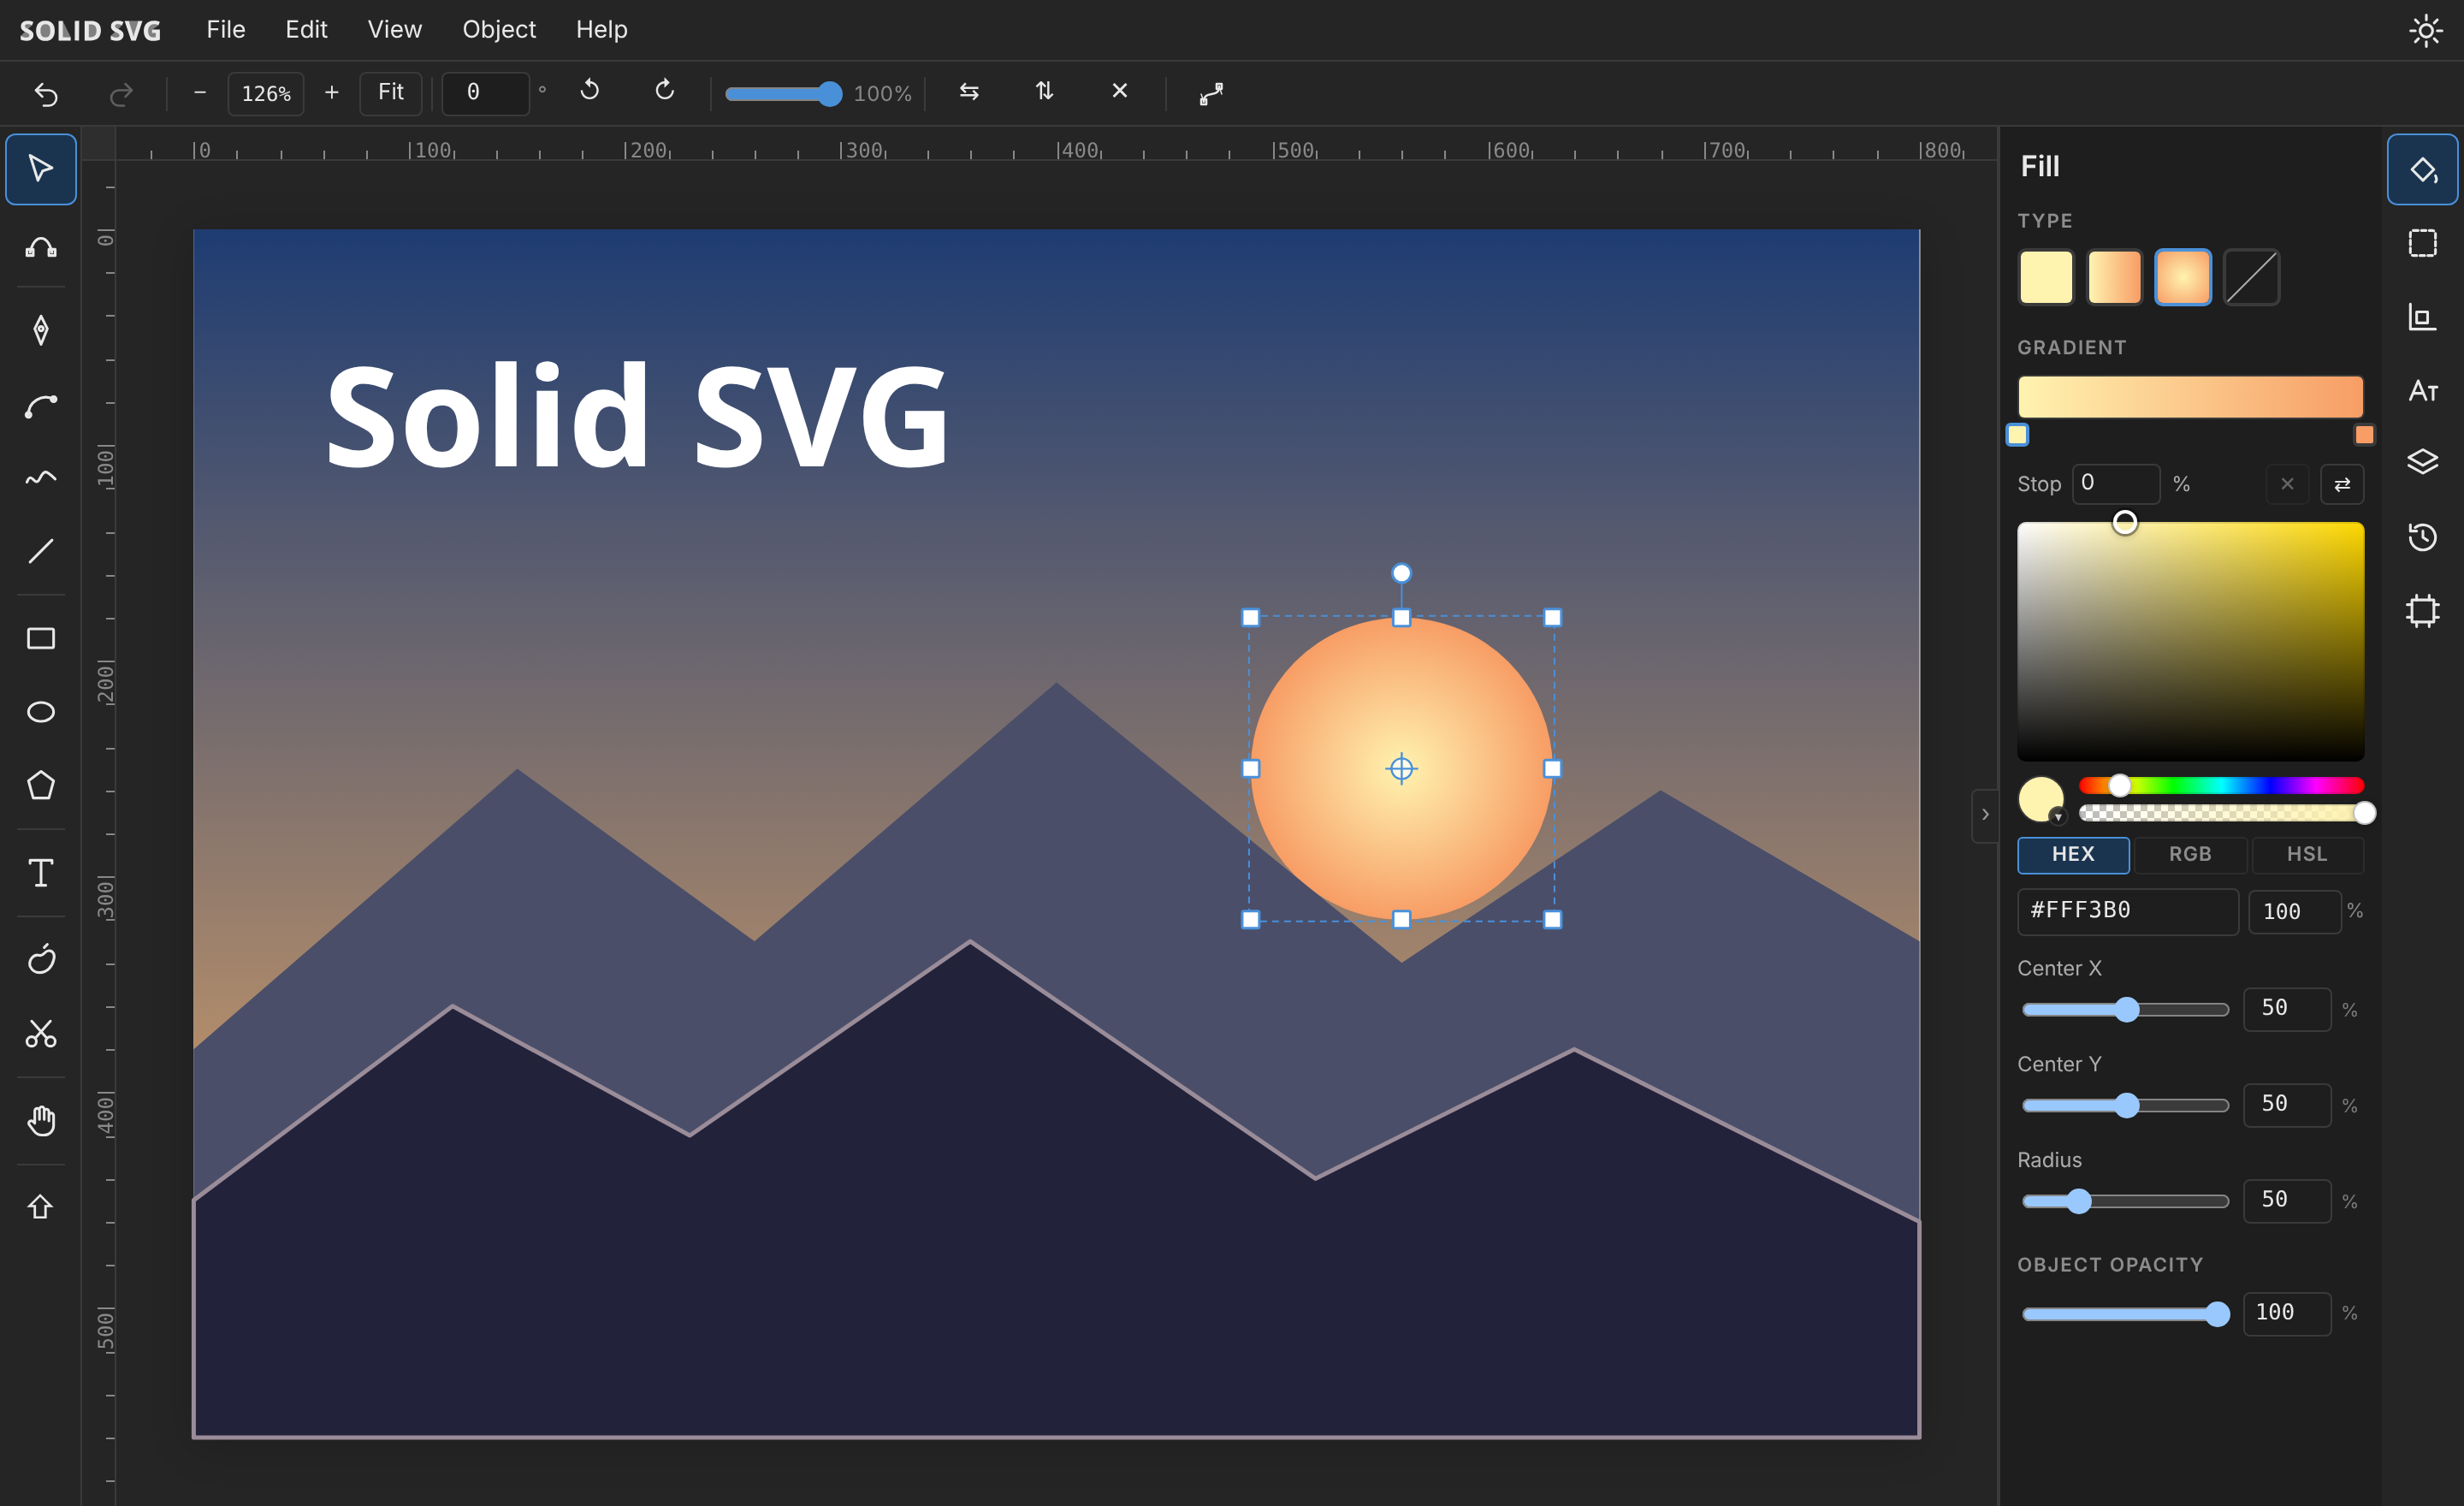
\includegraphics[width=\textwidth]{images/editor/ui-main.png}
\caption{A szerkesztő felülete asztali képernyőn, egy kijelölt alakzattal és a kitöltés panellel}
\label{fig:ui-main}
\end{figure}

\paragraph{Rajzolás.} Az eszköz a bal oldali eszköztárról vagy a billentyűjével választható ki. A téglalap, az ellipszis és a vonal húzással rajzolható, Shift billentyűvel négyzet, kör, illetve 45 fokos lépésekben elforgatott vonal készül. A sokszög eszköz kattintásonként egy csúcsot ad hozzá, a toll és a körív \aref{sec:drawing_tools}. szakaszban leírtak szerint működik. A szöveg eszközzel a vászonra kattintva közvetlenül lehet gépelni. Az eszközök billentyűit \aref{tab:tool-keys}. táblázat foglalja össze.

\begin{table}[!htbp]
\caption{Az eszközök és billentyűik}
\label{tab:tool-keys}
\centering
\footnotesize
\begin{tabular}{|l|c||l|c||l|c|}
\hline
\textbf{Eszköz} & \textbf{Bill.} & \textbf{Eszköz} & \textbf{Bill.} & \textbf{Eszköz} & \textbf{Bill.} \\ \hline
Kijelölés & V & Szabadkézi rajz & F & Szöveg & T \\ \hline
Csomóponteszköz & E & Vonal & L & Foltecset & Shift+B \\ \hline
Toll & B & Téglalap & R & Olló & C \\ \hline
Körív & A & Ellipszis & O & Nézet mozgatása & H \\ \hline
 & & Sokszög & P & & \\ \hline
\end{tabular}
\end{table}

\paragraph{Objektumok és geometria.} Az objektumok panel, a felületen \textit{Objects}, a dokumentum fáját mutatja, ez látható \aref{fig:panels}. ábra bal oldalán. Minden sorban ott van az alakzat típusának ikonja, a neve és a kitöltése, a kijelölt sorban pedig a zárolás és az elrejtés gombja is. A sorok húzással rendezhetők, és egy sort egy csoportra húzva az alakzat a csoportba kerül. Az ábra közepén a geometria panel, a felületen \textit{Geometry}, a pozíciót, a méretet, a forgatási középpontot és a forgatást mutatja. A forgatási középpont a határoló téglalap százalékában vagy a mellette lévő kilenc pont egyikével adható meg. Az ábrán a bal alsó sarokba került, a kijelölt hegyek tehát a bal alsó sarkuk körül fordulnának el.

\begin{figure}[!htbp]
\centering
\begin{minipage}[b]{0.31\textwidth}\centering
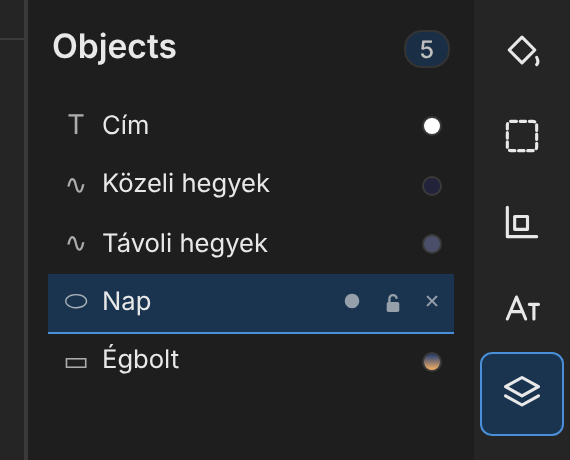
\includegraphics[width=\textwidth]{images/editor/ui-objects.png}\\[2pt]
{\footnotesize Objektumok panel}
\end{minipage}\hfill
\begin{minipage}[b]{0.31\textwidth}\centering
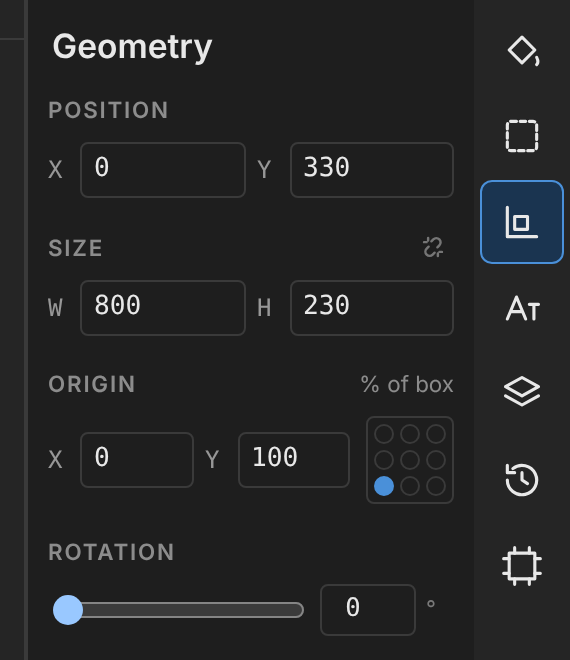
\includegraphics[width=\textwidth]{images/editor/ui-geometry.png}\\[2pt]
{\footnotesize Geometria panel}
\end{minipage}\hfill
\begin{minipage}[b]{0.33\textwidth}\centering
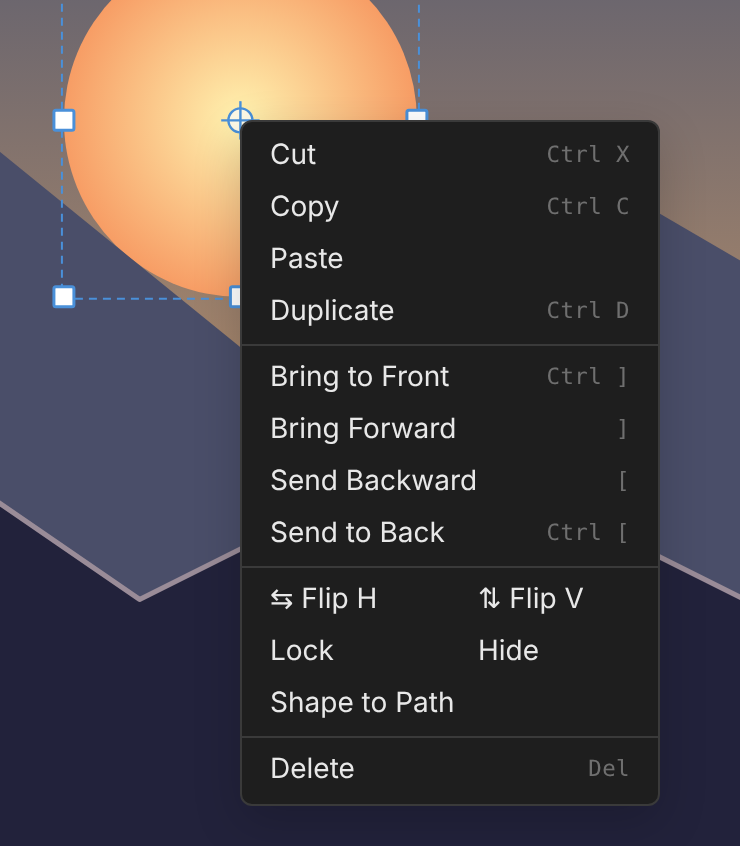
\includegraphics[width=\textwidth]{images/editor/ui-context-menu.png}\\[2pt]
{\footnotesize Helyi menü}
\end{minipage}
\caption{Az objektumok panel, a geometria panel és egy alakzat helyi menüje}
\label{fig:panels}
\end{figure}

\paragraph{Helyi menü.} Egy alakzatra jobb egérgombbal kattintva vagy érintőképernyőn hosszan megérintve megjelenik a helyi menü, \aref{fig:panels}. ábra jobb oldalán. A menüben csak az adott helyzetben elérhető műveletek szerepelnek: a vágólap műveletei, a sorrend módosítása, a tükrözés, a zárolás, az elrejtés, az útvonallá alakítás és a törlés. A billentyűkombinációk a menüpontok mellett is láthatók.

\paragraph{Mentés és exportálás.} A \textit{File} menü kínálja az új dokumentumot, a projekt vagy SVG-fájl megnyitását, a projekt mentését, SVG-fájlok és képek beillesztését a meglévő rajzba, valamint az exportálást SVG és raszteres formátumba. Az exportálás beállításai külön párbeszédablakban adhatók meg, amelyet \aref{fig:export}. ábra mutat. Itt választható ki, hogy a lap vagy csak a rajzolt alakzatok környezete kerüljön a fájlba, hogy a háttér is része legyen-e, és hogy a szöveg \aref{sec:svg_io}. szakaszban leírt módok közül melyikkel hagyja el a szerkesztőt. A raszteres képek mérete és minősége is itt állítható.

\paragraph{Telefonon.} Keskeny kijelzőn a felület \aref{fig:mobile}. ábrán látható módon rendeződik át. A tulajdonságpanel a vászon alatt jelenik meg, az eszköztár és a tulajdonságsáv a két oldalon marad. Az eszköztár alján lévő nyíl gomb a Shift billentyűt helyettesíti, bekapcsolva például a téglalap eszköz négyzetet rajzol, és a kijelölés bővíthető. A nézet két ujjal nagyítható és mozgatható.

{\restylefloat*{figure}
\begin{figure}[!htbp]
\centering
\begin{minipage}[b]{0.46\textwidth}\centering
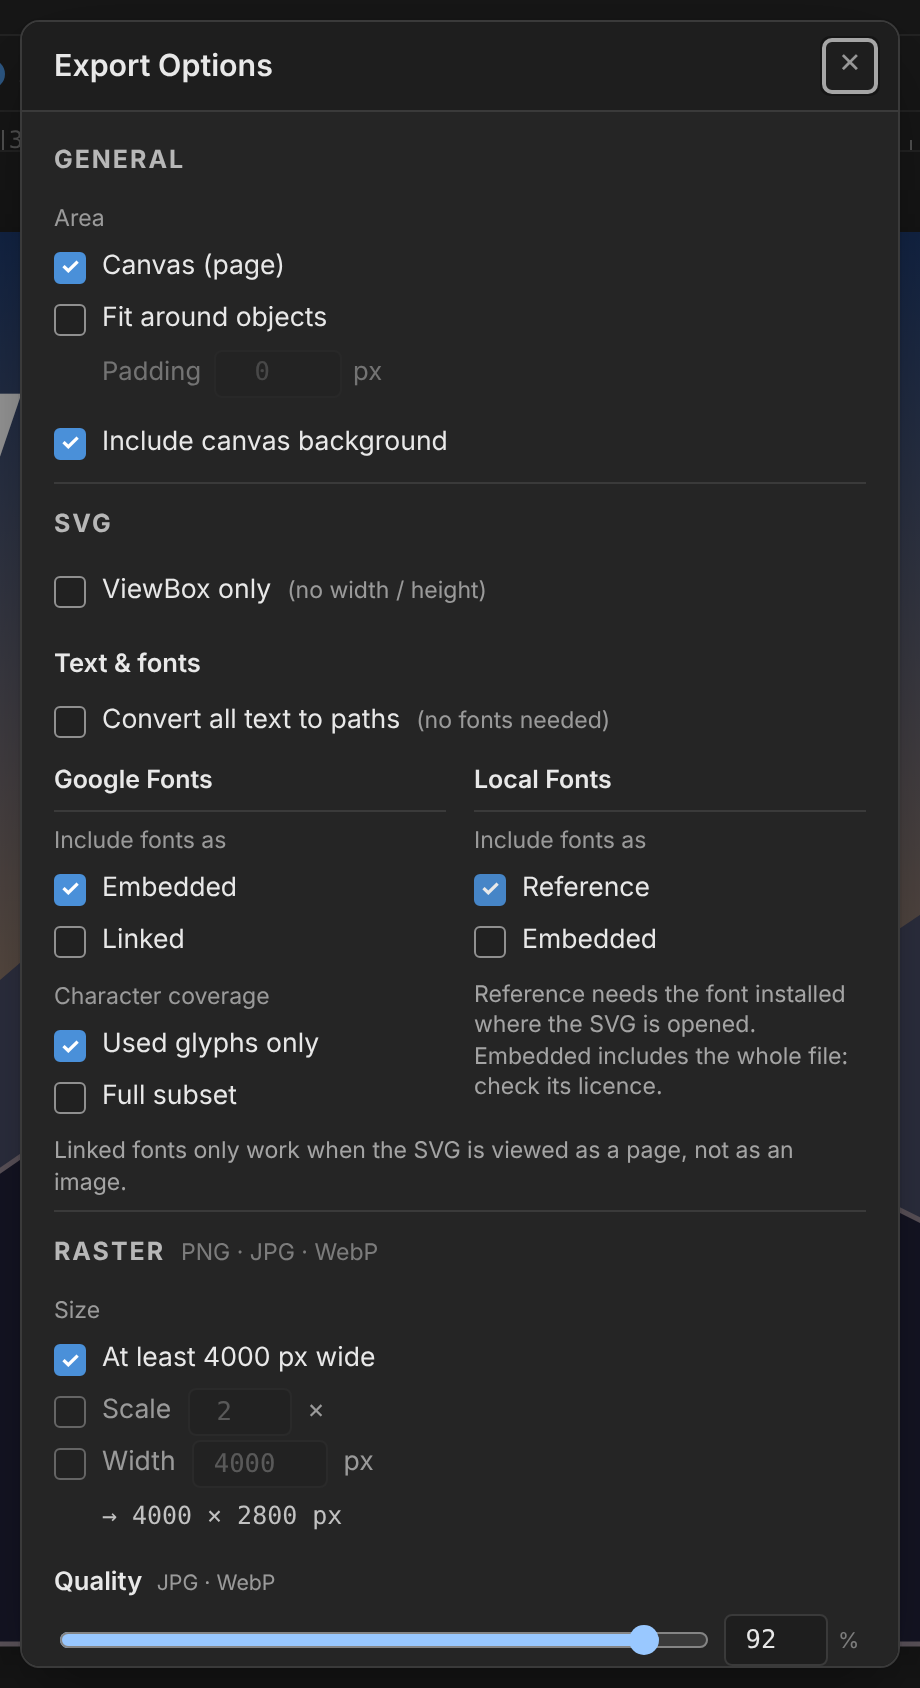
\includegraphics[height=0.5\textheight]{images/editor/ui-export.png}
\caption{Az exportálási beállítások párbeszédablakja}
\label{fig:export}
\end{minipage}\hfill
\begin{minipage}[b]{0.46\textwidth}\centering
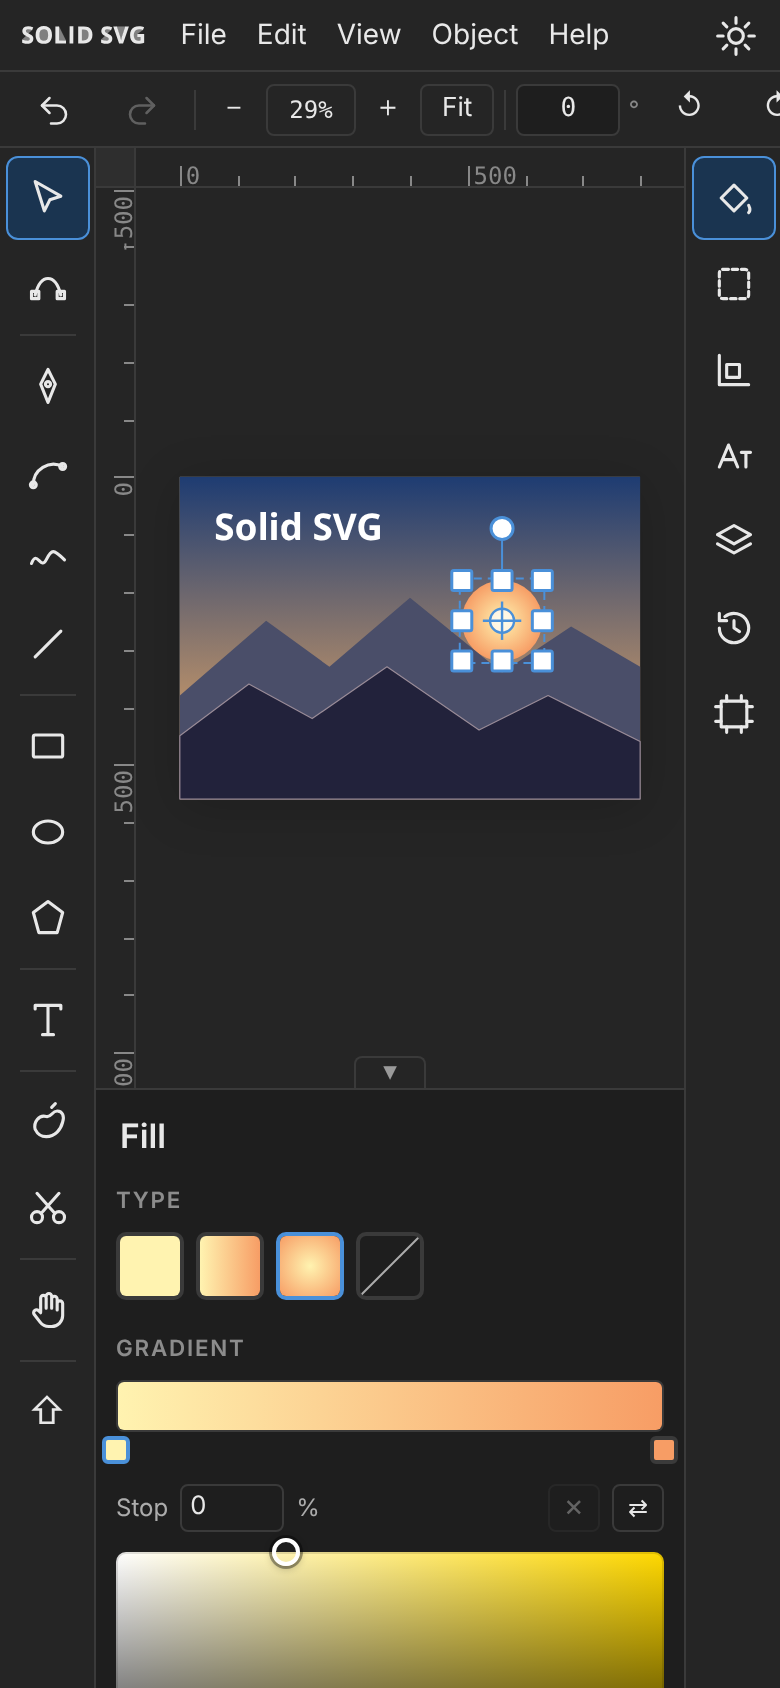
\includegraphics[height=0.5\textheight]{images/editor/ui-mobile.png}
\caption{A szerkesztő telefonon, nyitott tulajdonságpanellel}
\label{fig:mobile}
\end{minipage}
\end{figure}  
}
\chapter{Az eredmények értékelése}
\label{ch:evaluation}

Ez a fejezet azt vizsgálja, mennyiben teljesültek \aref{sub:editor_conclusions}. alszakasz célkitűzései és \aref{sec:requirements}. szakasz követelményei, mit mutatnak a két legfontosabb funkció mérései, hogyan viszonyul az elkészült szerkesztő \aref{sec:svg_editors}. szakaszban vizsgált alkalmazásokhoz, és milyen nem várt tapasztalatokkal járt a fejlesztés.

\section{A követelmények teljesülése}
\label{sec:req_fulfilment}

\Aref{tab:fulfilment}. táblázat a funkcionális követelmények teljesülését foglalja össze. A követelmények többsége teljesült, kettő részben, a korlátozásokat a megjegyzés oszlop nevezi meg.

\begin{table}[!ht]
\caption{A funkcionális követelmények teljesülése}
\label{tab:fulfilment}
\centering
\footnotesize
\renewcommand{\arraystretch}{1.15}
\begin{tabular}{|l|>{\raggedright\arraybackslash}p{0.2\textwidth}|l|>{\raggedright\arraybackslash}p{0.47\textwidth}|}
\hline
\textbf{Az.} & \textbf{Terület} & \textbf{Teljesülés} & \textbf{Megjegyzés} \\ \hline
F1 & Elrendezés & teljesült & \\ \hline
F2 & Rajzolás & teljesült & \\ \hline
F3 & Tulajdonságok & teljesült & több elforgatott alakzat nem arányos méretezése közelítés \\ \hline
F4 & SVG-kód & teljesült & a kódszerkesztő a terv szerint kimaradt \\ \hline
F5 & Szöveg & részben & a vegyes írásirányú szöveg nem alakítható útvonallá \\ \hline
F6 & Színek & teljesült & \\ \hline
F7 & Útvonalak & teljesült & a körvonal útvonallá alakítása sokszöget ad \\ \hline
F8 & Illesztés, igazítás & teljesült & \\ \hline
F9 & Objektumok & teljesült & \\ \hline
F10 & Kijelölés & teljesült & \\ \hline
F11 & Vágólap & teljesült & \\ \hline
F12 & Nagyítás & teljesült & \\ \hline
F13 & Visszavonás & teljesült & legfeljebb kétszáz lépés \\ \hline
F14 & Mentés & teljesült & a böngésző tárolójának mérete korlátozott \\ \hline
F15 & Import, export & részben & minták, vágóútvonalak, maszkok, szűrők, jelölők, keverési módok és stíluslapok nélkül, figyelmeztetéssel \\ \hline
\end{tabular}
\end{table}

A hat célkitűzés közül az első, a második, az ötödik és a hatodik teljesült. A szerkesztő telepítés, regisztráció és szerver nélkül fut a böngészőben, a rajzoló és szerkesztő eszközei között ott van a teljes útvonalszerkesztés és mind az öt logikai művelet, a kimenete szabványos SVG vagy raszteres kép, és telefonon is kezelhető. A harmadik cél a vegyes írásirányú szövegek kivételével teljesült. A negyedik cél, az importált fájlok korlátainak jelzése \aref{sec:import_study}. alszakasz mérése szerint a vizsgált fájlok döntő többségénél teljesült, maga az importálás azonban nem kezel minden SVG-szerkezetet. \Aref{tab:import}. táblázat felsorolja, melyek ezek, így egy bemeneti fájlról előre eldönthető, milyen korlátozásokkal szerkeszthető.

A nem funkcionális követelmények is teljesültek. A geometriai számításokat, az előzményeket és a fájlkezelést 447 automatikus teszt ellenőrzi, az érintéses fogantyúk mérete megfelel a WCAG 2.2 célméretre vonatkozó előírásának, a sérült projektfájlok pedig nem okoznak hibát. A felület Chromium-alapú böngészőkben és Firefoxban működik, Safari böngészőben nem teszteltem.

\section{Mérések}
\label{sec:measurements}

Két célkitűzés teljesülése számszerűen is ellenőrizhető. Az importálónak minden olyan szerkezetről szólnia kell, amelyet nem tud pontosan átvenni, a szöveg útvonallá alakításának pedig a képernyőn látott szöveget kell visszaadnia. Mindkét mérés a fejlesztői szerveren futó szerkesztő saját moduljait hívja egy Playwright programkönyvtárral vezérelt Chromium böngészőben, hálózati hozzáférés nélkül, így pontosan a dolgozatban leírt kódot méri. A mérőszkriptek és a felhasznált fájlok listája a mellékelt adathordozón, a \texttt{program/eval} mappában található.

\subsection{Az importálás pontossága valós fájlokon}
\label{sec:import_study}

Az importáló tesztjei kézzel írt, rövid SVG-részleteket használnak. Hogy valódi, más programokkal készült fájlokon hogyan viselkedik, azt hét forrásból vett 140 fájlon vizsgáltam. Az Inkscape 1.2.2 példafájljai és angol nyelvű oktatóanyagai szándékosan sokféle SVG-szerkezetet mutatnak be, köztük szűrőket, maszkokat és jelölőket. Mellettük négy ikonkészletből és egy zászlógyűjteményből húsz-húsz véletlenszerűen kiválasztott fájl került a mintába, ezek a webes felhasználás jellemző, egyszerűbb fájljai. A csomagok pontos változatát \aref{tab:import-study}. táblázat adja meg.

Minden fájlt a szerkesztő importált, majd az eredményt szabványos SVG-ként exportálta. Az eredeti és az exportált fájlt a böngésző fehér háttérre, 400 képpontos hosszabbik oldallal képpé rajzolta. Egy képpontot akkor tekintettem a rajzhoz tartozónak, ha valamelyik színcsatornája legalább 40 egységgel sötétebb a fehérnél valamelyik képen, és akkor eltérőnek, ha a két kép színcsatornáinak legnagyobb különbsége 64-nél nagyobb. A mérőszám az eltérő képpontok aránya a rajzhoz tartozó képpontokhoz képest. Az 1\% alatti eltérés jellemzően a vonalak élsimításából adódik, szemmel nem látható. \Aref{tab:import-study}. táblázat az eredményeket foglalja össze.

\begin{table}[!ht]
\caption{Az importálás pontossága forrásonként; az eltérés az eltérő képpontok aránya a rajz képpontjaihoz képest}
\label{tab:import-study}
\centering
\footnotesize
\begin{tabular}{|l|r|>{\raggedleft\arraybackslash}p{2.0cm}|>{\raggedleft\arraybackslash}p{1.8cm}|>{\raggedleft\arraybackslash}p{1.5cm}|>{\raggedleft\arraybackslash}p{1.8cm}|}
\hline
\textbf{Forrás} & \textbf{Fájl} & \textbf{Figyelmez\-tetés nélkül} & \textbf{1\% alatti eltérés} & \textbf{Medián eltérés} & \textbf{Legna\-gyobb eltérés} \\ \hline
Inkscape 1.2.2, példák & 28 & 4 & 5 & 21,5\% & 81,9\% \\ \hline
Inkscape 1.2.2, oktatóanyagok & 11 & 0 & 0 & 2,8\% & 53,6\% \\ \hline
Bootstrap Icons 1.13.2 & 20 & 20 & 20 & 0,0\% & 0,1\% \\ \hline
Tabler Icons 3.51.0 & 20 & 20 & 20 & 0,0\% & 0,6\% \\ \hline
Simple Icons 16.37.0 & 20 & 20 & 20 & 0,0\% & 0,2\% \\ \hline
Twemoji 15.0.0 & 20 & 20 & 20 & 0,0\% & 0,0\% \\ \hline
flag-icons 7.6.0 & 20 & 9 & 18 & 0,0\% & 3,4\% \\ \hline
\textbf{Összesen} & \textbf{139} & \textbf{93} & \textbf{103} & & \\ \hline
\end{tabular}
\end{table}

A négy ikonkészlet mind a nyolcvan fájlja figyelmeztetés nélkül és gyakorlatilag változatlanul kerül át. A zászlók közül tizennyolc 1\% alatti eltéréssel jelenik meg, tizenegynél figyelmeztetés szól, öt esetben vágóútvonal, nyolc esetben körvonalas útvonal szétválasztása miatt. Az Inkscape fájljainál a nagy eltérés várható, hiszen ezek éppen azokat a szerkezeteket mutatják be, amelyeket a szerkesztő nem támogat. A teljes mintában a leggyakoribb figyelmeztetés a szűrőkről szól, tizenkilenc fájlban, ezt a körvonalas útvonalak szétválasztása követi tizenöt fájlban.

A célkitűzés szempontjából az a döntő, hogy figyelmeztetés nélkül nagy eltérés ne fordulhasson elő. A 139 fájlból három tér el 5\%-nál jobban úgy, hogy az importáló nem jelez semmit. Kettőnél csak a vékony vonalak és az apró szöveg élsimítása különbözik, a két kép szemmel nem különböztethető meg. A harmadiknál, az Inkscape \texttt{stars.svgz} példájánál egyes összetett útvonalak kitöltése valóban eltér, ennek okát nem sikerült feltárnom. Ez az importáló egyetlen ismert, jelzés nélküli hibája a mintában.

\subsection{A szöveg útvonallá alakításának pontossága}
\label{sec:text_accuracy}

A szöveg útvonallá alakításának mérésekor egy egysoros, 72 képpontos szöveg került a vászonra 100\%-os nagyításon. A szerkesztő vásznáról a böngésző által kirajzolt szövegről, majd az útvonallá alakítás után az eredményről is képernyőkép készült. A két képet az importálás méréséhez hasonlóan vetettem össze, rajzhoz tartozónak a 215-nél sötétebb szürke árnyalatot tekintve. A szöveg, az \textit{Árvíztűrő tükörfúrógép AVATAR fi}, magyar ékezetes betűket, alávágott betűpárokat és egy \textit{fi} ligatúrát is tartalmaz. A mérés az öt általános betűcsaládra terjed ki, amelyekhez a szerkesztő saját betűtípust szállít. A Google Fonts és a helyi betűtípusok pontosságát ez a mérés nem vizsgálja. Az eredményeket \aref{tab:text-accuracy}. táblázat tartalmazza.

\begin{table}[!ht]
\caption{A szöveg útvonallá alakításának eltérése a képernyőn látott szövegtől}
\label{tab:text-accuracy}
\centering
\footnotesize
\begin{tabular}{|l|l|r|r|}
\hline
\textbf{Betűcsalád} & \textbf{Szállított betűtípus} & \textbf{Normál (400)} & \textbf{Félkövér (700)} \\ \hline
\texttt{serif} & Noto Serif & 0,14\% & 1,77\% \\ \hline
\texttt{sans-serif} & Noto Sans & 0,09\% & 0,94\% \\ \hline
\texttt{monospace} & Noto Sans Mono & 0,09\% & 0,17\% \\ \hline
\texttt{fantasy} & Anton & 0,03\% & 0,02\% \\ \hline
\texttt{cursive} & Comic Neue & 0,22\% & 0,07\% \\ \hline
\end{tabular}
\end{table}

Az eltérés minden esetben 2\% alatt marad, a legnagyobb a félkövér Noto Serif betűtípusnál. A mintaszöveg a hiányzó karakterek pótlását is próbára teszi. A Comic Neue betűtípusból hiányzik az \textit{ő} és az \textit{ű}, ezeket a szerkesztő a képernyőn és az útvonallá alakításkor is a Noto Sans betűtípusból veszi. A böngészőhöz hasonlóan az útvonallá alakítás is karakterenként választ betűtípust, így a pótolt betű utáni szóköz a Comic Neue betűtípusé marad, és a sor további része nem csúszik el.

\section{Összevetés a vizsgált szerkesztőkkel}
\label{sec:comparison_result}

\Aref{tab:own-comparison}. táblázat \aref{tab:svg-editors-comparison}. táblázat szempontjai szerint mutatja be az elkészült szerkesztőt, és mindegyik szempontnál megadja, melyik vizsgált alkalmazáshoz áll a legközelebb.

\begin{table}[!ht]
\caption{Az elkészült szerkesztő az összehasonlítás szempontjai szerint}
\label{tab:own-comparison}
\centering
\footnotesize
\renewcommand{\arraystretch}{1.2}
\begin{tabular}{|>{\raggedright\arraybackslash}p{0.17\textwidth}|>{\raggedright\arraybackslash}p{0.36\textwidth}|>{\raggedright\arraybackslash}p{0.36\textwidth}|}
\hline
\textbf{Szempont} & \textbf{Solid SVG} & \textbf{Összevetés} \\ \hline
Platform & webes, telepítés és regisztráció nélkül & az SVG-Edithez hasonlóan ingyenes és böngészőben fut \\ \hline
Elrendezés & klasszikus, helyzetfüggő parancssávval, telefonon alulról nyíló panellel & a klasszikus elrendezésű Inkscape, SVG-Edit és Boxy SVG csoportjába tartozik \\ \hline
SVG-kód & nincs kódnézet & elmarad az Inkscape, az SVG-Edit és a Boxy SVG mögött \\ \hline
Szöveg & többsoros, Google Fonts és helyi betűtípusok, útvonallá alakítás & az SVG-Editnél többet tud, útvonalra illesztés nincs, ebben az Inkscape és a Boxy SVG előtte jár \\ \hline
Színek & HEX, RGB, HSL, átlátszóság & a Figmához és az SVG-Edithez hasonló, CMYK nincs \\ \hline
Színátmenet, minta & lineáris és sugárirányú színátmenet & az SVG-Edit szintje, minta nincs \\ \hline
Útvonalak & teljes csomópont-szerkesztés, körív, olló & az Inkscape és a Boxy SVG alapfunkcióival egyező \\ \hline
Logikai műveletek & unió, különbség, metszet, kizárás, felosztás & megegyezik az Inkscape és a Boxy SVG kínálatával \\ \hline
Illesztés & rács, segédvonalak, más alakzatok & az Inkscape-hez és a Boxy SVG-hez hasonló \\ \hline
Objektumok & objektumfa, zárolás, elrejtés, külön rétegek nélkül & a Figma rétegfájához hasonló \\ \hline
Előzmények, mentés & előzménypanel, automatikus mentés a böngészőbe, projektfájl & az Inkscape-hez hasonló, felhőmentés nincs \\ \hline
\end{tabular}
\end{table}

Az összevetés szerint a szerkesztő az útvonalak szerkesztésében és a logikai műveletekben lefedi az Inkscape és a Boxy SVG alapfunkcióit, és ezen a téren többet nyújt a vizsgált egyszerűbb webes eszközöknél, az SVG-Editnél és a Mediamodifiernél. Az Inkscape ugyanakkor számos további eszközt kínál, például útvonaleffektusokat és hálós színátmenetet, ezek nem voltak célja a szerkesztőnek. A kódnézet, a minták, a szöveg útvonalra illesztése és a CMYK színmegadás hiányzik belőle, ezekben a két nagy tudású szerkesztő előtte jár. Saját megoldásként emelném ki a szöveg útvonallá alakítását, amely a böngészővel azonos szövegszedést használ, és a hiányzó betűtípust sosem helyettesíti csendben egy másikkal, valamint az importálót, amely minden kihagyott vagy közelített szerkezetet megnevez.

\newpage
\section{Nem várt tapasztalatok}
\label{sec:unexpected}

A fejlesztés során több olyan probléma is felmerült, amelyet a tervezéskor nem láttam előre. A legtöbb munkát a szöveg útvonallá alakítása adta, mert a betűk elrendezésének pontosan a böngészőét kell követnie, és ehhez az először kipróbált könyvtár nem bizonyult elég pontosnak (\ref{sec:text_impl}.~szakasz). A külső szolgáltatások és a böngészők is tartogattak meglepetést. A Google Fonts API egy nem létező stílus miatt az egész kérést elutasítja, az iOS Safari nem küldi el a helyi menü eseményét, a két ujjas nagyítás első érintése pedig egy felesleges csomópontot hozna létre, ha azonnal eljutna a toll eszközhöz (\ref{sec:touch}.~szakasz).

Tanulságos volt az is, hogy \aref{sec:measurements}. szakasz mérései olyan hibákra is fényt derítettek, amelyeket a több száz automatikus teszt nem észlelt, hiszen azok csak azokat a bemeneteket ellenőrzik, amelyekre fejlesztőként én magam is gondoltam. A valós fájlok mutatták meg, hogy néhány nem támogatott szerkezetre, például a szűrőkre és a maszkokra, külön figyelmeztetés kell, és hogy a körvonal nélküli ikonok vegyes részútvonalait nem szabad szétválasztani, mert az eltünteti a lyukakat. A szövegmérésből derült ki, hogy a pótolt karakter utáni szóköz betűtípusát is a böngésző szabálya szerint kell megválasztani. Ezekhez az esetekhez automatikus tesztek is készültek.

\section{Szakmai jelentőség és alkalmazhatóság}
\label{sec:significance}

Az elkészült szerkesztő a gyakorlatban is használható ikonok, logók, diagramok és egyszerű illusztrációk készítésére és módosítására, telepítés nélkül, asztali gépen és telefonon egyaránt. A kimenete szabványos SVG, ezért az eredmény más programokban is tovább szerkeszthető. Az alkalmazás egyes részei önállóan is hasznosak lehetnek. Az importáló, amely minden kihagyott szerkezetről figyelmeztet, egy SVG-fájl szerkeszthetőségének előzetes vizsgálatára is alkalmas, a szöveg útvonallá alakítása pedig olyan esetekben is használható, amikor egy SVG-fájlnak betűtípusok nélkül, minden környezetben ugyanúgy kell megjelennie. A hiányzó funkciók, elsősorban a kódnézet és a minták, maszkok és szűrők támogatása, \aref{ch:summary}. fejezetben felsorolt továbbfejlesztési lehetőségek közé tartoznak.

\chapter{Összefoglalás}
\label{ch:summary}

Szakdolgozatomban a Solid SVG webalapú SVG-szerkesztőt terveztem és valósítottam meg. Az SVG grafikus elemeinek áttekintése és öt elterjedt szerkesztő, az Inkscape, az SVG-Edit, a Boxy SVG, a Figma és a Mediamodifier összehasonlítása alapján hat célt tűztem ki: a szerkesztő telepítés és regisztráció nélkül fusson a böngészőben, kínáljon teljes értékű útvonalszerkesztést logikai műveletekkel, kezelje a többsoros szöveget, jelezze az importált fájlok korlátait, exportáljon szabványos SVG-t és raszteres képet, és legyen telefonon is kezelhető. A célokat tizenöt funkcionális követelményre bontottam, az alkalmazást Svelte keretrendszerrel, TypeScript nyelven készítettem el.

Az elkészült szerkesztő szerver nélkül fut, tizenhárom eszközzel rajzol és szerkeszt, a logikai műveletek eredménye görbékből álló, tovább szerkeszthető alakzat, a szöveg pedig a képernyőn látottnak megfelelően alakítható útvonallá. A tervezés legfontosabb döntései a böngészőre bízott találatvizsgálat, a pillanatképekre épülő előzménykezelés és az egyirányú adatfolyam voltak, ezek tették lehetővé, hogy a működést 447 automatikus teszt ellenőrizze.

A követelmények közül tizenhárom teljesült és kettő részben. Két mérés a legfontosabb célkitűzéseket számszerűen is igazolja. Az útvonallá alakított szöveg képpontjainak legfeljebb 2\%-a tér el a képernyőn látottól, 139 valós SVG-fájl importálásakor pedig a négy ikonkészlet minden fájlja változatlanul került át, és a nagyobb eltérésekről három fájl kivételével figyelmeztetés szólt. A legfontosabb hiányosságok a kódnézet, a minták, vágóútvonalak, maszkok és szűrők kezelése, a szöveg útvonalra illesztése és a vegyes írásirányú szöveg útvonallá alakítása. Ezek, valamint egy magyar nyelvű felület, a továbbfejlesztés irányai.

A munka során a vektorgrafika geometriájától a betűtípusok működéséig sok olyan területet ismertem meg mélyebben, amelyekkel korábban csak felhasználóként találkoztam. A legtöbbet abból tanultam, amikor egy egyszerűnek tűnő funkcionalitás, például a szöveg útvonallá alakítása, a megvalósítás közben bonyolultnak bizonyult.

\chapter*{Summary}
\addcontentsline{toc}{chapter}{Summary}
\label{ch:summary_en}

This thesis presents the design and implementation of Solid SVG, a web-based editor for Scalable Vector Graphics. The work started with an overview of the graphical elements of SVG and a comparison of five widely used editors: Inkscape, SVG-Edit, Boxy SVG, Figma and Mediamodifier. Based on this comparison, six goals were set. The editor should run in the browser without installation, registration or a server; it should offer full path editing with boolean operations that keep curves as curves; it should handle multi-line text and convert it to paths exactly as it appears on screen; it should report which structures of an imported SVG file it cannot handle; it should export standard SVG and raster images; and it should be usable on phones and tablets. These goals were broken down into fifteen functional requirements.

The editor was built with the Svelte framework and TypeScript. Its architecture separates pure geometric functions, the application state and the editing actions, with a one-way data flow from the tools and components to the document. Hit-testing is delegated to the browser, the undo history is based on immutable snapshots, and every change is a single named history step. The thesis describes the more involved parts of the implementation: rotation-aware resizing, three-point circular arcs approximated by cubic Bézier curves, freehand drawing simplified with the Ramer–Douglas–Peucker algorithm, boolean operations and knife cuts with paper.js, stroke-scaled dash patterns, text-to-path conversion with full OpenType shaping, SVG import with explicit warnings, and touch input including pinch zoom.

The behaviour is verified by 447 automated tests, including randomised action sequences, and by manual testing in Chromium-based browsers and Firefox. Two measurements complete the evaluation. Importing 139 real SVG files from seven sources and comparing the rendered original with the rendered export showed that all files of four icon sets survive practically unchanged, and that every larger difference but three is reported to the user; converting text to paths changes at most 2\% of the text's pixels. Thirteen requirements were met in full and two in part. The main missing features are a code view, support for patterns, clipping paths, masks and filters, text on a path, and bidirectional text in path conversion; these, together with a Hungarian user interface, are the directions for further development.

Through this work, I gained a deeper understanding of many areas, from the geometry of vector graphics to how fonts work, that I had previously encountered only as a user. I learned the most when a seemingly simple functionality, such as converting text into a path, turned out to be complicated to implement.

%biblatex verzió
%a bibintoc heading stílussal megjelenik a tartalomjegyzékben, title-lel a megjelenő címsor szövege módosítható
\printbibliography[heading=bibintoc,%
title=Források]
%sima bibtex verzió
%\bibliographystyle{plain}
%\bibliography{dolgozat.bib}

\pagestyle{empty}

\section*{A mellékelt adathordozó tartalma}
% \addcontentsline{toc}{chapter}{A mellékelt adathordozó tartalma}

Az adathordozó a következőket tartalmazza:

\begin{itemize}
\item \texttt{dolgozat.pdf}: A dolgozat PDF formátumban.
\item \texttt{hasznalati.pdf}: A használati útmutató PDF formátumban.
\item \texttt{dolgozat/}: A dolgozat LaTeX forráskódja. Fordításához szükségesek a \texttt{pdflatex} és \texttt{bibtex} programok. Az \texttt{svg} csomag dependenciájaként az \texttt{Inkscape} program is szükséges. 
\item \texttt{program/}: A szerkesztő teljes forráskódja a tesztekkel együtt. Az \texttt{src} mappa az alkalmazás kódját, a \texttt{tests} mappa az automatikus teszteket, a \texttt{docs} mappa az architektúra leírását, a tervezési döntéseket és egy angol nyelvű felhasználói útmutatót tartalmaz. A \texttt{dist} mappában az alkalmazás lefordított, éles változata, az \texttt{eval} mappában pedig \aref{sec:measurements}. szakasz mérőszkriptjei és a mérésekhez felhasznált fájlok listája található.
\end{itemize}

\subsection*{A szerkesztő futtatása telepítés nélkül}

A \texttt{program/dist} mappa tartalmát bármely statikus webszerver kiszolgálhatja. Ha a gépen van Python 3, a mappában kiadott \texttt{python3 -m http.server 8000} parancs után a szerkesztő a \texttt{http://localhost:8000} címen nyitható meg. Az \texttt{index.html} fájl közvetlen megnyitása nem elég, mert a böngészők a \texttt{file://} címről betöltött JavaScript-modulokat biztonsági okból általában letiltják.

\subsection*{Fordítás a forráskódból}

A fordításhoz Node.js 20.19 vagy 22.12, illetve ezeknél újabb változat szükséges, ezt a Vite 7 írja elő. A \texttt{program} mappában kiadandó parancsok:

\begin{description}
\item[\texttt{npm install}] telepíti a függőségeket, ehhez internetkapcsolat szükséges;
\item[\texttt{npm run dev}] elindítja a fejlesztői szervert, a szerkesztő a kiírt címen, alapértelmezés szerint a \texttt{http://localhost:5173} címen nyitható meg böngészőben;
\item[\texttt{npm run build}] újra elkészíti az éles változatot a \texttt{dist} mappába;
\item[\texttt{npm run preview}] helyben kiszolgálja az elkészült éles változatot;
\item[\texttt{npm test}] lefuttatja az automatikus teszteket.
\end{description}

A szerkesztő egy Chromium-alapú böngészőben, például Google Chrome vagy Microsoft Edge alatt használható a legteljesebb funkcionalitással, mert a helyi betűtípusok elérése csak ezekben támogatott. A Google Fonts-betűtípusok letöltéséhez internetkapcsolat szükséges, a szerkesztő többi része hálózat nélkül is működik.


\end{document}
